\documentclass[a4paper,11pt,abstracton,twoside,titlepage,openany,nochapterprefix,noappendixprefix,liststotoc,bibtotoc,normalheadings,pointlessnumbers,BCOR1cm]{article}

\usepackage{graphicx}
\usepackage[german]{babel}
\usepackage[utf8]{inputenc}
\usepackage{longtable}
\usepackage{fancyhdr}
\usepackage{color}
\usepackage{url}
\usepackage{enumitem}
\usepackage{listings}
\bibliographystyle{plain}
\selectlanguage{german}
\usepackage{setspace}

\topmargin  0.0cm
\headheight 0.0cm

\textwidth 15cm
\textheight 22cm

\oddsidemargin 0in
\evensidemargin 0in

\renewcommand{\headheight}{0.7in}
\renewcommand{\headrulewidth}{0.0pt}
\setlength{\headwidth}{\textwidth}

\usepackage{ifthen}
\newboolean{BRIEF}
\setboolean{BRIEF}{true}



\begin{document}

\begin{titlepage}
\thispagestyle{fancy}
\ifthenelse{\boolean{BRIEF}}{}{
\lhead{
	
\includegraphics[height=0.6in]{bilder/tu-logo_2d_rot.eps}
}
\chead{}
\rhead{
	
\includegraphics[height=0.6in]{bilder/INET-Logo.red.eps}
}
\lfoot{}
\cfoot{}
\rfoot{}
}

%%%%%
%%  This defines the coverpage - change the fields to your personal liking
%%%%%

\begin{Large}
\vspace{5em}
\center
	\vspace{5em}
	Projekt
	\vspace{3em}

	\begin{Huge}
	\ifthenelse{\boolean{BRIEF}}{
	Optimierung des FreeBSD-Packet-Capturing-Stacks
	}{
	Optimierung des FreeBSD-Packet-Capturing-Stacks	
	}
	\end{Huge}
\newline
\newline
	\begin{Large}
	\ifthenelse{\boolean{BRIEF}}{
	Ringmap Packet Capturing Stack for High Performance Packet Capture in FreeBSD
	}{
	(Improving the FreeBSD Packet Capturing Stack)
	}
	\end{Large}
	\ifthenelse{\boolean{BRIEF}}{}{
	\mbox{}\\
	\vspace{5em}
	Fakultät IV - Elektrotechnik und Informatik\\
	Intelligent Networks / Intelligente Netze (INET)\\
	Research Group of Prof. Anja Feldmann, Ph.D.\\
	}

	\vspace{3em}
	Alexander Fiveg\\
	\today\\

	\ifthenelse{\boolean{BRIEF}}{}{
	\vspace{4 em}
	Prüfer: Prof. Anja Feldmann, Ph. D.\\
	\vspace{-.5 ex}
	Betreuer: Fabian Schneider\\
	}
\end{Large}
\end{titlepage}
\pagestyle{empty}

%%%%%
%%  End cover page
%%%%%

\ifthenelse{\boolean{BRIEF}}{}{
\mbox{}
\newpage

\oddsidemargin 0.5in
\evensidemargin 0in

\vspace*{40em}
\begin{center}
\begin{minipage}{11cm}
\mdseries{
\begin{normalsize}
\sffamily
Die selbständige und eigenhändige Anfertigung versichere ich an Eides Statt. 

\vspace*{2em}
Berlin, den \today 
\vspace*{4em}
}
%%%%%
%%  Put your own name here !
%%%%%
\begin{small}Alexander Fiveg\end{small}
\end{normalsize}
\end{minipage}
\end{center}

\mbox{}
\newpage
}

\topmargin -2.0cm
\textheight 24cm
\textwidth 13cm

\mbox{}
\newpage

\mbox{}
\section*{Abstract}
Die hohe Datenrate in modernen Netzwerken erschwert die vollständige Erfassung
des Verkehrs. Die Gründe können sowohl in der begrenzten Performance der
Hardware, als auch in der Ineffizienz von Software liegen.\\\\
%
Im Rahmen dieses Projektes wurden die für die Verkehrserfassung
verantwortlichen Komponenten eines konventionelles Rechnersystem analysiert mit
dem Ziel, die Engstellen welche die Paketverluste bei Verkehrserfassung
verursachen können zu identifizieren. Dabei wurden sowohl die Hardware- als
auch die Softwareaspekte betrachtet. Aufgrund der herausgestellten Problemen
wurden neue Softwarekomponenten für das Betriebssystem FreeBSD implementiert.
Damit wurden sowohl Paketverluste als auch die Auslastung des Rechnersystems
bei der Erfassung des Verkehrs deutlich reduziert.

\newpage

\mbox{}

\setcounter{page}{1}
\setcounter{tocdepth}{4}
\tableofcontents

\newpage

\pagestyle{plain}
\section{Einleitung}
\subsection{Motivation.}
%Was ist Paketcapturing
Paket-Capturing oder \emph{Sniffing} ist der Prozess des Abfangens von
Netzwerkpaketen, mit dem Ziel diese zu speichern, zu analysieren und
darzustellen. Aufgrund der limitierten Rechnerleistung und Ineffizienz der
Software, kommt es leider oft dazu, dass nicht alle Pakete aus dem Netz
untersucht werden können.  \\\\
% Probleme bei Capturing wegen Hardware
Die Hardwareressourcen eines Computers wie Bandbreite der internen Bussen,
CPU-Zyklen-Rate und Speicher (RAM und Hintergrundspeicher) sind begrenzt. Das
hat zur Folge, dass die Menge der ankommenden Paketen, die ein Computer pro
Zeitintervall bearbeiten und speichern kann, auch nicht unendlich groß ist.
Die ``Geschwindigkeit'' des Datentransports zwischen einem  Peripherie-Gerät
und RAM  ist durch die Bandbreite des Bussystem begrenzt. Die Anzahl der im RAM
befindlichen Pakete, die sich pro Zeitintervall bearbeiten lässt ist sowohl von
der Leistung  des Prozessorbusses als auch von der CPU-Leistung abhängig. Wenn
die empfangenen Pakete auf die Festplatte geschrieben werden sollen, geschieht
dies auch nicht schneller, als es der Hintergrundspeicher erlaubt. Jede von den
obengenannten Hardwarebegrenzungen kann Datenverluste bei Capturing
verursachen, wenn die Rate der ankommenden Pakete über die Performance-Grenzen
der darunterliegenden Hardwarekomponenten steigt.  \\\\
%  Probleme bei Capturing wegen Ineffizienz der Software
Aber nicht nur die Hardware stellt einen Flaschenhals für die Datenbearbeitung
in einem Rechnersystem dar. Die Hardwareressourcen können von der Software
ineffektiv benutzt werden. Zum Beispiel: wenn ein Programm wesentlich mehr
Operationen ausführt, als zur Lösung des Problems nötig wären, dann erzeugt es
eine unnötig hohe Systemlast und reduziert damit die Datenmengen, die es in
einem Zeitintervall bearbeiten könnte.  \\\\
%
\textbf{Das Ziel} dieser Arbeit ist es, die für Capturing relevante Komponente des
Betriebssystem FreeBSD zu untersuchen, die potentiellen ``Engstellen'' in der
Software, die zu den Datenverlusten führen können,  herauszufinden, und
effiziente Algorithmen zur Erhöhung des Datendurchsatzes und Reduzierung der
Systemauslates beim Capturing zu erarbeiten, zu implementieren und auszuwerten.
%
\ifthenelse{\boolean{BRIEF}}{}{ 
Um Anforderungen für den Entwurf der Algorithmen stellen zu können, müssen
zuerst die für Capturing relevante Aspekte erklärt werden. Dies wird im
Kapitel Grundlagen gemacht. Auch in dem Kapitel werden die dargestellten
Capturing-Hintergründe analysiert. Dabei wird versucht, herauszufinden, an
welchen ``Stellen'' und unter welchen Bedingungen Performance-Verluste beim
Capturing stattfinden können. Auf Basis der Ergebnisse werden
die Entwurf- bzw. Implementierung-Anforderungen  für den praktischen Teil
der Diplomarbeit abgeleitet.\\\\
Bevor wir mit den Grundlagen anfangen, werden wir die für
Capturing-Thematik wichtigen Begriffe definieren und die Hardware- und
Software-Voraussetzungen für die Diplomarbeit angeben.
}
%
\subsection{Begriffserklärung}
\begin{description}
\item[Packet-Capturing] nennen wir den Prozess des Empfangens, Filterns und ggf.
	Darstellens des Datenverkehrs aus einem Netzwerk.

\item [Packet-Capturing-Stack] ist die Software, die für Capturing benötigt
	wird. Sie kann  aus mehreren Komponenten bestehen. Im Betriebssystem
	FreeBSD sind diese Komponenten sowohl im Kern des Betriebssystem
	(wie Netzwerktreiber und Paketfilter) als auch in der
	Programm-Bibliotheken wie \emph{libpcap}~\cite{man_pcap}
	implementiert.

\item [Capturing-System] ist ein Rechnersystem mit der Software, die für
	Packet-Capturing benötigt wird. \ifthenelse{\boolean{BRIEF}}{}{  In der Abbildung \ref{img:Cap-Sys} sind
	die Hardware-Komponente eines Capturing-Systems dargestellt. Das sind:
	Netzwerkadapter, RAM, CPU, Hintergrundspeicher und Terminal.} 

\item [Capturing-Performance] ist die Anzahl von Paketen, die das
	Capturing-System pro einer bestimmten Zeiteinheit aufnehmen, bearbeiten,
	und speichern kann.

\end{description}

\newpage
\subsection{Hardware- und Software-Voraussetzungen} \label{sec:hwsw_voraus}
\ifthenelse{\boolean{BRIEF}}{
Für das Projekt sind folgende Hardware und Software vorausgesetzt:
}
{ 
Für den praktischen Teil der Diplomarbeit wird die folgende Hardware und
Software ~vorausgesetzt:
}
\begin{itemize}
 	\item \textbf{Hardware:}
		\begin{itemize}
			\item PC: \textbf{x86}-Architektur
 			\item Intel 1GbE und 10GbE \textbf{825xx} Controllers.
		\end{itemize}
	\item \textbf{Software:}
		\begin{itemize}
			\item Betriebssystem: FreeBSD~\textbf{-CURRENT, -STABLE}
			\item Netzwerktreiber: \emph{em, lem, ixgbe}
		\end{itemize}
\end{itemize}
Die vorausgesetzte Hardware hat keine besonderen Ansprüche und ist überall zu
bekommen.  Die Software steht unter BSD-Lizenz, ist frei erhältlich und einfach
auf der vorausgesetzten Hardware installierbar. 
\ifthenelse{\boolean{BRIEF}}{}{
\begin{figure}
\centering
\centering 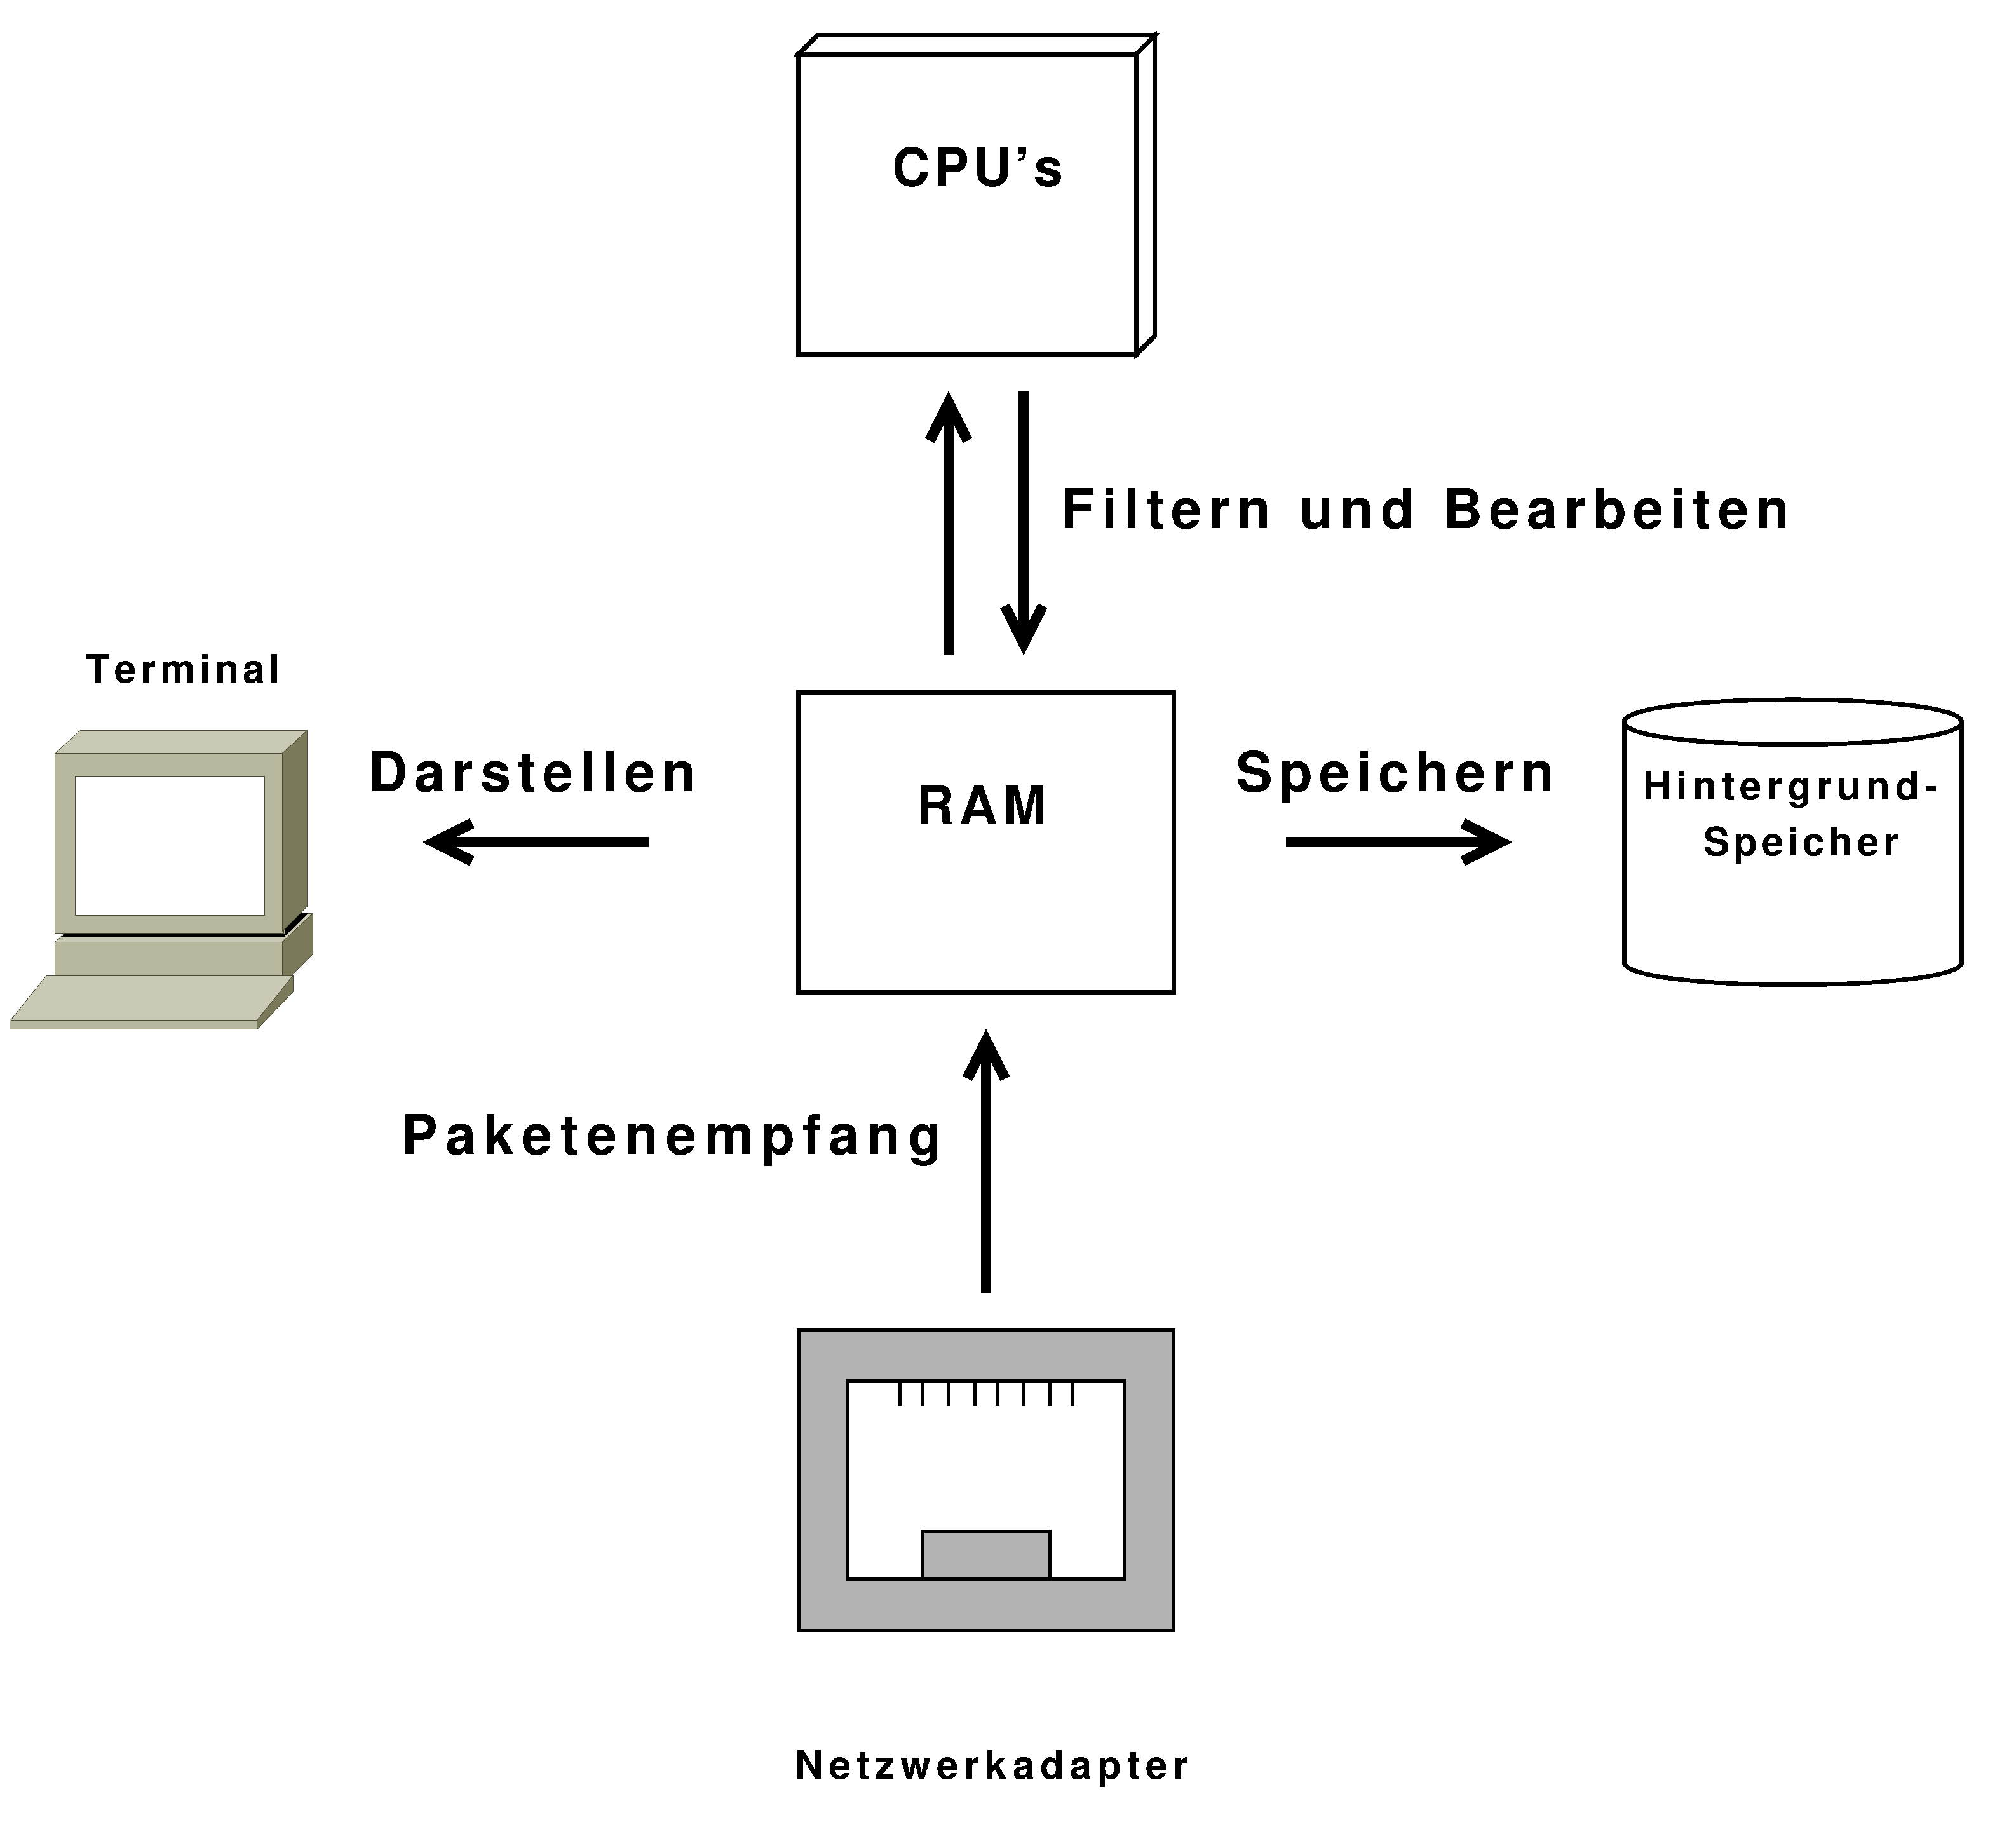
\includegraphics[width=4.0in]{bilder/Capturing}
\caption{Capturing-System}
\label{img:Cap-Sys}
\end{figure}
} 
\subsection{Verwandte Projekte}
\subsubsection*{Zero-Copy BPF Buffers}\label{sec:verw_bpf}
Im Jahr 2007 haben Robert Watson und Christian Peron (Universität Cambridge)
ihre Lösung zur Erhöhung  der Performance von FreeBSD Capturing-Stack
vorgeschlagen und implementiert~\cite{zerocopy}.  Im Rahmen des ``Zero-Copy BPF
Buffers''-Projektes wurde ein neuer Capturing-Stack für das Betriebssystem
FreeBSD entworfen und implementiert.  Im diesem Stack wird das Kopieren der
Paket-Daten in den Userspace, durch Memory-Mapping eliminiert. Dadurch  werden
es keine Kopier-Operationen und keine Systemaufrufe für den Paketzugriff mehr
gebraucht. Da diese Operationen besonders viele CPU Zyklen für ihrer Ausführung
brauchen, verbessert Zero-Copy-Model die Capturing-Performance.\\\\
%
Das Benutzen von Memory-Mapped-Buffers erfordert allerdings ein neues Konzept
für den Zugriff auf Daten from Userspace. Deshalb wurden im Rahmen des
\emph{Zero-Copy} Projektes auch die Libpcap-Funktionen für den Zugriff auf
Pakete im Shared-Buffer angepasst.

%\begin{figure}
%	\begin{center}
%	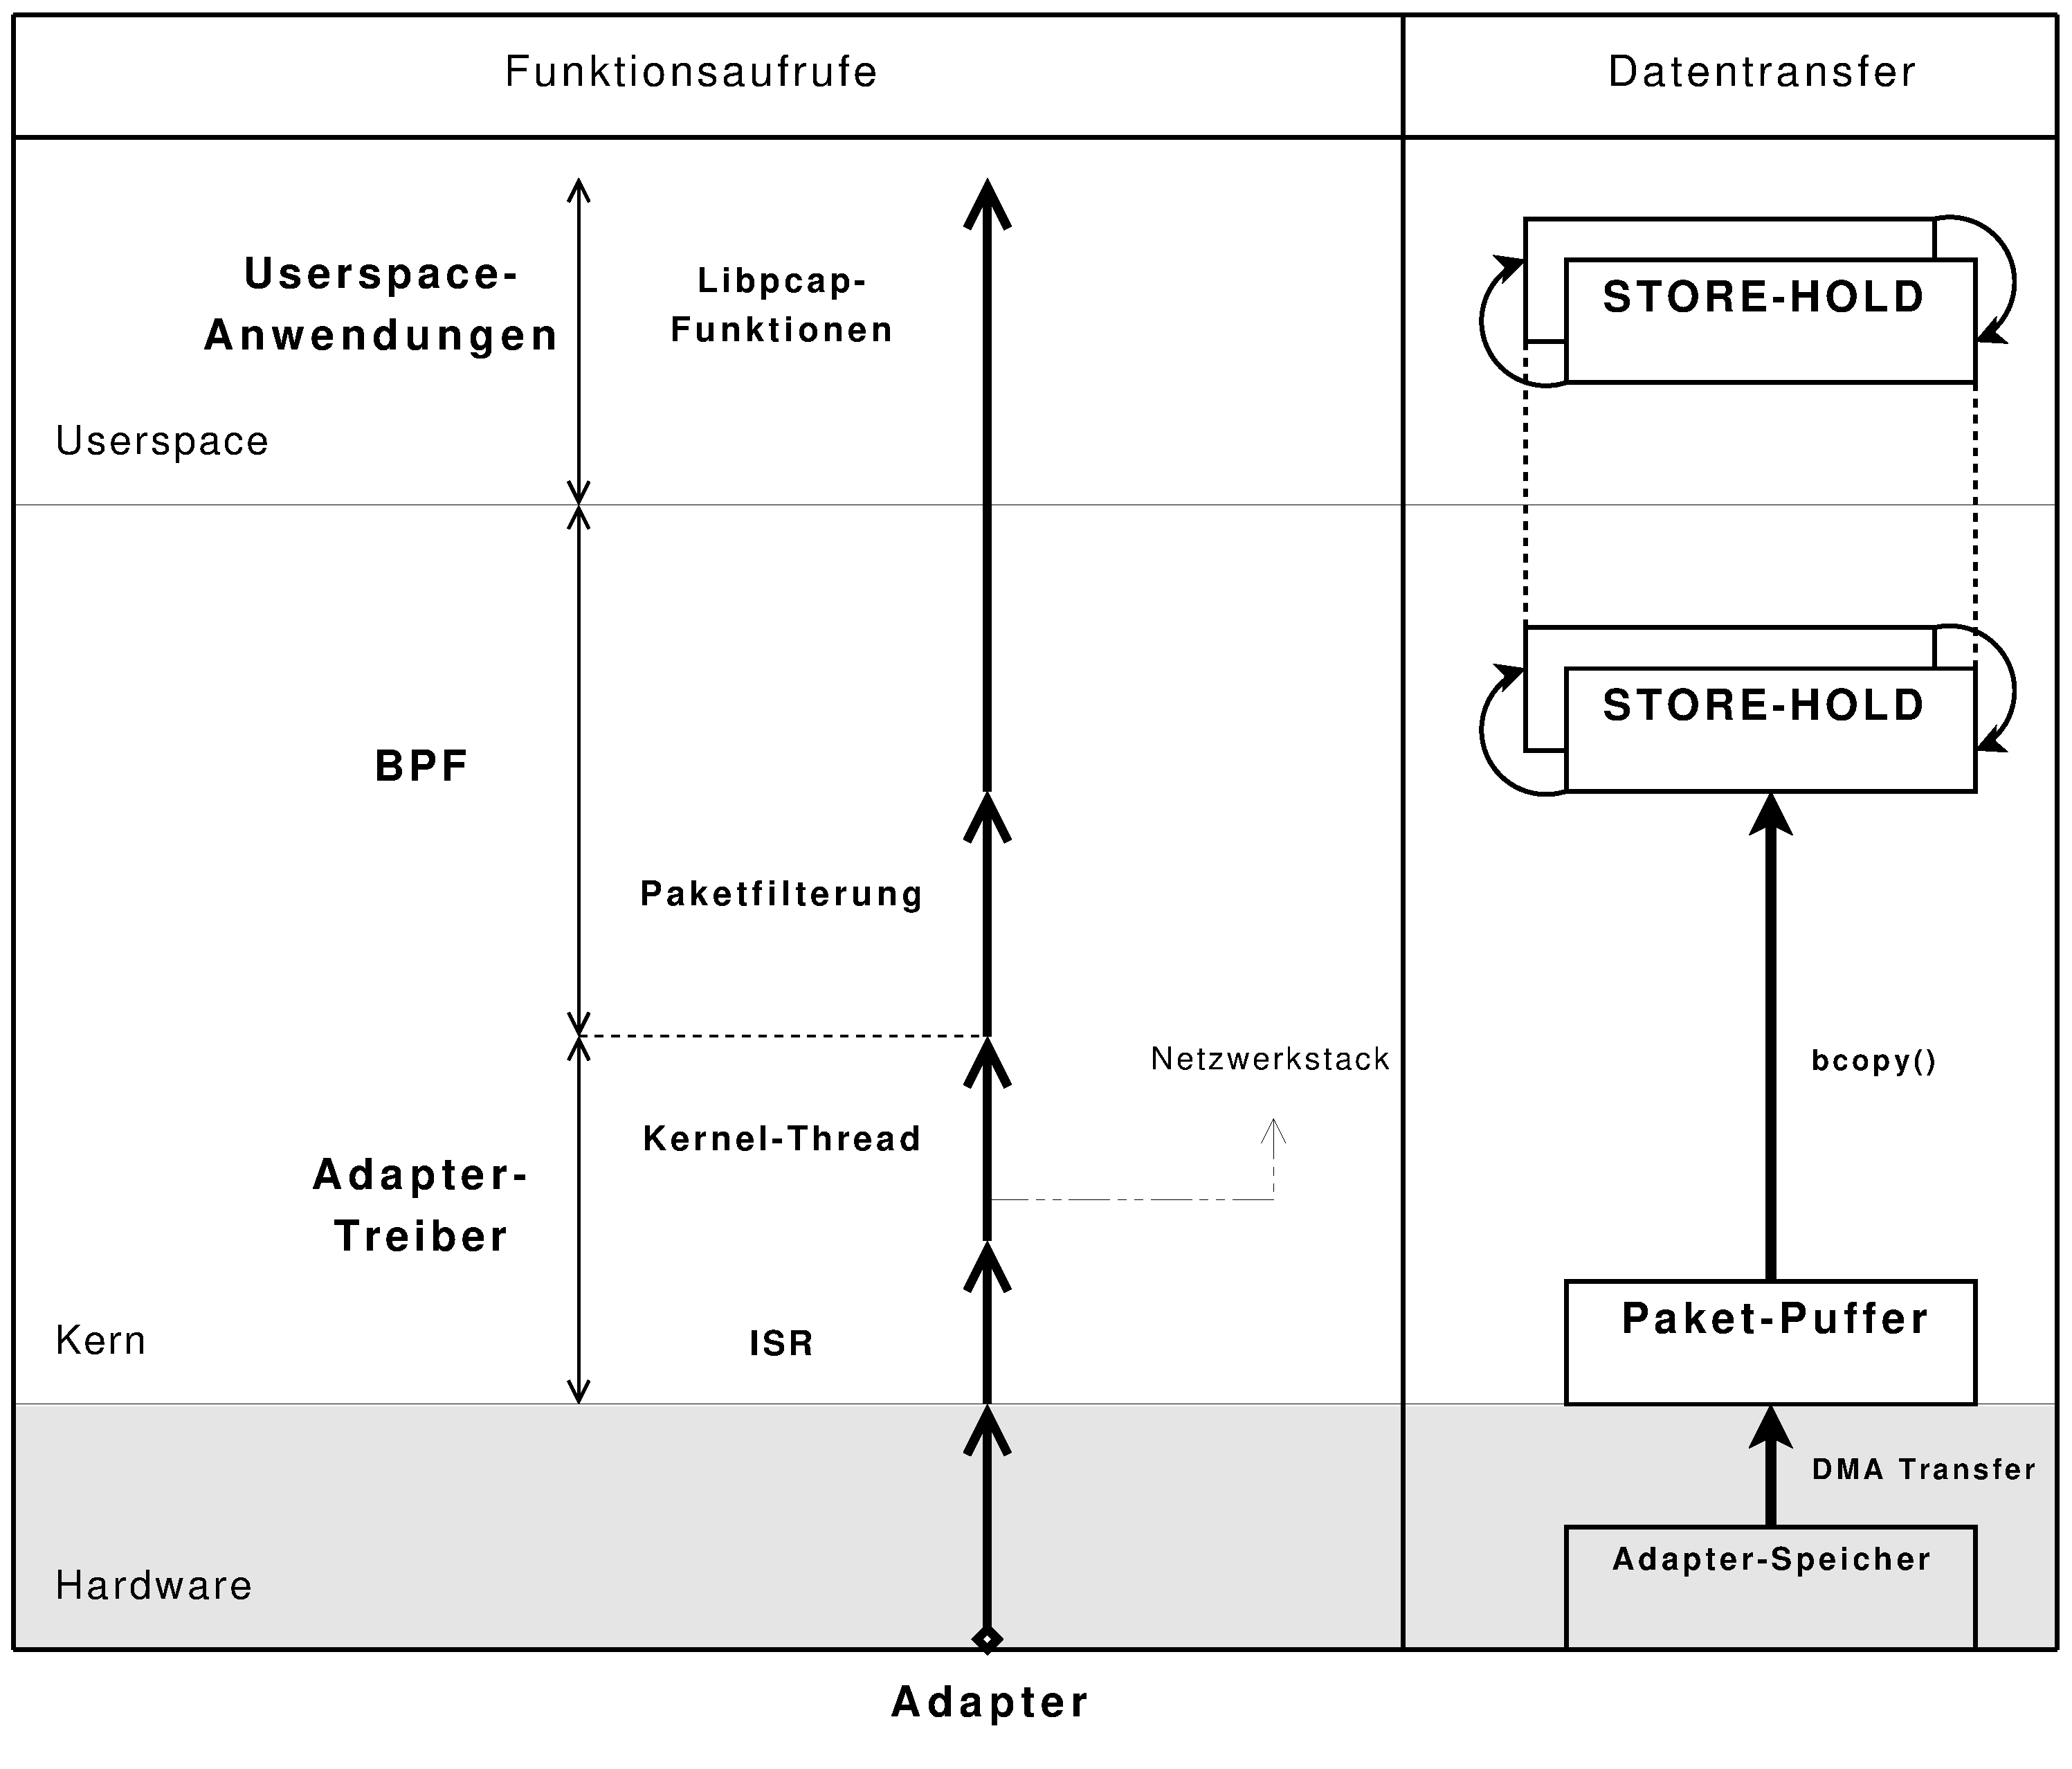
\includegraphics[width=4.9in]{bilder/2copy}
%	\end{center}
%	\caption{Zero-Copy BPF Buffers}
%	\label{img:zc_bpf}
%\end{figure}

\ifthenelse{\boolean{BRIEF}}{}{ 
\subsection{Begriffserklärung}
% \reviewnote{Andi: Warum Definition und Begriffserklärung separat?}

In dieser Diplomarbeit werden oft einige englische Begriffe auftauchen. Sie
haben zwar deutsche Übersetzung, werden aber meistens in ihrer englischen Form
benutzt. Aus diesem Grund gibt es hier eine kurze Begriffserklärung. Auch, weil
der praktische Teil der Diplomarbeit auf einer konkreten Hardware- und
Softwareplattform realisiert wird, sind die Bedeutungen der Begriffe
gezielt dem Kontext der Diplomarbeit angepasst.

\begin{description}
\item[Userspace] ist ein Speicherbereich und Ausführungskontext für
	Useranwendungen.

\item[Kernelspace] ist ein Speicherbereich und Ausführungskontext für den Kern
	des Betriebssystem.

%\reviewnote{Thread is ein Prozess klingt komisch. ggf. Prozess definieren}

\item [Kernel-Thread]
	ist ein Prozess, der vollkommen in Kernelspace ausgeführt wird und keinen 
	direkten Zugriff auf Adressraum eines User-Prozesses hat. Die Kernel-Threads
	werden wie normale Threads in eigenen Threadskontext mit den eigenen Funktions-Stacks
	aber mit einer höhere als bei normalen Threads Prioritäten ausgeführt. 

\item[Interrupt (\emph{Deutsch:} Unterbrechung)] ist ein Ereignis, das den
	Instruktionsfluss auf einer CPU unterbricht und Ausführung einer
	Interrupt-Routine (\emph{Interrupt handler}) auf dieser CPU verursacht.

\item[DMA (\emph{Deutsch:} Speicherdirektzugriff)] bezeichnet eine Art des
	Specherzugriffes, die über Bussystem ohne Beteiligung der CPU realisiert
	ist \cite{dma_wiki}.

\item[Memory-Mapping]  ist eine Funktionalität des Betriebssystem, deren Aufgabe
	es ist, mehrere virtuelle Adressräume auf einen bestimmten physischen
	Speicherraum abzubilden. 

\item[Pointer:] Zeiger

\item[Systemload] ist der prozentuelle Zeitanteil, den CPUs im
	Systemmodus (\emph{protected mode, Ring-0}) verbringen. 

%\reviewnote{Schlecht formuliert:}
\item [Overhead:] Überflüssige Rechenzeiten, Bustransaktionen  und Daten, die
	auf nicht der eigentlichen Aufgabe dienende Prozesse verwendet werden
	müssen.

\item [Descriptor (\emph{Deutsch:} Deskriptor)] ist eine Datenstruktur, die
	zur Beschreibung und Adressierung eines Speichersegmentes dient.
	Descriptor enthält die Anfangsadresse des Segmentes und, eventuell, die
	Länge, die Zugriffsrechte, und andere für das Speichersegment relevante
	Informationen.
\item [Frame] ist Paket auf \emph{link-layer} Ebene. In dieser Diplomarbeit werden
	die Begriffe ``Paket'' und ``Frame'' als Synonyme benutzt. 

\item [NIC (\emph{Network Interfeace Controller})] Netzwerkadapter. In dieser
	Diplomarbeit ist unter diesem Begriff  der Intel Ethernet Gigabit Adapter
	gemeint (siehe \ref{sec:hwsw_voraus}).

\end{description}


\subsection{Struktur der Diplomarbeit}
Das nächste Kapitel \textbf{Grundlagen} präsentiert Hardware- und
Software-Aspekte von Packet-Capturing. Dabei werden zunächst die Funktion der
Hardware vorgestellt, die für die Capturing-Performance relevant ist. Dies
betrifft die Netzwerkkarte, das RAM und den System-Bus.
Unter Software-Aspekten wird der schematisches
Entwurf des Adapter-Treibers und des \emph{Berkley-Packet-Filters} dargestellt.
Außerdem werden in dem Kapitel die Entwurfs-Anforderungen für den neuen
Packet-Capturing-Stack formuliert.\\\\
%
Im Kapitel \textbf{Entwurf} werden Algorithmen zur Verbesserung des FreeBSD
Capturing Stacks vorgestellt. In dem Kapitel werden lediglich logische Lösungen der
Probleme, die bei  Capturing auftauchen, vorgeschlagen. Die Lösung wird zwar
abstrakt dargestellt, basiert dennoch wird auf der konkreten für die Diplomarbeit
vorausgesetzten Hardware.\\\\
%
Im Kapitel \textbf{Implementierung} wird die Struktur der entwickelten Software
vorgestellt. Hierbei werden im Speziellen die Software-Komponenten gezeigt
und kurz erklärt, die für die Umsetzung der im Entwurf vorgestellten
Algorithmen implementiert sind.  \\\\
%
Im Kapitel \textbf{Leistungsbewertung} findet man die Ergebnisse  
des Vergleichs der Performance des FreeBSD-Capturing-Stack im ``generischen''
Fall mit dem neuen, im Rahmen der Diplomarbeit verbesserten, Capturing-Stack. \\\\
%
Im Kapitel \textbf{Schlussfolgerung} wird das wichtigste aus der Diplomarbeit 
in Kurzform dargestellt.  

}

\newpage

\ifthenelse{\boolean{BRIEF}}{
\section{Analyse des standard Paket-Capturing-Stacks in FreeBSD}
}{
\section{Grundlagen}
}
%
In diesem Kapitel werden die für Capturing relevante Aspekte  dargestellt. Es
wird dabei analysiert bei welchen Capturing-Komponenten unter welchen Umständen
Engpässe bei der Paketerfassung auftretten können. Anhand der herausgefundenen
Problemen werden Anforderungen und Ansätze für den Entwurf der neuen
Capturing-Software formuliert.  Zu beachten ist, dass die dargestellten Aspekte
sich vollkomen auf die für die Arbeit vorausgesetzten Hardware und Software
beziehen (siehe Abschnitt \ref{sec:hwsw_voraus}).
%
\ifthenelse{\boolean{BRIEF}}{}{
Obwohl die eigentliche Aufgabe der Diplomarbeit in der Analyse und
Verbesserung der Softwarekomponenten liegt, dennoch ist es unentbehrlich ,
die Funktionsweise der darunterliegenden
Hardwarekomponenten zu kennen.  Dies folgt daraus, dass die Hardware die Rolle
eines Betriebsmittels für die Software-Anwendungen spielt, und deshalb
die Software möglichst effektiv die zur Verfügung
gestellte Hardware-Ressourcen nutzen muss. Dafür muss bekannt werden, wie die
einzelne Hardware-Bestandteile funktionieren.

\subsection{Hardwareaspekte bei Capturing}\label{subsec:hw_cap}
% Bla-bla über dem Inhalt dieses Kapitel
In diesem Abschnitt wird die Funktionsweise der Hardware-Komponenten eines
Capturing-Systems vorgestellt. Dabei werden hauptsächlich die für Performance
des Capturing relevanten Aspekte betrachtet.  Und es wird versucht
herauszufinden, welche der Komponenten den
Capturing-Prozess performancemäßig negativ beeinflussen können, und unter welchen
Umständen dies auftritt.

\subsubsection{Netzwerkadapter}\label{sec:adapter}
In diesem Abschnitt wird beschrieben wie der Adapter die Pakete empfängt und
wie er sie in den RAM weiterleitet. Dieses Wissen ist notwendig für die
Auswertung der Capturing-Performance, weil die Engstellen, die auf diesem
ersten Datenweg vorhanden sind, die höhste theoretische Grenze für Performance des gesamten
Capturing-Prozess auf dem Capturing-System bilden. Außerdem, ist die Kenntnis der
Netzwerkadapter-Funktionen auch für das Implementieren der Capturing-Software
unentbehrlich, denn um die Software für den Zugriff auf ankommende Daten
implementieren zu können, muss man zuerst wissen, auf welche Art und Weise die
Hardware diese Daten zur Verfügung stellt.\\\\
%
Außerdem wird in diesem Kapitel das \emph{Interrupt-Coalescing}-Mechanismus des
Intel Gigabit Adapters erläutert. \emph{Interrupt-Coalescing} erlaubt 
die Interrupt-Rate des Adapters zu steuern und damit die Capturing-Performance  zu 
beeinflussen. \\\\
%
% Sagtest Du schon! -- Andi
%Zu beachten, dass die in diesem Abschnitt betrachteten Hardware-Funktionen sich
%vollkommen auf den für die Diplomarbeit vorausgesetzten \textbf{INTEL Pro
%Ethernet Gigabit Adapter} beziehen (siehe Abschnitt \ref{sec:hwsw_voraus}).

\subsubsection*{Paketempfang und DMA-Transfer in RAM}\label{sec:hw_dma} 
Der Empfang eines Paketes an einem Netzwerkadapter schließt das Erkennen des
Paketes auf dem ``wire'', das Anwenden von Adressfilterung, das Speichern des Paketes
auf dem Adapter-Speicher und dann Transfer des Paketes in den RAM ein.  Im RAM
wird pro Paket ein Paket-Puffer alloziert. Die Größe des Paket-Puffers ist
hardwareabhängig und wird durch das Setzen der entsprechenden Bits in
\emph{Receive Control Register} (\verb+RCTL+) des Adapters
festgelegt~\cite{e1000_sdm}. In dem Fall, wenn der Paket größer als der
Paket-Puffer ist, werden mehrere Paket-Puffer für die Speicherung des Paketes
verwendet.\\\\
% DMA. Deskriptor based DMA.
%\reviewnote{Descriptor oder Deskriptor -- eins von Beiden}
Der Datentransport in den RAM wird per DMA (Direct Memory Access) durchgeführt. Es
gibt unterschiedliche DMA-Arten: die ``klassische'' \emph{Register-Based-DMA}
und die \emph{Deskriptor-Based-DMA}~\cite{dma_desc_base}. Der Intel Gigabit
Adapter verwendet die zweite Variante. Beim Deskriptor-Based-DMA werden alle
für DMA benötigte Daten (Ziel-Adresse, Länge des Speichersegments, etc\ldots)
nicht direkt in den DMA-Registern gespeichert, sondern in einem Array im RAM
abgelegt. Jedes Element des Arrays trägt den Namen ``\emph{Deskriptor}''.
Der Deskriptor enthält die Adresse des Puffers im RAM, an die die Daten beim
DMA-Transfer geschrieben werden und andere Bit-Blöcke, die sowohl für die
Steuerung des DMA-Engine des Adapters, als auch zur Benachrichtigung des
Capturing-Prozesses über den Status der DMA-Operation und über Integrität der
empfangenen Daten dienen(siehe Abbildung \ref{dma-e1000-desc}). Für jeden
Puffer im RAM, an den die Daten vom Gerät transferiert werden, bzw. für jeden
DMA-Transfer, steht genau ein Deskriptor zur Verfügung, wobei jeder
Deskriptor nach Abschluss des Transfers erneut für DMA-Transfers
wiederverwendet werden kann.
\begin{figure} 
\centering 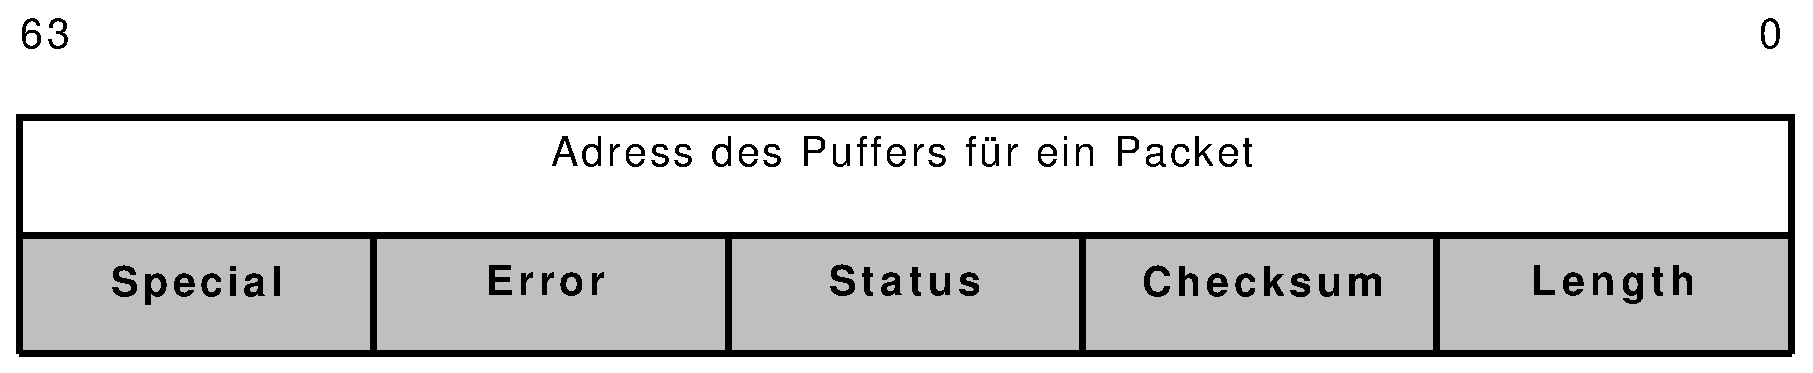
\includegraphics[width=5.0in]{bilder/Decriptor_e1000}
\caption{DMA-Deskriptor von Intel Ethernet Adapters}
\label{dma-e1000-desc}
\end{figure}
% Intel Pro Deskriptor
\subsubsection*{Deskriptor-Format}\label{sec:deskr_format} 
In Abbildung \ref{dma-e1000-desc} ist das Format des Deskriptors des Intel
Gigabit Adapters dargestellt. Die grau unterlegten Bereiche bezeichnen Felder,
die beim Transfer des Paketes in den RAM, von der Hardware verändert werden.
Wenn der Adapter das Paket aus seinem Adapter-Speicher in den Paket-Puffer im
RAM kopiert, setzt er im entsprechenden Deskriptor die Länge (Length) der in
Puffer gespeicherten Daten, die Prüfsumme (Checksum) des ganzen Paketes, den
Status der DMA-Operation und Fehlerinformationen (Errors) \footnote{Siehe
Software Developer’s Manual~\cite{e1000_sdm}, Seiten: 20-24}.\\\\
%
Die Software kann durch das Lesen der vom Adapter in den Deskriptor
geschriebenen Werte den Zustand des DMA-Transfers und die für das empfangene
Paket relevanten Informationen herausfinden. Außerdem kann die Software auch den
neuen Paket-Puffer allozieren und die Adresse des neuen Puffer im gerade
benutzten Deskriptor setzten, sodass beim nächsten Benutzen des Deskriptor, der
DMA-Transfer in den neuen Puffer stattfindet und die Daten im ``alten''
Paket-Puffer nicht überschreibt.
% Deskriptor-Ring-Array
\subsubsection*{Deskriptor-Ringpuffer}\label{sec:deskr_format} 
Der Adapter betreibt Deskriptoren  als einen Ringpuffer (siehe Abbildung
\ref{img:rdrp}). Der Adapter enthält zwei Register: \emph{Receive Descriptor Head
Register} (RDH) und \emph{Receive Descriptor Tail Register} (RDT), welche die
Rolle von \emph{HEAD-} und \emph{TAIL-}Pointers im Ringpuffer spielen und die
Speicherbereiche mit Deskriptoren referenzieren. Jedes mal, wenn der Adapter ein neues Paket
in den RAM schreibt, wird der Wert im RDH-Register inkrementiert, sodass dieser
Wert dem Deskriptor für den nächsten DMA-Transfer entspricht.  Wenn die
Software die Daten aus dem Paket-Puffer gelesen hat, soll sie den Wert im
RDT-Register inkrementieren, aber so, dass dieser Wert dem Deskriptor entspricht,
der den Paket-Puffer mit dem gerade gelesenen Daten referenziert.
Daraus folgt: 
\begin{itemize}
	\item $RDH = RDT \Longleftrightarrow$ Der Ring ist ``voll'':\\ Es gibt
		keine freien Deskriptoren für einen DMA-Transfer. In diesem Fall stoppt
		die Hardware den Datentransfer in den RAM und wartet bis die Software
		die Pakete in den Paket-Puffern liest (bzw. bearbeitet) und den Wert im
		RDT-Register entsprechend erhöht.
	\item $RDT = (RDH - 1)\ mod\ SIZE \Longleftrightarrow$ Der Ring ist
		``leer'':\\ Die Software hat alle Pakete, die vom Adapter in den RAM
		geschrieben wurden,  bearbeitet und wartet jetzt auf das Ankommen von
		neuen Daten bzw. auf das Erhöhen des Wertes im RDH-Register vom
		Adapter.
\end{itemize}
\begin{figure}
\centering 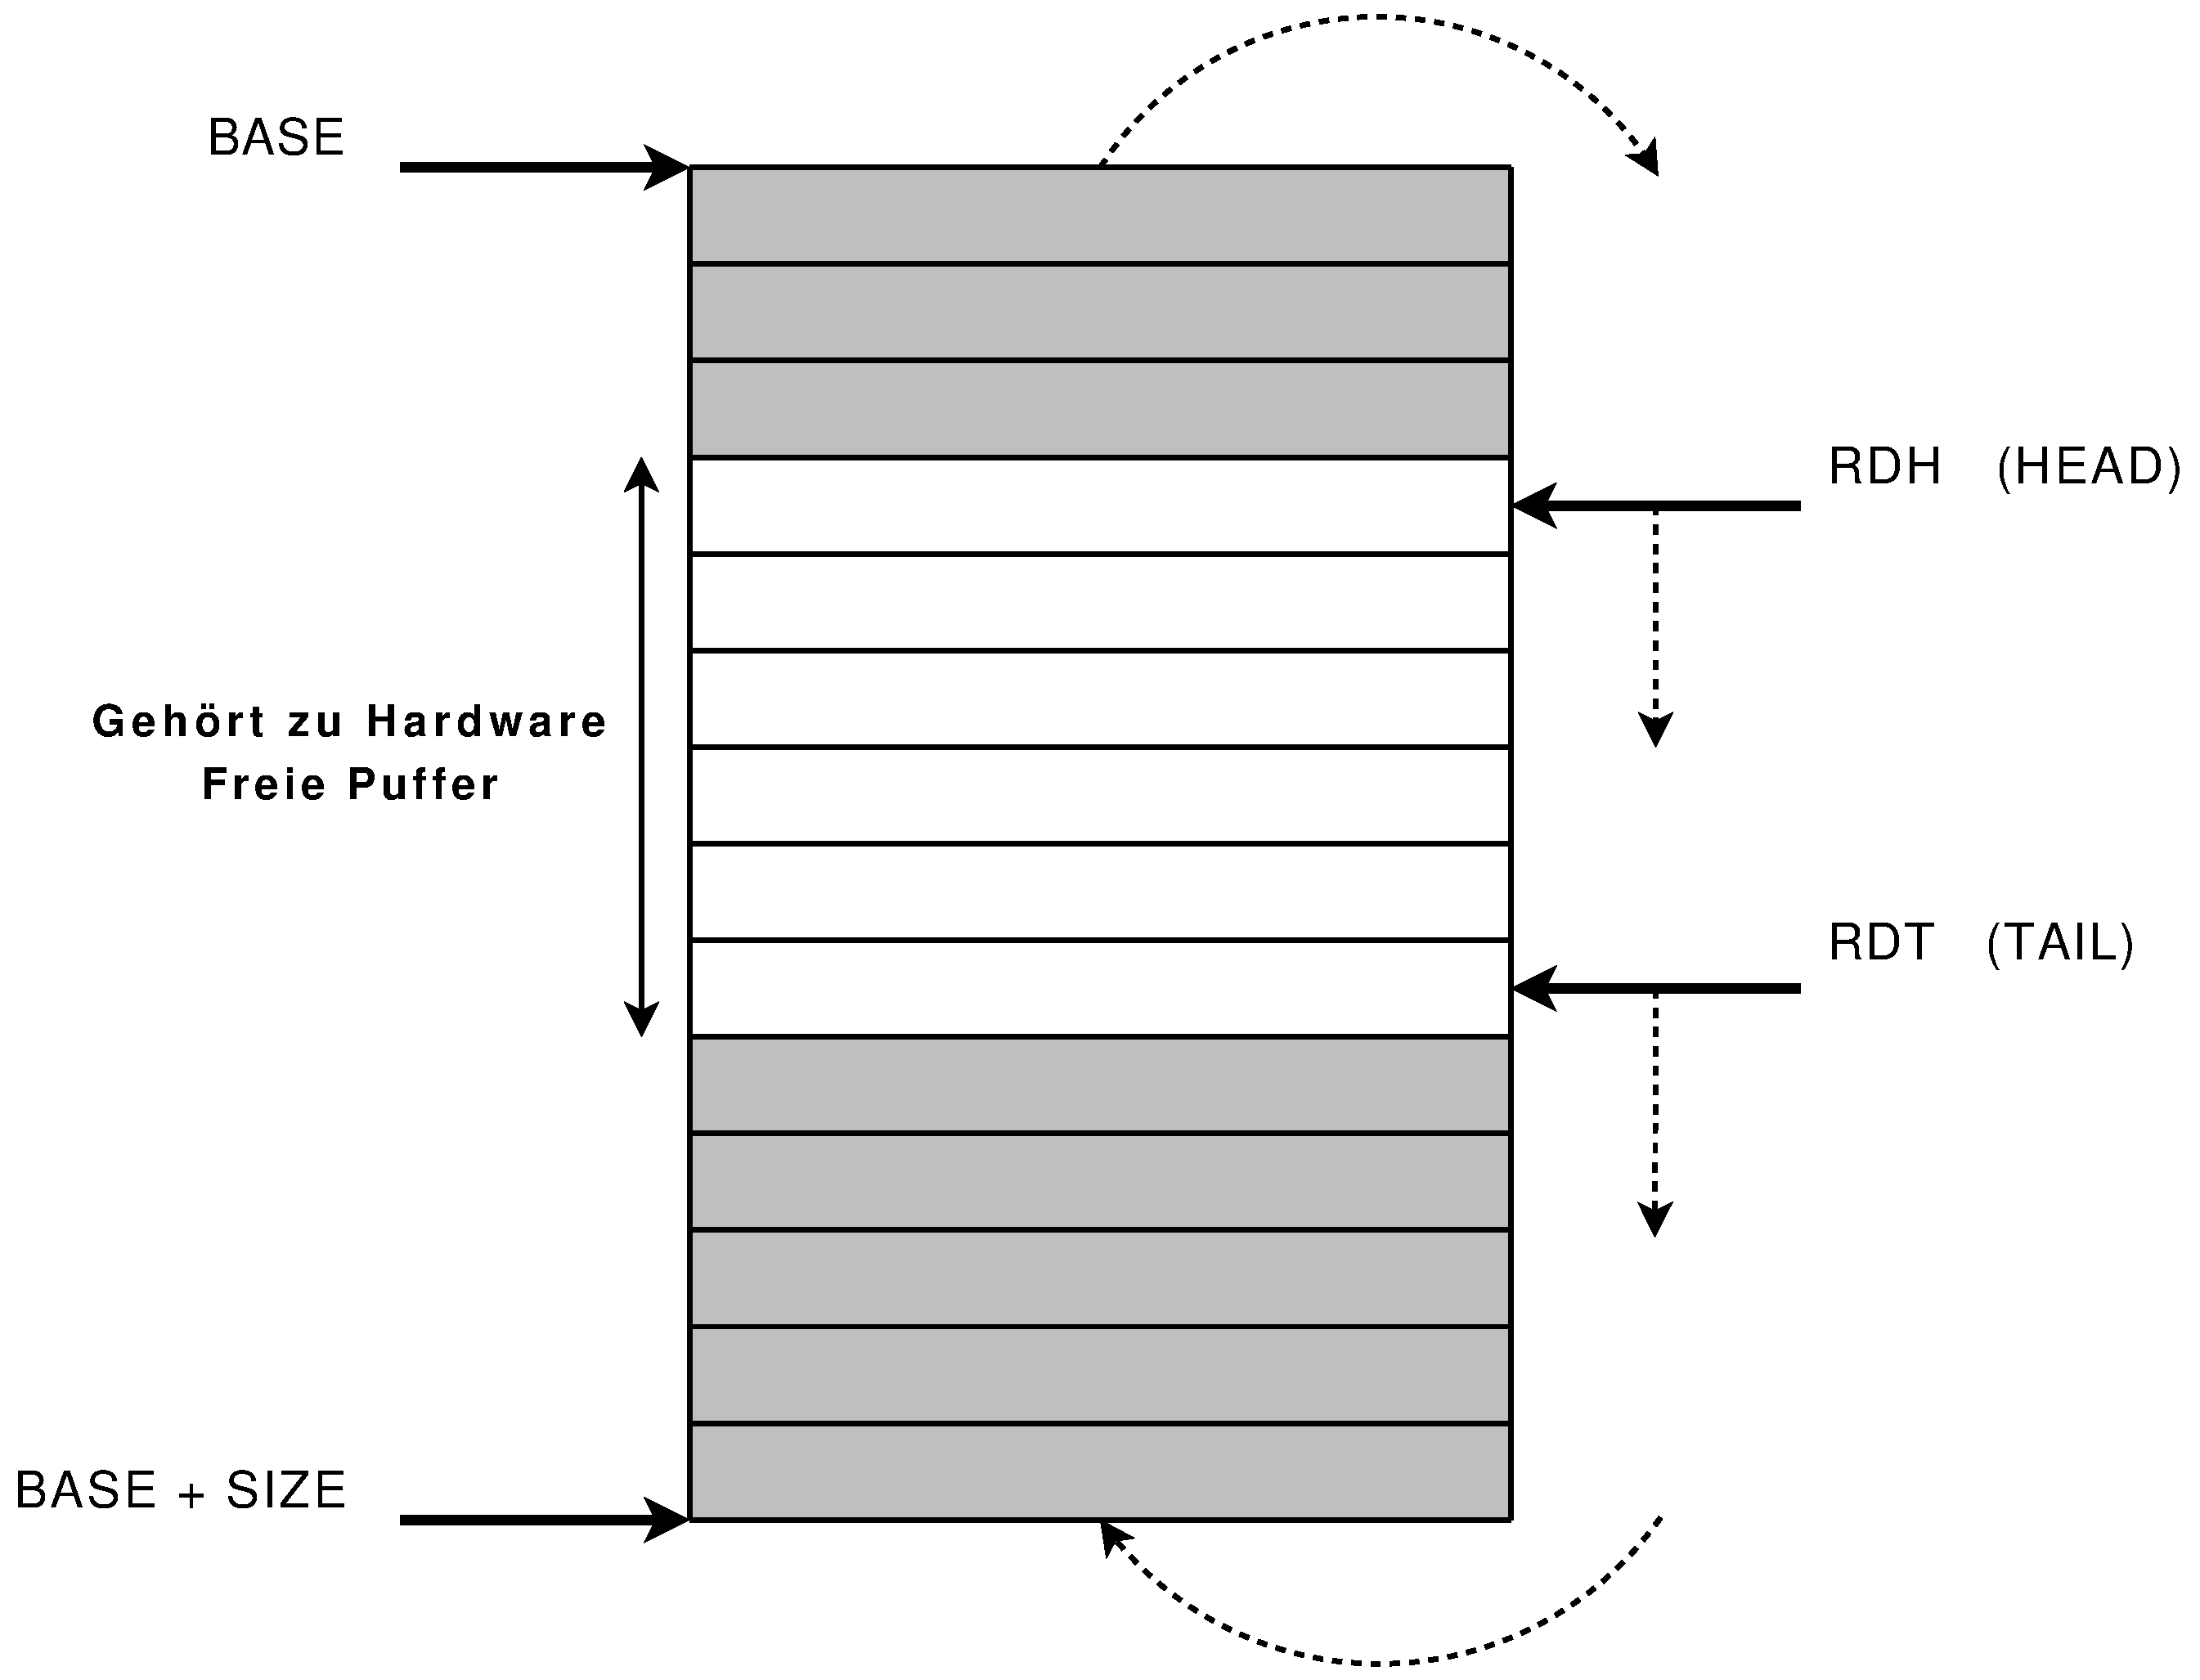
\includegraphics[width=4.0in]{bilder/DescriptorRing}
\caption{Receive Deskriptor Ringpuffer}
\label{img:rdrp}
\end{figure}
% Deskriptor-Array Bild. Beschreibung
In der Abbildung \ref{img:rdrp} ist ein Deskriptor-Ringpuffer dargestellt.  Die
weiss gezeichnete Felder zwischen RDH und RDT, bezeichnen die Deskriptoren, die
für DMA-Transfer der neuen Pakete bereitstehen. Demgegenüber
bezeichnen die graue Felder die Deskriptoren, welche die Paket-Puffer mit den 
neuen Paketen referenzieren, die von der Software noch nicht gelesen wurden.

\subsubsection*{Deskriptor-Fetching}\label{sec:deskr_fetch} 
Um die Werte in den Deskriptoren zu aktualisieren, und um der Software bzw. dem
Adapter die aktualisierten Werte in den Deskriptoren zur Verfügung zu stellen, werden die
Deskriptoren zwischen RAM und Adapter hin- und her kopiert. \\\\
%
Wenn die Software auf den Paket-Puffer mit dem neuen Paket zugegriffen hat,
erhöht sie den Wert im RDT-Register, und stellt damit dem Adapter den
Deskriptor, der den vorher gelesenen Paket-Puffer referenziert, zur Verfügung.
Der Adapter kopiert bei Gelegenheit den Deskriptor in seinen dazu geeigneten
internen Speicher. Und, später, während des  Transfers der aus dem Netz
empfangenen Paketes  in den RAM wird der Deskriptor lokal auf dem Adapter
aktualisiert und wieder zurück in den Deskriptor-Ringpuffer geschrieben.

\subsubsection*{Interrupt}\label{sec:hw_intr}
%\reviewnote{Der letzte Satz hier ist ein fürchterlicher Bandwurmsatz. Mach 3 draus!}
Die Anwesenheit von neuen Paketen im RAM wird vom Adapter durch einen Interrupt
gemeldet.  Die Interrupts, genau gesagt, die Art und Weise, wie die Interrupts
behandelt werden, spielen für die Capturing-Performance eine bedeutende Rolle.
Während der Behandlung eines Adapter-Interrupts sind die Interrupt-Ereignisse
des Adapters gesperrt und das Capturing-System ist nicht mehr in der Lage, das
Ankommen von neuen Paketen zu melden und darauf zu reagieren. Das hat zur
Folge, dass, je länger die Behandlung des Interrupts dauert, die
Wahrscheinlichkeit umso höher ist, dass bevor die Interrupts-Behandlung
abgeschlossen ist, alle freie Paket-Puffer mit neuen Paketen ``gefüllt''
werden. Das führt unvermeidlich zum Verlust der nächsten ankommenden
Pakete.\\\\ 
%
Aus diesem Grund muss die Interrupt-Behandlung-Routine möglichst effizient
implementiert werden und möglichst schnell abgearbeitet werden.
%, um so schnell wie möglich abzuarbeiten, sodass das System
%nicht zu lange im ``Stau'' bleibt und die neue Ereignisse möglichst
%unverzüglich melden und bearbeiten kann, um die Pketverluste zu vermeiden.  
%Die Effizienz der Software 
Die Laufzeit des Interrupt-Handers ist aber noch nicht alles. Wegen des ``Overhead'', den jeder
Interrupt mit sich bringt, spielt auch die Interrupt-Rate eine große Rolle für
Capturing-Performance.\\\\
%
Auf FreeBSD Betriebssystem enthält die Bearbeitung jedes Interrupts 
die folgende Schritte~\cite{freebsd_design}:
%\reviewnote{Was ist ein Hardware-Kontextwechsel??!}
\begin{enumerate}
	\item Hardware und Software Kontextwechsel\footnote{Gemeint ist Umschalten der CPU zwischen Ring-0- und Ring-1-Modus~\cite{pchw} }, die Speicherung von
		CPU-Register, das Wechsel des aktuellen Stack
	\item Zugriff auf die Hardware-Register und Herausfinden der zuständigen
		Interrupt-Service-Routine (ISR)
	\item Aktualisieren der Interrupt-Counters
	\item Ausführen der \emph{Interrupt-Service-Routine}(ISR)
\end{enumerate}
Die Ausführungszeit von ISR (Schritt \textbf{4}) ist variabel und hangt von der
Komplexität der im Interrupt-Kontext ausgeführten Funktionen ab.  Dagegen
bleibt die Ausführungszeit der Schritte \textbf{1} bis \textbf{3}
(eigentlicher Interrupt-Overhead)  konstant und wird bei jeder
Interrupt-Behandlung immer dabei sein.  Die Ausführungszeit der Schritte
\textbf{1} bis \textbf{3} beträgt auf einem konventionellen PC einige
Mikrosekunden~\cite{intrr_coal}, was verursacht, dass bei einer hohe Rate von
Interrupt-Ereignissen (z.B. mehr als $100 000/sec$) ein dominierender Anteil
der CPU-Ressourcen nur für den Interrupt-Overhead verwendet werden kann.
Beim Capturing verursacht das Paket-Verluste.\\\\
%, denn die Anzahl der
%Pakete, die ein Rechnersystem pro ein Zeitintervall empfangen kann, ist
%offensichtlich durch die Anzahl der Pakete, welche die Betriebssystem-Software
%pro diesen Zeitintervall bearbeitet, begrenzt.\\\\
%
Außerdem kann eine hohe Interrupt-Rate das Capturing-System in den
\emph{receive-livelock}-Zustand bringen~\cite{elim_recv_lock}.
\emph{Receive-livelock} ist ein Zustand, in dem das Rechnersystem die ganze
CPU-Zeit lediglich für die Interrupt-Bearbeitung verbraucht und dadurch keine
CPU-Ressourcen für die Ausführung anderer Capturing-Prozesse freigibt. Falls die
Rate der ankommenden Pakete so hoch ist, dass die dadurch enstehende
Interrupt-Load die anderen Prozesse stark vernachlässigt, können 
Paketverluste enstehen, denn die Capturing-Software wird unter FreeBSD sowohl im
Interrupt-Kontext als auch im Userspace ausgeführt.

\subsubsection*{Interrupt-Coalescing}\label{sec:intr_coal}
Zur Beseitigung des receive-livelock-Problems und Minimierung des gesamten
Interrupts-Overhead gibt es die unterschiedliche
Lösungsansätze~\cite{elim_recv_lock, intrr_mod}. Eine davon,
\emph{Interrupt-Coalescing}, wird auf dem Intel Gigabit Adapter verwendet.
Unter dem Begriff Interrupt-Coalescing versteht man das Zusammenfassen von
Interrupts von mehreren Ereignissen zu einem einzigen Interrupts.
%versteckt sich ein Interrupt-Mechanismus
%bei dem jedes Interrupt zur Bearbeitung mehrerer Ereignisse erzeugt werden
%kann. 
In unserem Fall bedeutet dies, dass im Lauf einer Interrupts-Behandlung
nicht nur ein, sondern mehrere empfangene Pakete zusammen bearbeitet werden
können.  Damit lässt sich die Interrupt-Rate reduzieren, was auch zur
Minimierung den gesamten Interrupt-Overhead und gleichzeitig zur Vergrößerung
des Datendurchsatzes bei Capturing führt.\\\\
%
Interrupt-Coalescing wird auf dem Adapter mit Hilfe von drei Timern realisiert~\cite{intrr_mod}:
\begin{description}
	\item[Absolute-Delay-Timer:] Verzögert das Interrupt-Ereignis um ein
		bestimmtes Zeit-Interval (siehe Abbildung \ref{rat}). Der Timer wird nach
		dem Transfer des ersten Paketes in den RAM initialisiert und
		gestartet. Der Timer wird generiert nach dem Ablauf des im
		\verb+RADV+-Register~\cite{e1000_sdm} gesetzten Interval einen Interrupt.
		Nach dem Interrupt, sobald das neue Paket in den RAM
		transferiert wird, wird der Absolute-Timer wieder reinitialisiert und
		gestartet. Der Wert im \verb+RADV+-Register kann durch den
		\emph{sysctl}-Befehl~\cite{man_sysctl} gesetzt werden:
		\begin{equation}
			\verb+# sysctl dev.em.0.rx_abs_int_delay N+
		\end{equation}
%
	\item[Packet-Delay-Timer:] Wie auch der Absolute-Delay-Timer verzögert auch dieser Time
	        nach dem Empfang eines Paketes das Interrupt-Ereignis um ein bestimmtes
		Zeit-Interval (siehe Abbildung \ref{rpt}).  Der Packet-Timer wird aber
		nach jedem Transfer eines neuen Paketes in den RAM jedes mal
		reinitialisiert und wieder gestartet. Der Interrupt des Timers findet
		daher nach Ablauf des Zeit-Intervals nur
		dann statt, wenn während des Zeitintervalls keine neue Pakete vom
		Adapter in den RAM übertragen werden. Das Zeit-Intervall für
		Packet-Timer wird im
		\verb+RDTR+-Register~\cite{e1000_sdm} gesetzt:
		\begin{equation}
			\verb+# sysctl dev.em.0.rx_int_delay N+
		\end{equation}
%
	\item[Interrupt-Throttle-Timer:] Bestimmt eine minimale
		inter-Interrupt-delay für den Adapter. Damit wird  gleichzeitig für
		\emph{receive} und \emph{transmit} eine maximale Interrupt-Rate
		garantiert. Der minimale Zeit-Interval zwischen zwei Interrupts wird in
		\verb+ITR+-Register~\cite{e1000_sdm} gesetzt.\\\\
		%
		Für das Setzen des Wertes in den \verb+ITR+-Register ist kein
		\emph{sysctl} vorgesehen. Um \verb+ITR+ zu setzen, muss man in den Code
		des Treibers über die folgende Makrodefinition die maximale Anzahl der
		Interrupts pro eine Sekunde eingeben: 
		\begin{equation}
			\verb+#define MAX_INTS_PER_SEC        8000+
		\end{equation}
\end{description}
\begin{figure}
\centering 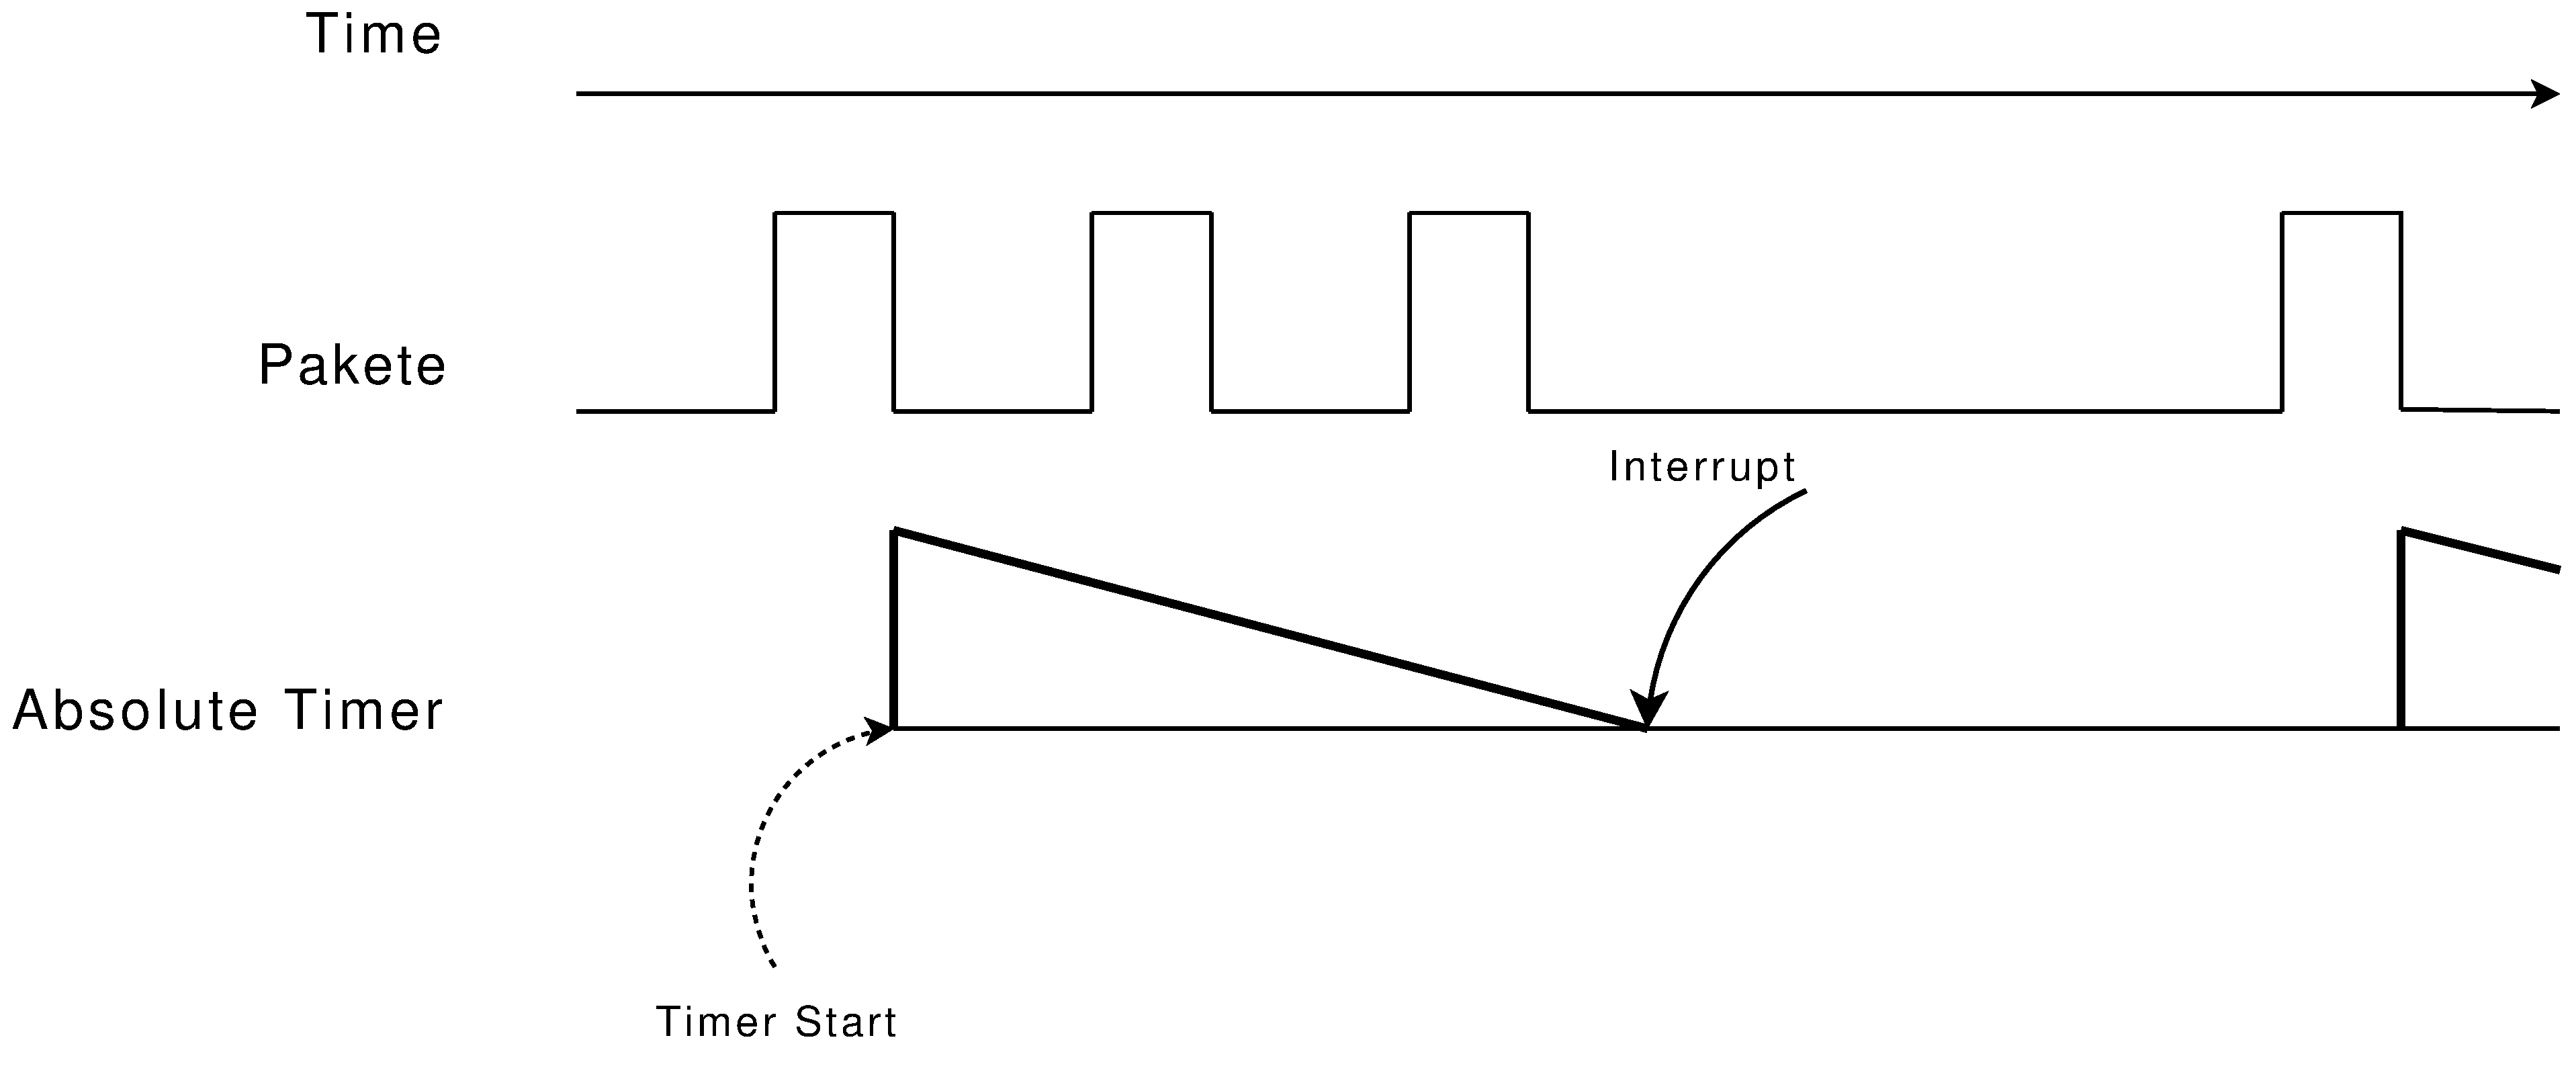
\includegraphics[width=4.0in]{bilder/AbsoluteTimer}
\caption{Absolute Delay Timer}
\label{rat}
\end{figure}
%
\begin{figure}
\centering 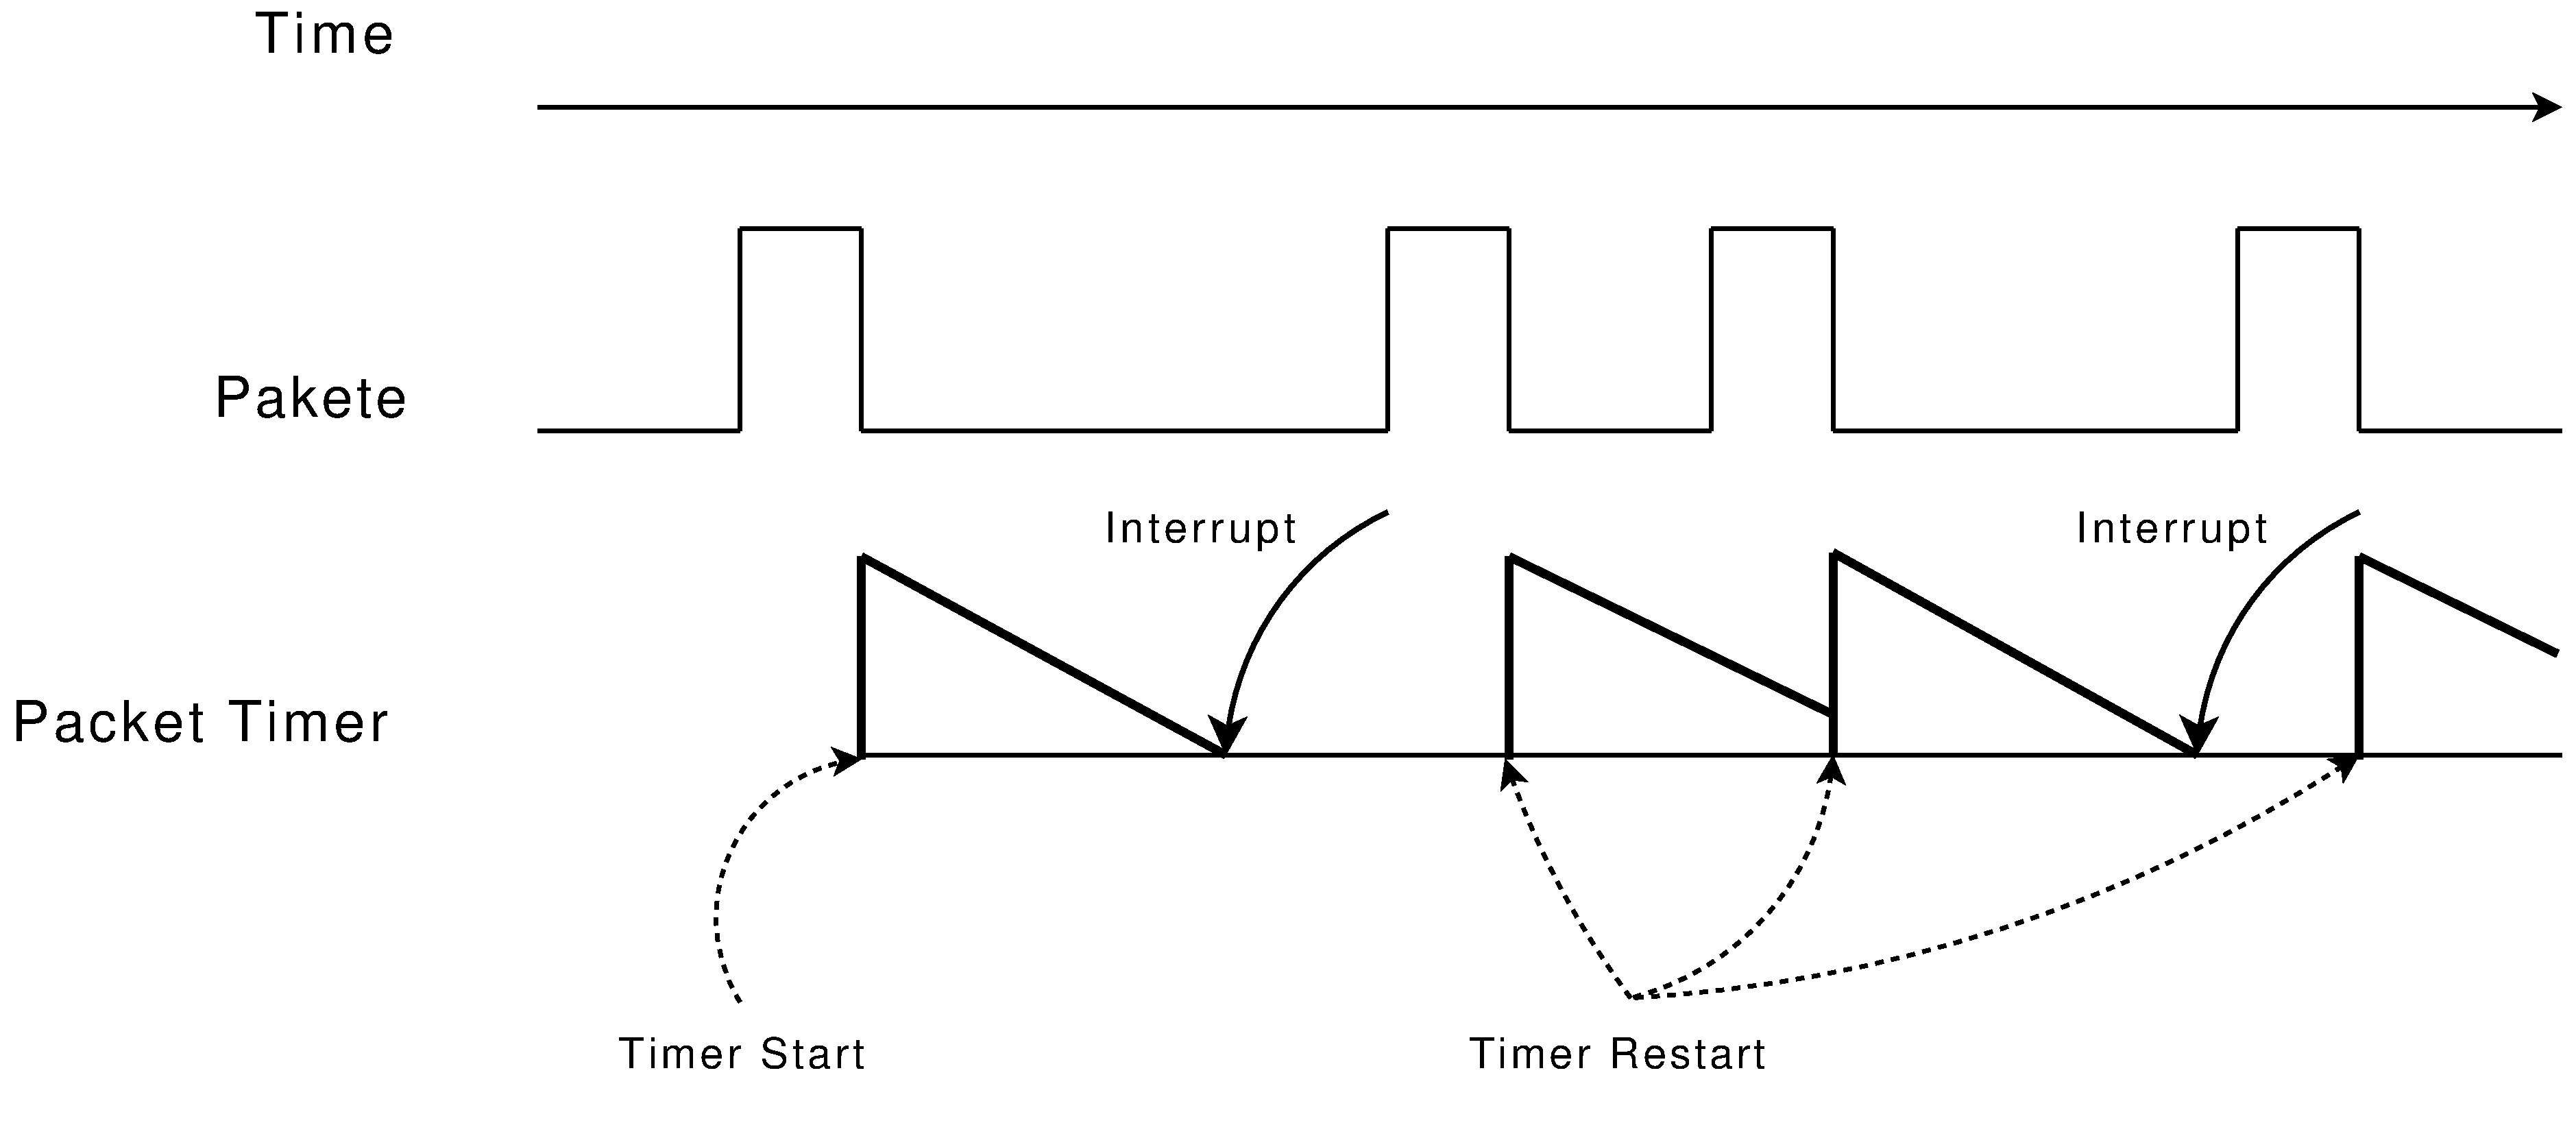
\includegraphics[width=4.0in]{bilder/PacketTimer}
\caption{Packet Delay Timer}
\label{rpt}
\end{figure}
%
Die obengenannten Timer minimieren die Interrupt-Rate durch Verzögerung der
Interrupt-Ereignisse. Bei einer hohen ständigen Paket-Rate ist der
Absolute-Timer die primäre Interrupt-Quelle. Dagegen ist der Packet-Timer die
Ursache der meisten Interrupts, wenn die Paket-Rate klein ist, oder, wenn der
Verkehr  kurze \emph{Bursts} enthält. Die beiden Timer können aber nicht immer
die eine vorhersagbare Interrupt-Rate garantieren.  Erstens git es
für das Senden von Daten ein identisches Paar von Timern für die
für die Transmit-Interrupts. Diese zwei
Timer-Paare arbeiten unabhängig voneinander und können
infolgedessen gegenseitig Ihr Verhalten stören. Zweitens ist der Verkehr in
Netzen meistens unvorhersagbar. Dies kann beim Benutzen von Absolute- und
Packet-Timers eine nicht ständige oder sogar explosive Interrupt-Rate
verursachen.
Dieser Effekt wird durch Benutzung von Interrupt-Throttling beseitigt.
Interrupt-Throttling funktioniert unabhängig von allen anderen
Interrupt-Quellen und wird nicht durch die Verkehrsrate
beeinflusst~\cite{intrr_mod}.
%
\subsubsection*{Adapter: Einfluss auf Capturing}\label{sec:adapt_perf_analyse}
Die Aufgabe des Netzwerk-Adapters beim Capturing ist es, die Pakete aus dem
Netz zu empfangen, sie in den RAM zu schreiben und durch das Interrupt dem
Rechnersystem Bescheid über die neue Pakete im RAM zu geben.\\\\
Der Durchsatz beim Datentransfer vom Adapter in den RAM ist zum großen Teil 
durch Performance-Eigenschaften des Bussystems beeinflusst. Der Adapter selbst 
kann auf unterschiedlicher Art und Weise die zur Verfügung stehende 
Bussystem nutzen. Dieses Vorgehen ist aber auf dem Adapter ``hardgecodet'' und kann 
nicht optimiert werden.\\\\
Anders sieht es mit mit den Interrupts aus. Die Interrupt-Rate kann durch
\emph{sysctl}-Variablen auf dem Adapter beliebig geändert werden.
\emph{Interrupt-Coalescing}-Mechanism erlaubt durch das Verzögerung der
Interrupt-Ereignisses den gesamten Interrupt-Overhead zu minimieren un dadurch
den Datendurchsatz bei Capturing zu erhöhen.\\\\
%
Zu beachten aber, dass zu große Verzögerung des Interrupt-Ereignisses auf dem Adapter
auch einige Nachteile bringen kann:
\begin{itemize}
	\item Da mehrere Pakete in einem Interrupt bearbeitet werden,
		kann die Interruptverzögerung Zeitliche Paket-Verhältnisse
		verfälschen, was weniger korrekte Paket-Zeitstempeln und 
		dadurch die ungenaue Verkehrsanalyse verursachen kann.

	\item Bei einer hohen Verkehrsrate können zu große inter-Interrupt-delays,
		auch Paketverluste verursachen.  % \reviewnote{Wie??}
\end{itemize}
Aus den obengenannten Gründen folgt, dass die Interrupt-Rate sowohl nicht zu
groß als auch nicht zu klein gesetzt werden muss, um die Paketverluste und
Timing-Verfälschungen zu vermeiden.\\\\
%
Per default im aktuellen FreeBSD-7.x für Interrupts-Verzögerung wird lediglich
\emph{Interrupt-Throttling} benutzt. Per Default wird \emph{Throttling} so
gesetzt, dass der Adapter maximal 8000 Interrupts pro Sekunde generieren kann.
Das Benutzen der Paket- und Absolut-Timern wird im aktuellen FreeBSD von den
Treiber-Entwickler nicht empfohlen~\cite{man_em}. 
%
\subsubsection{Bussystem: PCI, PCI-X, PCIe}\label{sec:grund_bussyst}
Das PCI-Bus verbindet den Netzwerkadapter mit dem RAM. Daraus folgt, dass der
Datendurchsatz beim Datentransfer vom Adapter in den RAM von der maximalen
Leistungsfähigkeit des Busses begrenzt wird.\\\\
%
Es gibt unterschiedliche PCI-Varianten: PCI, PCI-X, PCIe. Die theoretischen
Datentransferraten  der klassischen PCI und PCI-X scheinen auf dem ersten Blick
für den Netzverkehr 1Gbit/sec ausreichend zu sein~\cite{lodb_wiki}.
Das ist aber leider nicht immer der Fall. Die Datenübertragung an den
beiden Bussystemen hat bei jedem Datentransfer einen bestimmten Overhead, der
aus den folgenden Faktoren entsteht~\cite{pchw}: 
\begin{itemize}
	\item Handshaking: 
		\begin{itemize}
			\item Für die Verbindungsaufbau werden einige Bus-Transaktionen
				benötigt.
		\end{itemize}

	\item Zeitmultiplexing: 
		\begin{itemize} 
			\item Der Bus kann nicht gleichzeitig für mehrere parallele
				Datentransfers benutzt werden. Außerdem stehen die Busleitungen
				sowohl für die Daten als auch für die Adressen zur Verfügung
				und können bei einer Bus-Transaktion entweder für Datentransfer
				oder für Adressentransfer benutzt werden.
		\end{itemize}
	\item Arbitrierung: 
		\begin{itemize} 
			\item Da der Bus nicht gleichzeitig von mehreren
				Hardware-Komponenten benutzt werden kann, werden einige
				Bus-Transaktionen für Arbitrierung gebraucht. 
		\end{itemize} 
\end{itemize}
Das hat zur Folge, dass die effektive Datentransferrate eines Busses umso niedriger ist,
je mehr Bus-Transaktionen für die Übertragung der Datenmenge benötigt werden.
Der PCI-Bus kann aber eine Datenmenge, die kontinuierlich in den RAM geschrieben werden soll, im 
Burst-Modus, ohne zusätzliche  Adressübertragung für jeden Datenwort-Transfer,
erledigen. Dies kann beim Transfer grosser Datenmengen die Anzahl der benötigen
Bus-Transaktionen und damit den Overhead wesentlich verringern.\\\\
%
PCIe ist mit dem Unterschied zu dem konventionellen PCI kein \emph{shared}
Bussystem, sondern eine separate serielle Punkt-zu-Punkt-Verbindung. Einzelne
Komponenten werden über Switches verbunden. Das ermöglicht die direkte
Verbindungen zwischen einzelnen Geräten herzustellen, so dass die
Kommunikation einzelner Geräte untereinander die erreichbare Datenrate anderer
Geräte nicht beeinflusst.

\subsubsection*{Bussystem: Einfluss auf Capturing}\label{sec:bus_einfl_auf_cap}
Die minimale Datentransfer-Einheit für den Intel Gigabit Adapter ist ein
Paket-Puffer. Jede
Datenübertragung in den Paket-Puffer benötigt eine Reinitialisierung des
DMA-Engine des Adapters und den Aufbau des Transfers über PCI-Bus.  Wenn wir davon
ausgehen, dass die Paket-Größe kleiner als die Paket-Puffer-Größe ist, und dadurch
pro Paket genau einen Paket-Puffer verwendet wird, skaliert der
Bus-Transaktion-Overhead beim Datentransfer hauptsächlich mit der Paketanzahl,
nicht mit der übertragenen Datenmenge.\\\\
%
Wenn die ``gecapturte`` Datenmenge hauptsächlich aus den kleinen Paketen
entsteht, dann verursacht sie einen größeren Overhead bei ihrem Transfer über
den Bus in den RAM als die gleiche Datenmenge, die aber aus den größeren
Paketen entstehen würde. Das hat zur Folge, dass der Datenweg über den PCI-Bus
umso enger wird, je kleiner die Pakete beim Capturing sind.
 
\subsubsection{RAM}\label{sec:ram}
Erst nach dem Transfer in den RAM stehen die erfassten Pakete für
die Software-Anwendungen zur Verfügung. Die Software greift auf die Daten im RAM
zu, filtert bzw. bearbeitet sie und danach ggf. trifft die Entscheidung über
Darstellung der Informationen aus den Paketen oder Speicherung  diesen auf der
Festplatte.\\\\
%
Die Geschwindigkeit, mit der die im RAM befindlichen Daten bearbeitet werden
können, ist von der Leistung des RAM-Speichers und des Prozessorbusses abhängig, weil
die CPU für die Ausführung der Operationen auf Daten, erstmal diese Daten aus
dem Speicher holen muss.\\\\
%
Die effektive Datentransferrate bei der Datenübertragung zwischen den RAM und CPU
kann sich von den theoretischen Werten sehr stark unterscheiden. 
Es gibt einige Benchmarks wie \emph{Stream}~\cite{web_stream} und
\emph{lmbench}~\cite{web_lmbench}, die es erlauben, die effektive 
Datentransferrate zwischen CPU und RAM zu messen.

\subsubsection*{RAM: Einfluss auf Capturing}\label{sec:ram_einfl_auf_cap}
Zu beachten ist, dass die mit Hilfe der Benchmarks gemessene effektive
Speicherbandbreite nicht der einzige Faktor für Performance der Bearbeitung der
im RAM befindlichen Pakete ist. Der Software-Prozess kann während
Paketbearbeitung für jedes Paket mehrere Kopie-Operationen durchführen, was die
Menge der durch den Prozessor-Bus transferierenden Daten vergrößern und damit
diesen Datenweg zur einer Engstelle machen kann.\\\\
%
In unserem Fall bedeutet das, dass um herauszufinden, ob der RAM beim Capturing
eine Engstelle ist, muss man genau den Capturing-Algorithmus kennen, und zwar 
wieviele Kopie-Operationen pro Paket gemacht werden. 
\subsubsection{CPU}\label{sec:cpu}
Die CPU-Leistung ist in den letzten Jahrzehnten wesentlich stärker
gewachsen als die der anderen Hardwarekomponenten eines Computers. 
Damit ist es eher unwahrscheinlich, dass die CPU die
Engstelle beim Capturing darstellt, außer, wenn die 
Software-Anwendung sie sehr ineffizient
benutzt (z.B. durch Ausführen mehrerer unnötigen Operationen).\\\\
%
Dennoch gibt es einige Kriterien an den modernen CPU-Architekturen, welche die
Performance eines Rechen-Prozesses negativ beeinflussen können. Es handelt sich
vor allem um die Multi-Core-Prozessoren. Sie können simultan mehrere Prozesse
gleichzeitig ausführen, was einen Performance-Zuwachs ermöglicht. Auch
wegen der Problemen mit der Datenlokalität, können die Multi-Core-Systeme die
Ausführungszeiten von einigen Datenbearbeitungsfunktionen verlängern.\\\\
%
Die Lösung dafür ist \emph{Prozessoraffinität}. Unter diesem Begriff versteckt
sich ein Mechanismus, mit dem das Betriebssystem für jeden Thread im System einen 
bestimmten CPU-Core für seine Ausführung zuweisen kann. Damit lassen es sich 
Prozesse, die auf gleiche Daten im RAM zugreifen, möglichst auf dem gleichen 
CPU-Core auszuführen.
%
\subsubsection*{CPU: Einfluss auf  Capturing}\label{sec:cpu_einfl_auf_cap}
Weil das Capturing mit Hilfe von mehreren Prozessen (ISR, BPF,
Libpcap-Anwendungen, etc\ldots) ausgeführt wird und auch gemeinsam
benutzte Datenstrukturen beansprucht, soll die Verteilung von diesen Prozessen
auf unterschiedlichen CPU's so sein, dass die Zeit für die
Interprozesskommunikation die gesamte Performance mit wachsender Anzahl 
von Prozessoren nicht verschlechtert.\\\\
%
Im aktuellen FreeBSD-7.2 ist einen neuen Scheduler \emph{ULE}~\cite{bsd_ule} per
Default gesetzt, der zusammen mit dem Programm \emph{cpuset}~\cite{man_cpuset}
vielfältige Funktionen zum Einstellen der Prozessoraffinität zur Verfügung stellt und
erlaubt, für die Threads-Gruppen eine bestimmte CPU zu zuweisen.

}
\subsection{Softwareaspekte bei Capturing}\label{subsec:sw_cap}
In FreeBSD besteht der Capturing-Stack aus mehreren Komponenten.  Das sind der
Netzwerk-Treiber, die Software für die Paketfilterung und die
User-Anwendungen, die ggf.  Libpcap-Funktionen für den Zugriff auf empfangene
Pakete benutzen (siehe Abbildung \ref{bsd_cap_stack}).\\\\
%
Beim Capturing wird jedes aus dem Netz empfangene Paket zuerst in den internen
Speicher des Netzwerk-Adapters kopiert. Sobald es möglich ist, macht der
Adapter den DMA-Transfer der vorhandenen Pakete in den RAM und meldet dies
durch ein Interrupt. Weiter werden die Paket-Daten von der Paketfilter-Software
(BPF\footnote{Berkley Packet Filter}) bearbeitet. Nach der Bearbeitung bzw.
Filterung werden die Pakete von einer Userspace-Anwendung geholt,
weiterbearbeitet und eventuell auf der Festplatte gespeichert oder ggf. auf dem
Terminal dargestellt.\\\\
%
Die Funktionen des FreeBSD-Packet-Capturing-Stacks sind in mehreren
Papers~\cite{bpf_paper, fabian_da} und Manuals~\cite{man_bpf} ausführlich
beschrieben.  Deshalb enthält der weitere Text nur eine einführende
Beschreibung des Themas.  Eingehend werden lediglich die Aspekte betrachtet,
die für Analyse und Verbesserung der Performance des aktuellen Capturing-Stack
relevant sind.
\begin{figure}
\centering 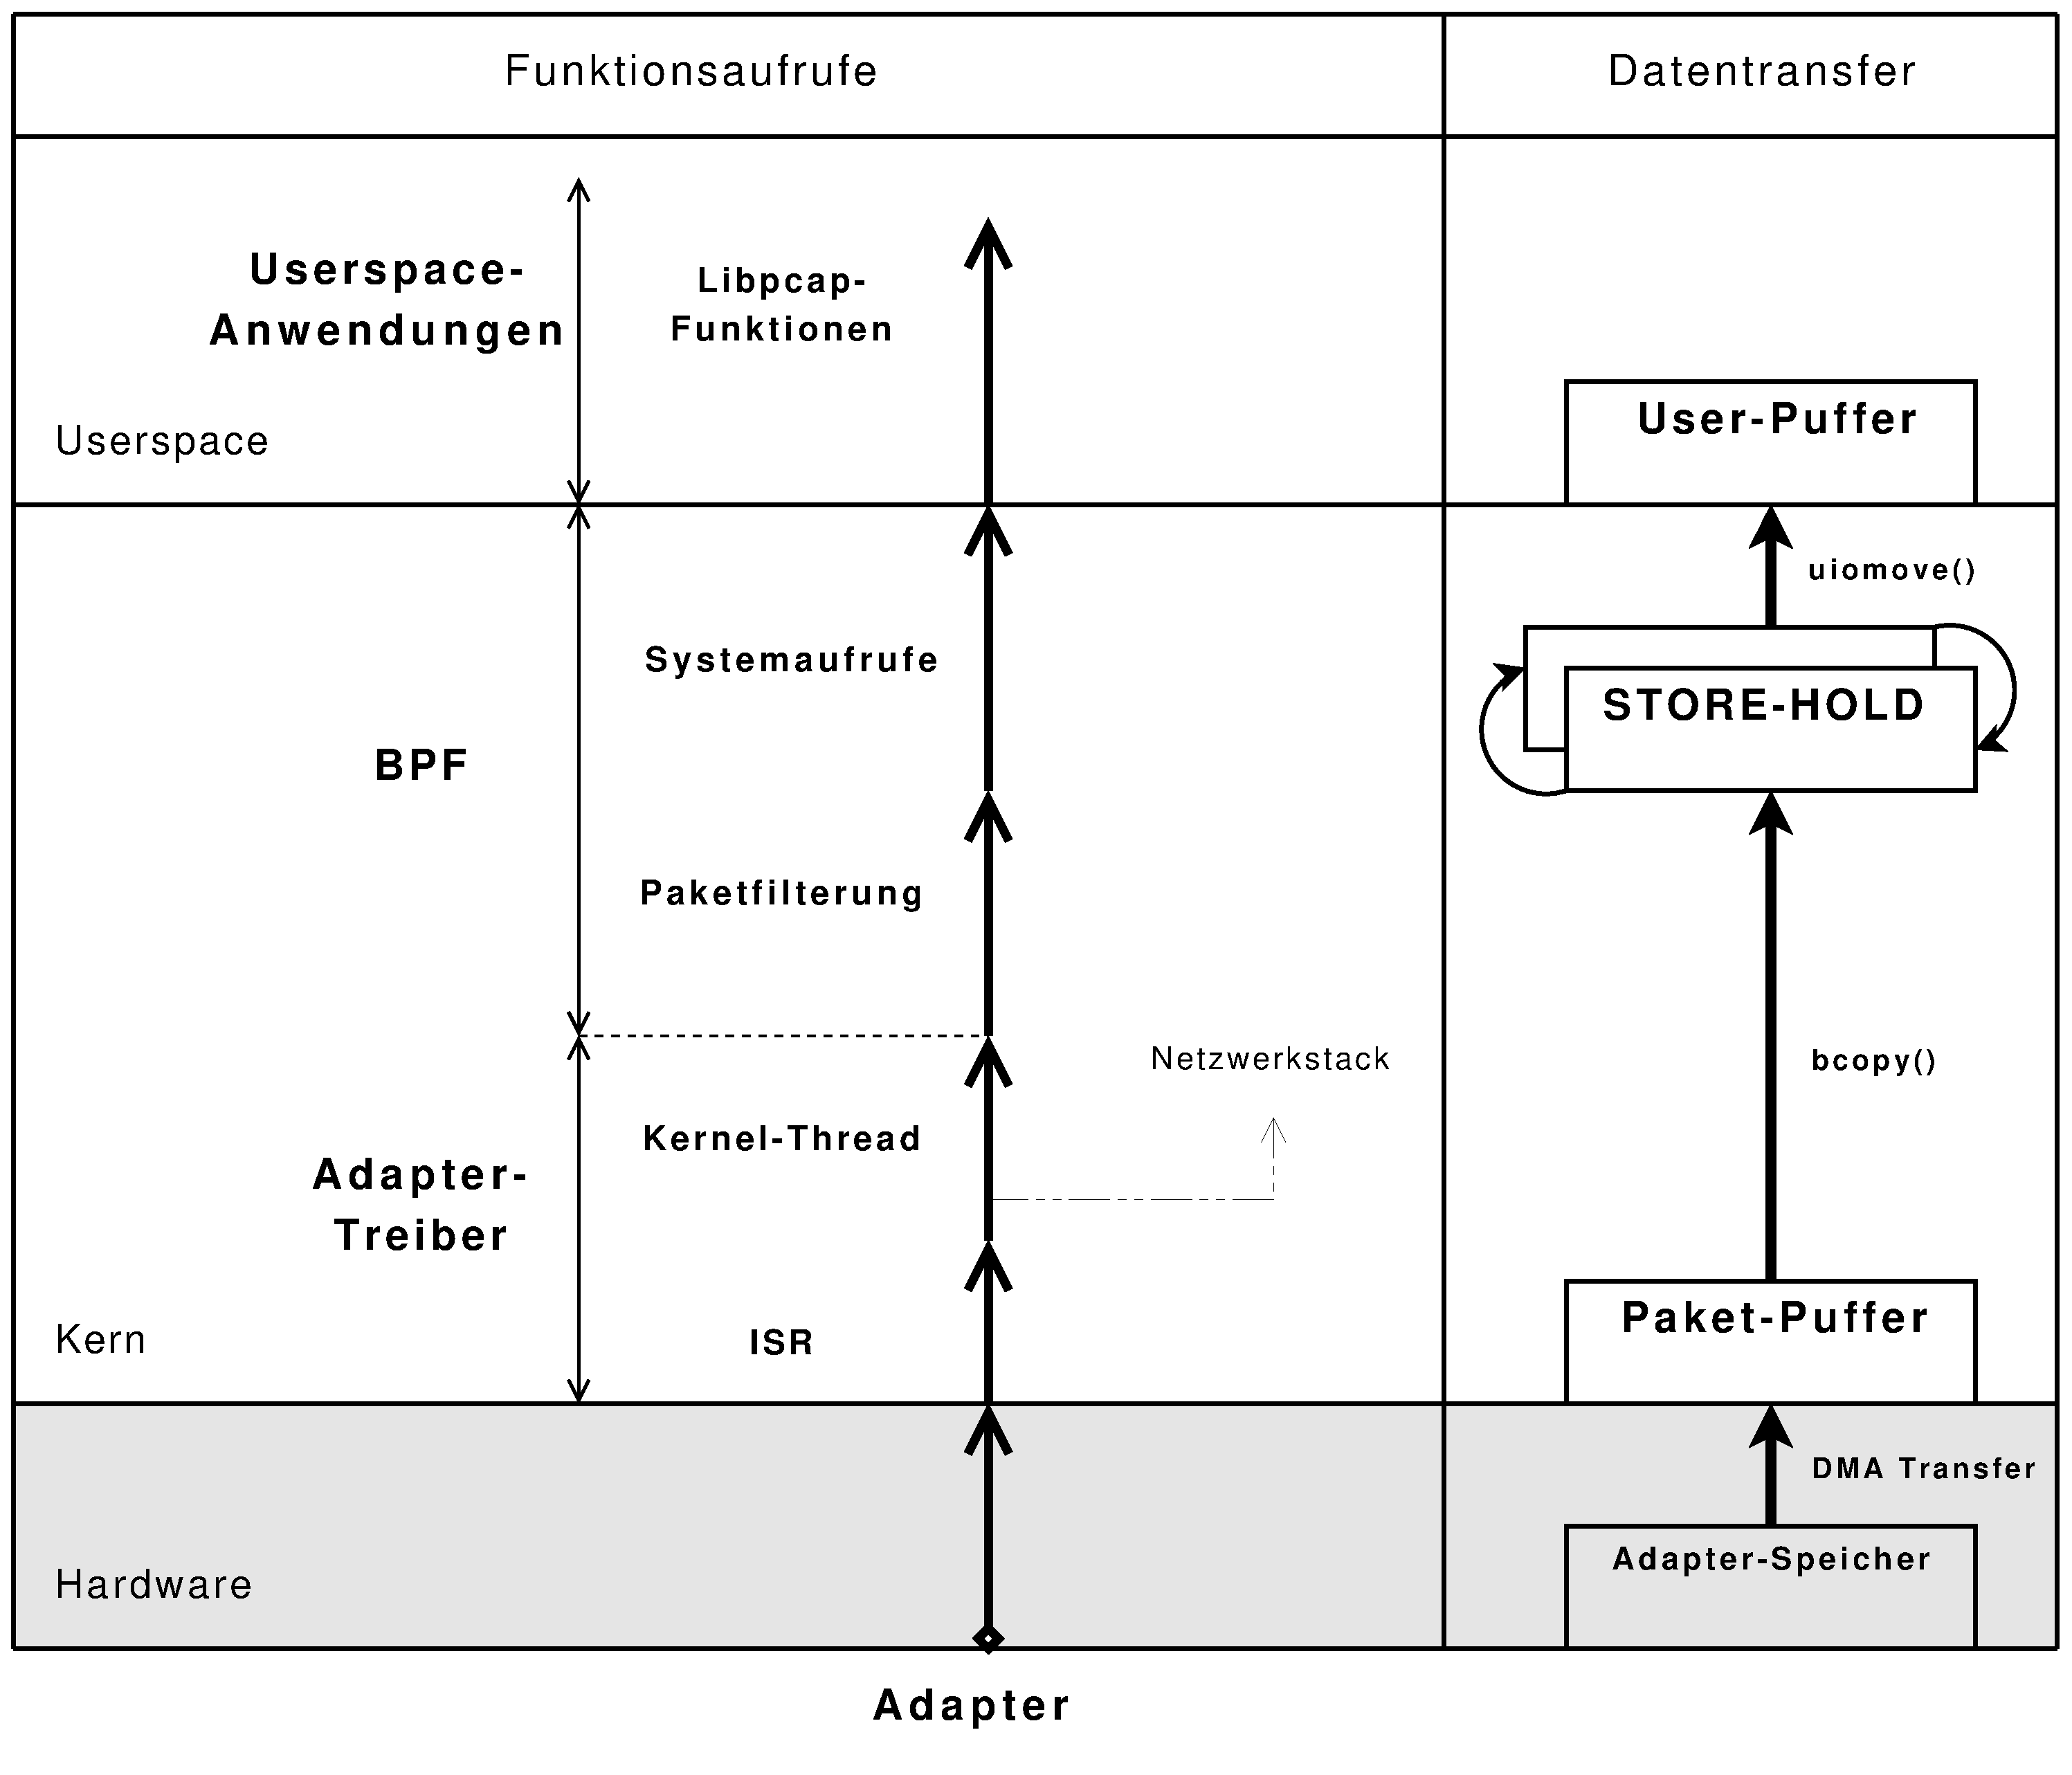
\includegraphics[width=5.1in]{bilder/3copy}
\caption{FreeBSD Packet Capturing Stack}
\label{bsd_cap_stack}
\end{figure}
%
\subsubsection{Interruptbehandlung}\label{sec:intr_behandlung}
Die erste Komponente des Packet-Capturing Stacks (siehe Abbildung
\ref{bsd_cap_stack}) ist der Netzwerk-Treiber. Für jedes empfangene Packet wird
einen neuen Paket-Puffer alloziert. Nachdem ein Paket vom Netzwerk-Adapter in
den Paket-Puffer im RAM kopiert wurde, meldet der Adapter die Anwesenheit von
neuen Daten im RAM durch ein Interrupt, und verursacht damit den Aufruf der
\emph{Interrupt-Service-Routine} (ISR).\\\\ 
%
Da die Interruptbehandlung mit der höchste Priorität ausgeführt wird, sind alle
derzeit laufenden Prozesse auf der aktuellen CPU unterbrochen. Dies kann das
Capturing-Performance negativ beeinflussen, wenn die Interruptbehandlung zu
große  Ausführungszeit hat. Die andere Software-Komponenten, die auf die
empfangene Pakete zugreifen wollen, können in dem Fall nicht genügend
CPU-Zyklen bekommen, denn sie mit der geringeren Priorität ausgeführt sind.
Dies würde zu den vollen Paket-Puffer und als Ergebnis zu den Paketverlusten
führen~\cite{elim_recv_lock}. Deshalb ist es für die Vermeidung von
Paketverlusten sehr wichtig, dass die Interruptbehandlung-Funktionen effizient
implementiert sind und dadurch möglichst kurze Ausführungszeiten haben.\\\\
%
Die Interruptbehandlung wird in zwei Phasen ausgeführt: die eigentliche ISR und
\emph{delayed-ISR}. Die ISR dient nur zum Herausfinden der Ursache des
Interrupts und Planen der delayed-ISR. Die größte Rechenaufwand bei der
Interruptbehandlung findet während der Ausführung des \emph{delayed-ISR}
(Kernel-Thread) statt. Von allen Aufgaben, die der \emph{delayed-ISR} erledigt,
sind die Speicher-Allozierungen, wahrscheinlich, diejenigen die den Großteil
der CPU-Zeit beanspruchen. Während des Paket-Empfangs wird im Kontext von
\emph{delayed-ISR} für jedes empfangene Paket einen neuen Paket-Puffer
alloziert. Dies rettet die bevor empfangene Pakete von Überschreibung hat aber
einen Nachteil, der sich in Vergrößerung des pro-Paket Overhead zeigt,
denn Speicherallozierung ist relativ ``teure'' Operation.
%
\ifthenelse{\boolean{BRIEF}}{}{
%
\begin{figure}
\centering 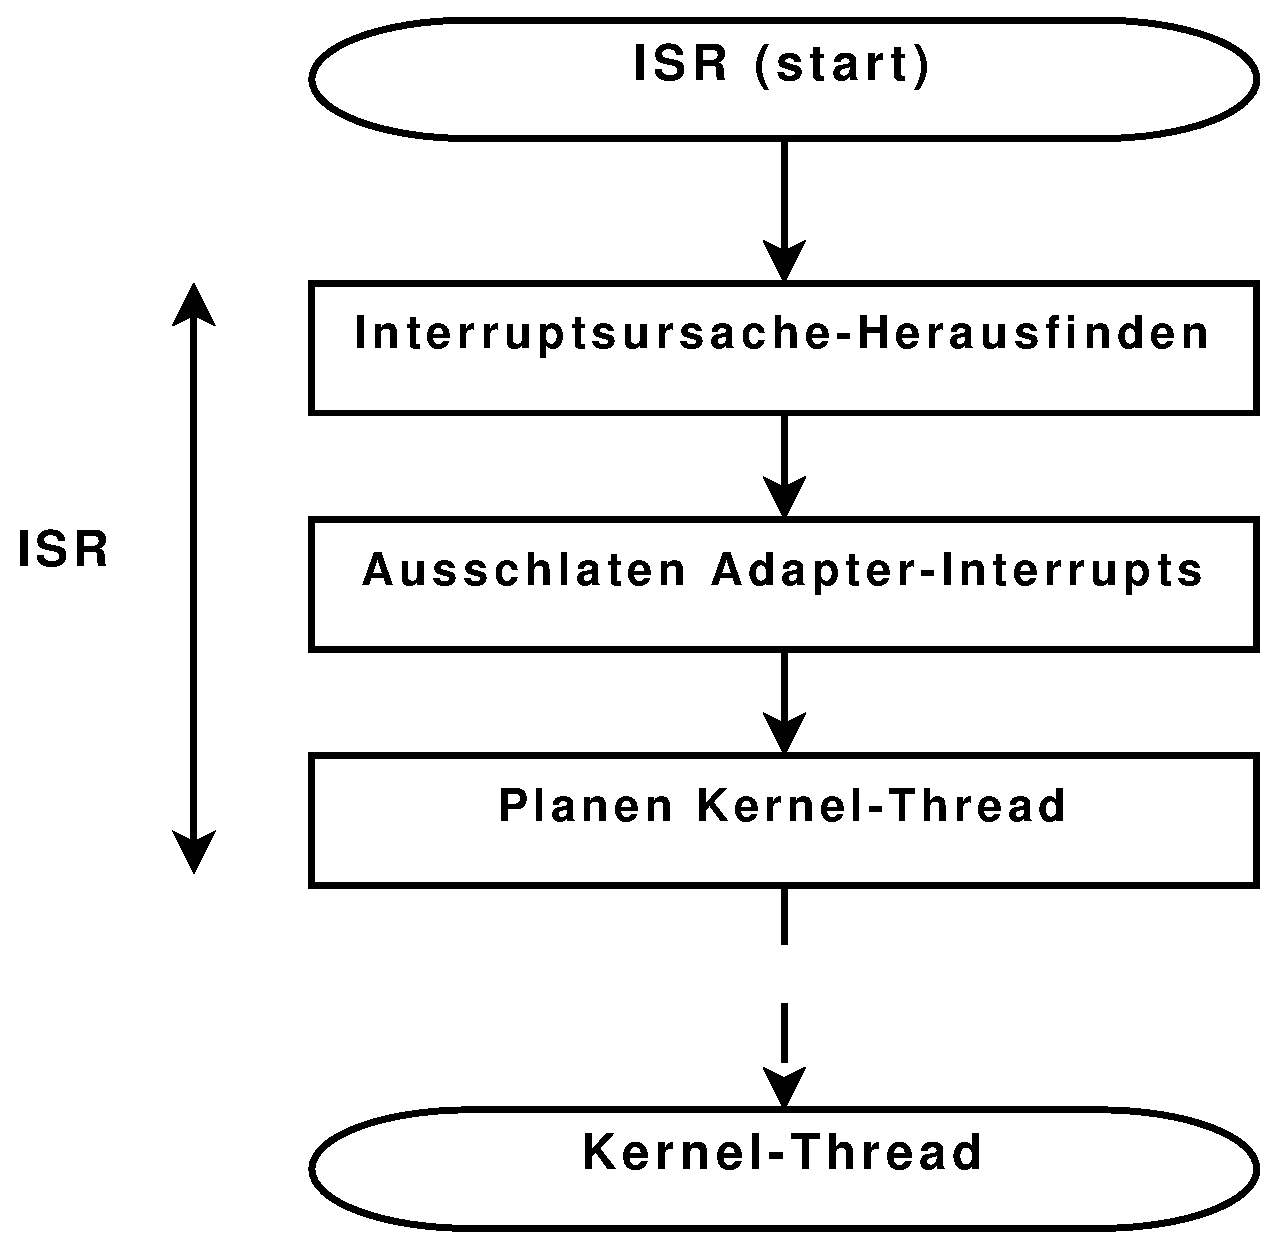
\includegraphics[width=2.0in]{bilder/FlowChart_ISR}
\caption{Adapter-Treiber: Interrupt Service Routine}
\label{img:isr_treiber}
\end{figure}
%
\subsubsection*{Trennung des Interrupt-Handlers in zwei Teile: ISR und Kernel-Thread}\label{sec:intr_isr_kthr}
Da es nicht immer möglich ist, die Ausführungszeit einer ISR zu minimieren,
kann man in ~FreeBSD den Interrupthandler in zwei Teile trennen
~\cite{freebsd_design}.  Der erste Teil ist die eigentliche ISR\footnote{Wird
auch oft in der Literatur als \emph{Fast Interrupt handler} oder \emph{top-half
of interrupt} genannt~\cite{ldd_book}.}, deren Ausführung das Sperren aller
anderen Aktivitäten auf der aktuellen CPU verursacht. Der andere Teil ist ein
Kernel-Thread\footnote{wird auch als \emph{NON-Fast Interrupt handler} oder
\emph{down-half of interrupt} genannt~\cite{ldd_book}.}, dessen Ausführung mit  etwas
niedrigerer Priorität zu einem späteren Zeitpunkt stattfindet (siehe Abbildung
\ref{img:isr_treiber}).\\\\
%
Die ISR des \textbf{em}-Treibers hat  lediglich die Aufgabe durch das Lesen des
\verb+Interrupt-Cause+-Registers (\verb+ICR+)~\cite{e1000_sdm} die Interrupt-Ursache herauszufinden,
die Interrupts des Adapters auszuschalten und die Ausführung eines Kernel-Threads
für die weitere Paketbearbeitung zu planen(siehe Abbildung
\ref{img:isr_treiber}).\\\\
%
Die Aufgabe des Kernel-Threads ist es, die neue durch DMA in die Paket-Puffer
geschrieben Pakete zu lesen, diese auf Fehler zu prüfen, in
\verb+mbuf+-Strukturen~\cite{man_kernel_mbuf, freebsd_design} einzupacken und
dem Protokoll-Stack und BPF zu übergeben (siehe Abbildung
\ref{img:isr_kern_thr}).  Der Kernel-Thread bearbeitet maximal eine bestimmte
Anzahl von Paket-Puffern. Dieser Wert kann über \emph{sysctl}-Befehl
folgender massen gesetzt werden: 
\begin{equation}
			\verb+# sysctl dev.em.0.rx_processing_limit 100+
\end{equation}
Wenn es nach dem Interrupt mehr als \verb+rx_processing_limit+ neue
Paket-Puffer im RAM gibt, wird Kernel-Thread mehrmals geplant. Während des
ersten Ablaufs des Threads sind die Interrupts des Adapter noch gesperrt.  Nach
seinem Ablauf entsperrt der Kernel-Thread die Adapter-Interrupts, sodass die
restlichen Thread-Abläufe mit erlaubten Interrupts stattfinden
und jeder Zeit von neuen
Adapter-Interrupts unterbrochen werden können. Der Grund des Sperrens der
Interrupts nur für den ersten Thread-Ablauf ist nirgendwo beschrieben. Ich
vermute, dass es für dieses Vorgehen folgende Erklärungen gibt: 
\begin{itemize}
	\item Wenn die Interrupts für alle Thread-Abläufe gesperrt wären, könnte
		dann zu lange Inter-Interrupt-Verzögerung entstehen was, den
		Paketverlusten führen würde.
	\item Hätte man vor begin der ersten Thread-Ablauf die Interrupts
		entsperrt, dann könnte bei einer zu hohen Interrupt-Rate dazu kommen, dass der
		Thread ständig durch neue Interrupts unterbrochen würde und dadurch
		nie seine Arbeit erledigt hätte.
\end{itemize}
%
Die Arbeit, die der Kernel-Thread pro Puffer erledigt besteht aus (siehe auch
Abbildung \ref{img:isr_kern_thr}): 
\begin{enumerate}
	\item Allozieren des neuen Paket-Puffer für den aktuellen Deskriptor
	      % \reviewnote{Nenn es eine Variable: P'}
	\item Fehlerprüfung des Paketes im alten Paket-Puffer % \reviewnote{neuer? alter?}
	\item Einpacken des Paketes in \verb+mbuf+-Struktur	
	\item Übergeben des Paketes an den Protokoll-Stack
	\item Übergeben des Paketes an den BPF
	\item Inkrementieren des Wertes in RDT-Register:
		\begin{equation}
			RDT=(RDT+1)\ mod\ SIZE
			\label{form:rdt_inkr}
		\end{equation}
		\emph{SIZE} - Anzahl von Deskriptoren.
\end{enumerate}
\begin{figure}
\centering 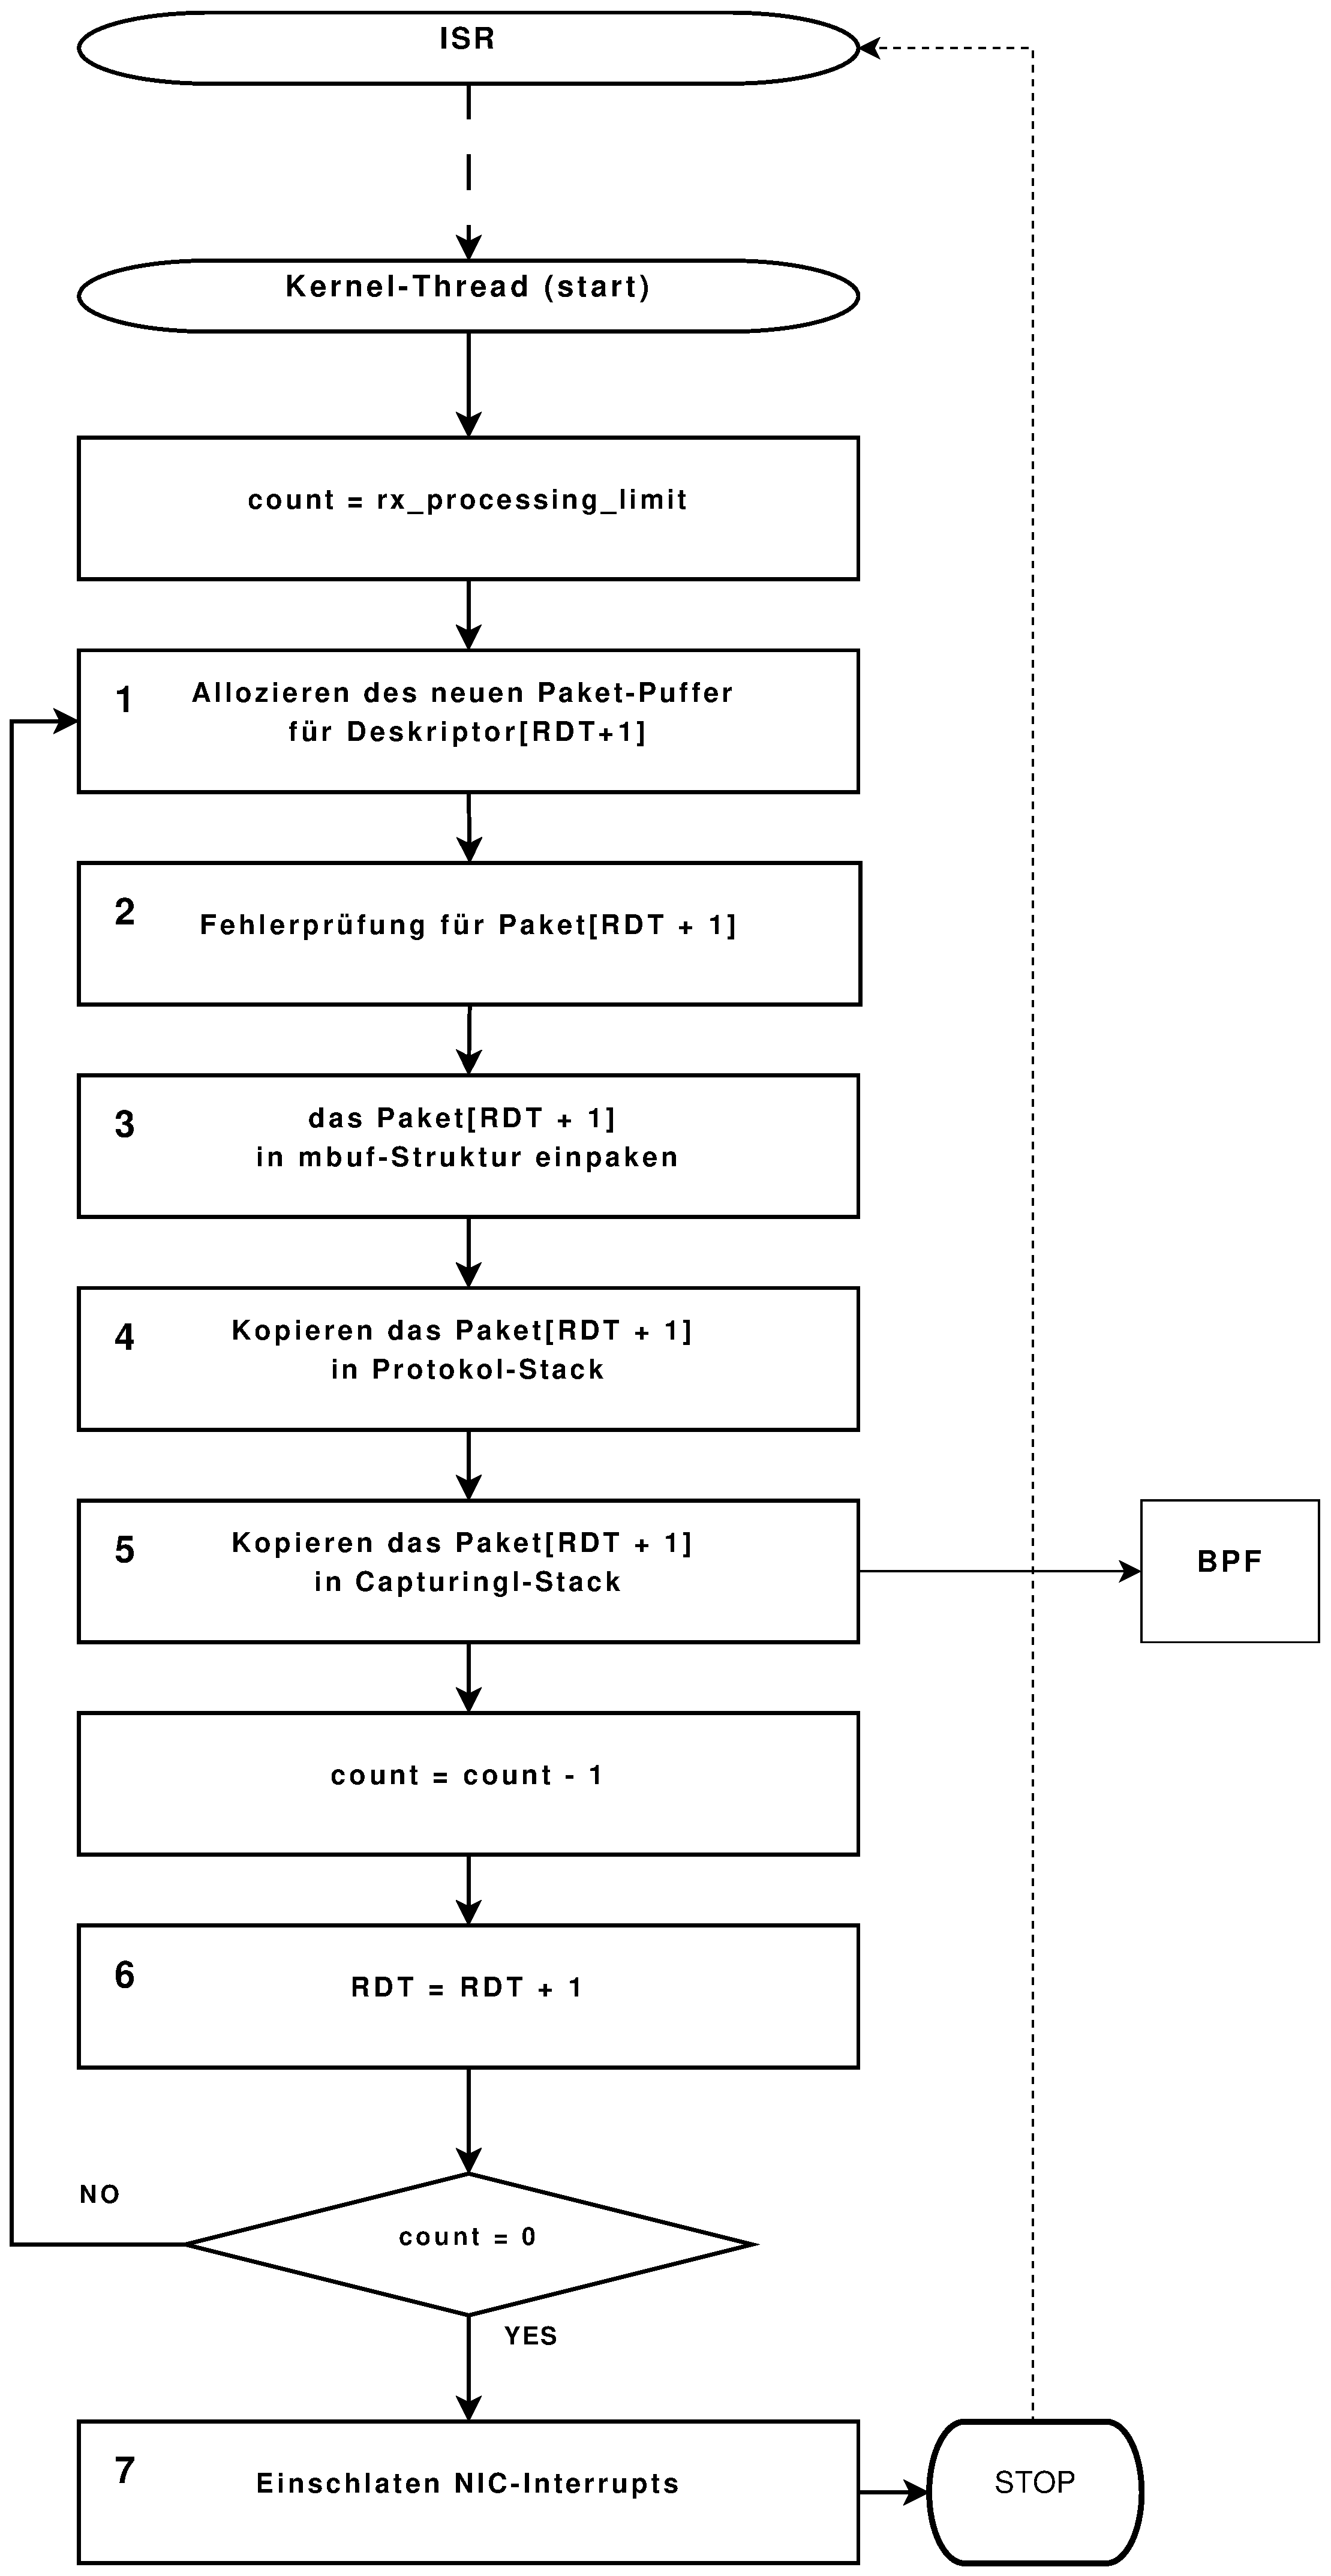
\includegraphics[width=4.5in]{bilder/FlowChart_Kernel_Thread}
\caption{Adapter-Treiber: Kernel-Thread}
\label{img:isr_kern_thr}
\end{figure} 

}
%
\subsubsection{Berkley Packet Filter}\label{sec:bpf}
Der BPF ist die nächste Komponente des FreeBSD Packet-Capturing-Stacks. Der BPF
registriert im System für jeden Prozess, der die Pakete erfassen will ein
symbolisches Device: \verb+/dev/bpf[0-9]+, und bietet dazu eine Menge von
Systemaufrufen (read, ioctl, etc\ldots) für den Zugriff auf die Pakete und zur
Steuerung der Paketfilterung.  Außerdem stellt BPF eine Menge von
Kernel-Funktionen zur Verfügung, die aus dem Treiber aufgerufen werden und die
eigentliche Filterung und Weiterleitung des Paketes durch Capturing-Stack zum
User-Prozess ausführen~\cite{man_kernel_bpf, man_bpf, bpf_paper}.\\\\
%
Die Pakete werden vom BPF gefiltert, und diejenigen, die durch die Filterregeln
akzeptiert wurden, werden in den STORE-HOLD-Puffer kopiert (siehe Abbildung
\ref{bsd_cap_stack}).  Aus dem STORE-HOLD-Puffer werden die Pakete durch den
\emph{read}-Systemaufruf in Userspace übertragen\footnote{Die genaue Beschreibung
ist in \emph{bpf(9)} Manual~\cite{man_kernel_bpf} und in den Papers von Fabian
Schneider~\cite{fabian_da, pcin10gb_paper} zu finden.}.\\\\
%
Der BPF wird auf dem aktuellen FreeBSD vollkommen in Kernelspace ausgeführt.
Es gibt aber auch in der Libpcap-Library eine BPF-Implementierung, was  die
Paketfilterung auch im Userspace erlaubt. Aber das Ausführen von
Filterung-Routinen im Kern, sofort nach dem Paketempfang, hat seine Vorteile.
Die Kopier-Operationen haben mit dem Unterschied zu den anderen wesentlich
längere Ausführungszeiten. Deshalb eliminiert das möglichst frühe Ausführen der
Filterung  das unnötiges Kopieren von Daten, die anhand der vorhandenen
Filterregeln nicht akzeptiert wurden.\\\\
%
Der Performance-Nachteil des klassischen BPF-Models besteht darin, dass es die
``teure'' Paket-Kopier-Operationen im Kernelspace hat und für den Übertragung
der Pakete in den Userspace die Systemaufrufe anfordert, was eine
Kopier-Operation mit dem Ausführung-Kontextwechsel beeinflusst.

\subsubsection{Libpcap}\label{sec:libpcap}
Libpcap ist eine Programm-Bibliothek, die eine Menge von Funktionen zum
bequemen Zugriff auf empfangene Pakete anbietet~\cite{man_pcap}. Mehrere
bekannte Sniffer wie \emph{tcpdump} oder \emph{Wireshark} benutzen Libpcap für
Packet-Capturing.  Auf FreeBSD benutzen die Libpcap-Funktionen  selber
BPF-Systemaufrufe für die Paketfilterung und für Zugriff auf gefilterte Pakete,
und stellen den User-Anwendungen eine bequeme und einfache Schnittstelle für
Capturing.\\\\
%
Während Packet-Capturing sind die Aufgaben der Libpcap-Funktionen, die Pakete in den
Userspace zu holen und den Anwendungen, die auf die Pakete zugreifen wollen einen
Pointer auf Paketpuffer zu übergeben. Dabei besteht keinen großen Overhead, der 
sich deutlich reduzieren lässt. 

\subsection{Capturing-Analyse und Entwurf-Anforderungen}\label{sec:aufgstel}
In den vorherigen Abschnitten wurden die für Capturing-Performance relevanten
Software-Eigenschaften dargestellt. Dabei wurde versucht herauszufinden, welche
der vorgestellten Komponenten unter welchen Umständen die Performance des
Capturing negativ beeinflussen können. In diesem Abschnitt wird anhand der
herausgefundenen Capturing-Performance-Problemen die konkrete Anforderungen am
Entwurf gestellt.
%
\ifthenelse{\boolean{BRIEF}}{}{
Die Hardware-Komponenten eines Capturing-Systems stellen die höchste
theoretische Grenze für die Capturing-Performance dar. Wir haben aber gesehen, dass
in der Realität die Performance bei der Datenbearbeitung wesentlich schlechter
als die theoretischen Werte sein kann. Das kann man z.B. besonders gut beim
Vergleich der theoretischen~\cite{lodb_wiki} und
effektiven~\cite{steram_results_for_pc} Speicher-Bandbreiten sehen.  Einer der
Gründen dafür ist es, das die Software ineffizient die zur Verfügung stehenden
Hardware-Ressourcen nutzt.\\\\ 
%
Aufgrund der Unmöglichkeit der Verbesserung von Hardware-Komponenten im Rahmen 
einer Diplomarbeit und einer relativen Einfachheit der Software-Lösungen 
hat sich für den praktischen Teil der Diplomarbeit die Softwarebasierende 
Lösung entwickelt. Wir wollen einen neuen Paket-Capturing-Stack implementieren, 
in dem möglichst alle in dem aktuellen Stack gefundene Performance-Probleme 
eliminiert werden.\\\\
%
For allem handelt es sich um die Eliminierung der Kopie-Operationen und
Beseitigung des Systemaufrufes für den Datenzugriff, denn genau diese
Funktionen sind es, die im Vergleich zu den anderen Funktionen, eine relativ große
Ausführungszeit anfordern. Das kann mit dem Memory-Mapping gemacht werden.
Dafür muss aber einen Konzept für den Zugriff auf Daten,  die im ``gemappten''
Puffer liegen, erarbeitet werden.
}
%
\subsubsection{Capturing-Stack-Analyse}
Betrachten wir noch mal den in Abbildung\ref{bsd_cap_stack} dargestellten
Capturing-Stack des aktuellen FreeBSD. Stellen wir uns den Fall vor wenn alle
Pakete durch die BPF-Filterung akzeptiert wurden. Dann haben wir pro Paket drei
Kopier-Operationen:
\begin{enumerate}
\item DMA Transfer in den RAM
	\begin{itemize}
		\item ist mit Hilfe der Hardware erledigt
	\end{itemize}
\item Kopieren in STORE-HOLD-Puffer
	\begin{itemize}
		\item ist mit Hilfe der Kernelfunktion \verb+bcopy(9)+ gemacht. 
	\end{itemize}
\item Kopieren in Userspace (mit dem Kontextwechsel)
	\begin{itemize}
		\item ist durch den Systemaufruf \emph{read(2)} erledigt. Dazu 
			Ausführungskontext-Wechsel
	\end{itemize}
\end{enumerate}
Die erste Kopier-Operation, die durch DMA-Transfer erledigt wird, ist
unvermeidlich. Die restlichen zwei Kopier-Operationen und der Kontext-Wechsel
stellen ein Flaschenhals im Capturing-System, falls die Rate der ankommenden
Pakete nah zu $1GBit/sec$ oder höher steigt (siehe Ergebnisse).  Außerdem,
vergrössert das ständige Allozieren der neuen Paket-Puffer im Interrupt-Kontext
den Overhead beim Empfang der Pakete.\\\\
%
Die Kopier-Operationen lassen sich durch die Memory-Mapping eliminieren. Wenn
die Paket-Puffer in den Address-Raum einer Capturing-Anwendung eingeblendet
werden, dann braucht diese Anwendung keine Kopier-Operationen und keine
Systemaufrufe mehr, um die Pakete zugreifen zu können. Dafür muss aber ein 
Synchronisation-Verfahren erarbeitet werden, wenn die mehrere Prozesse auf 
den gleichen Paket-Puffer zugreifen werden.\\\\
%
Die Speicherallozierungen lassen sich durch die Anwendung von dem Ring-Buffer
ersetzen. Der Ring-Buffer präsentiert eine constante Menge der preallozierten
Speicherbereichen und zwei Zeiger: \emph{HEAD} and \emph{TAIL}. Das Besondere am
Ring-Buffer ist es, dass er eine feste Größe hat und die Speicherbereiche die er
verwaltet, nur ein mal alloziert und dann ein nach einander beschrieben und
gelesen werden. Dabei, zeigt \emph{HEAD} auf den nächsten freien
Speicherbereich, der beschrieben wird. \emph{TAIL} zeigt auf den zuletzt
gelesenen Bereich. Im Unterschied zum normalen Array werden die ältesten Inhalte
überschrieben, wenn der Ring-Buffer voll ist und weitere Elemente in den
Ring-Buffer abgelegt werden.
\subsubsection{Anforderungen für den Entwurf}
\begin{enumerate}
	\item Alle Paket-Kopie-Operationen im Capturing-Stack sollen eliminiert
		werden (Abbildung \ref{img:new_stack})
		\begin{itemize}
			\item Die Pakete sollen sofort nach dem DMA-Transfer im virtuellen 
				Adressraum des User-Capturing-Prozesses zugreifbar sein.
		\end{itemize}
	\item Keine Speicherallozierungen für die neue Paket-Puffer während des Capturing
		\begin{itemize}
			\item Alle Paket-Puffer sollen bei der Initialisierung des Treiber
				alloziert werden und für die ganze Laufzeit des Treibers für
				Empfang der neuen Pakete der Reihe nach benutzt werden.
		\end{itemize}
	\item Keine Systemaufrufe für den Datenzugriff und Paketbearbeitung
		während des Capturing
		\begin{itemize}
			\item Dafür müssen außer den Paket-Puffern noch andere
				Datenstrukturen mit den für das Capturing relevanten Daten in den
				Userspace eingeblendet werden, damit der Userspace-Prozess ohne
				Systemaufrufe die Daten vom Treiber bekommt und auch
				Informationen an den Treiber liefern und damit das Capturing
				steuern kann.
			\item   Systemaufrufe sind nur während der Initialisierung des
				Capturing-Prozesses 
			        % versteh ich nicht, kann auch weg, oder? -- Andi
			        %für das Holen der benötigten Daten vom
				%Adapter in den Userspace,
				und während der Abwesenheit von neuen
				Paketen für das Blockieren des auf die Pakete wartenden
				Prozesses erlaubt. 
		\end{itemize}
%	\item Anpassung der Libpcap zum Zugriff auf Pakete in den ``gemappten'' Puffer
%		\begin{itemize}
%			\item Die Anpassung soll transparent für die Libpcap-Anwendungen sein. 
%		\end{itemize}
	\item Eine Userspace-Capturing-Anwendung pro Netzwerk-Interface
		\begin{itemize}
			\item Wir begrenzen uns auf eine gleichzeitig aktive Userspace-Capturing-Anwendung
			      pro Interface, um den Entwurf und die Implementierung einfach zu halten.
		\end{itemize}
%	\item Ringpuffer-Struktur für den Paketzugriff.
%		\begin{itemize}
%			\item Die Gründe für die Auswahl der Ringpuffer-Struktur für den Datenzugriff 
%				sind im Kapitel Entwurf \ref{sec:Entwurf} erklärt.
%		\end{itemize}
	\item Protokoll-Stack ausschalten 
		\begin{itemize}
			\item Wir wollen den neuen Treiber nur für Capturing benutzen
		\end{itemize}
	\item BPF aus dem Kernel entfernen. 
		\begin{itemize}
			\item Der BPF ist auch in der Libpcap implementiert. Das hat zur Folge, dass
				es kein Problem wäre, die Paketfilterung im Userspace anzuwenden.
		\end{itemize}
\end{enumerate}
Da der neue Stack anders als der Standard-FreeBSD-Capturing-Stack die empfangene Pakete den
Userspace-Prozessen zur Verfügung stellt, müssen die Userspace-Prozesse anders
auf die Pakete zugreifen. Um der neue Stack einsetzbar zu machen soll am besten
die Libpcap-Library für ihn angepasst werden, sodass für alle
Capturing-Anwendungen, die auf Libpcap basieren, keine Änderungen benötigt
werden. 

\subsubsection{Namenskonventionen}
Um die Unverständlichkeiten mit den Bezeichnungen zu vermeiden, geben wir 
hier die Namen, unter denen die standard FreeBSD-Capturing-Stack und 
der neuen im Rahmen der Diplomarbeit entwickelten Capturing-Stack in den 
Weiteren Abschnitten auftauchen werden: 
\begin{description}
	\item[ringmap]: Wird als Bezeichnung für die im Rahmen der Diplomarbeit 
		entwickelte Capturing-Software benutzt. 
	\item [generic]: Wird als Bezeichnung für die FreeBSD-\textbf{7.x}-Standard-
		Capturing-Software benutzt.
\end{description}


\begin{figure}
	\begin{center}
	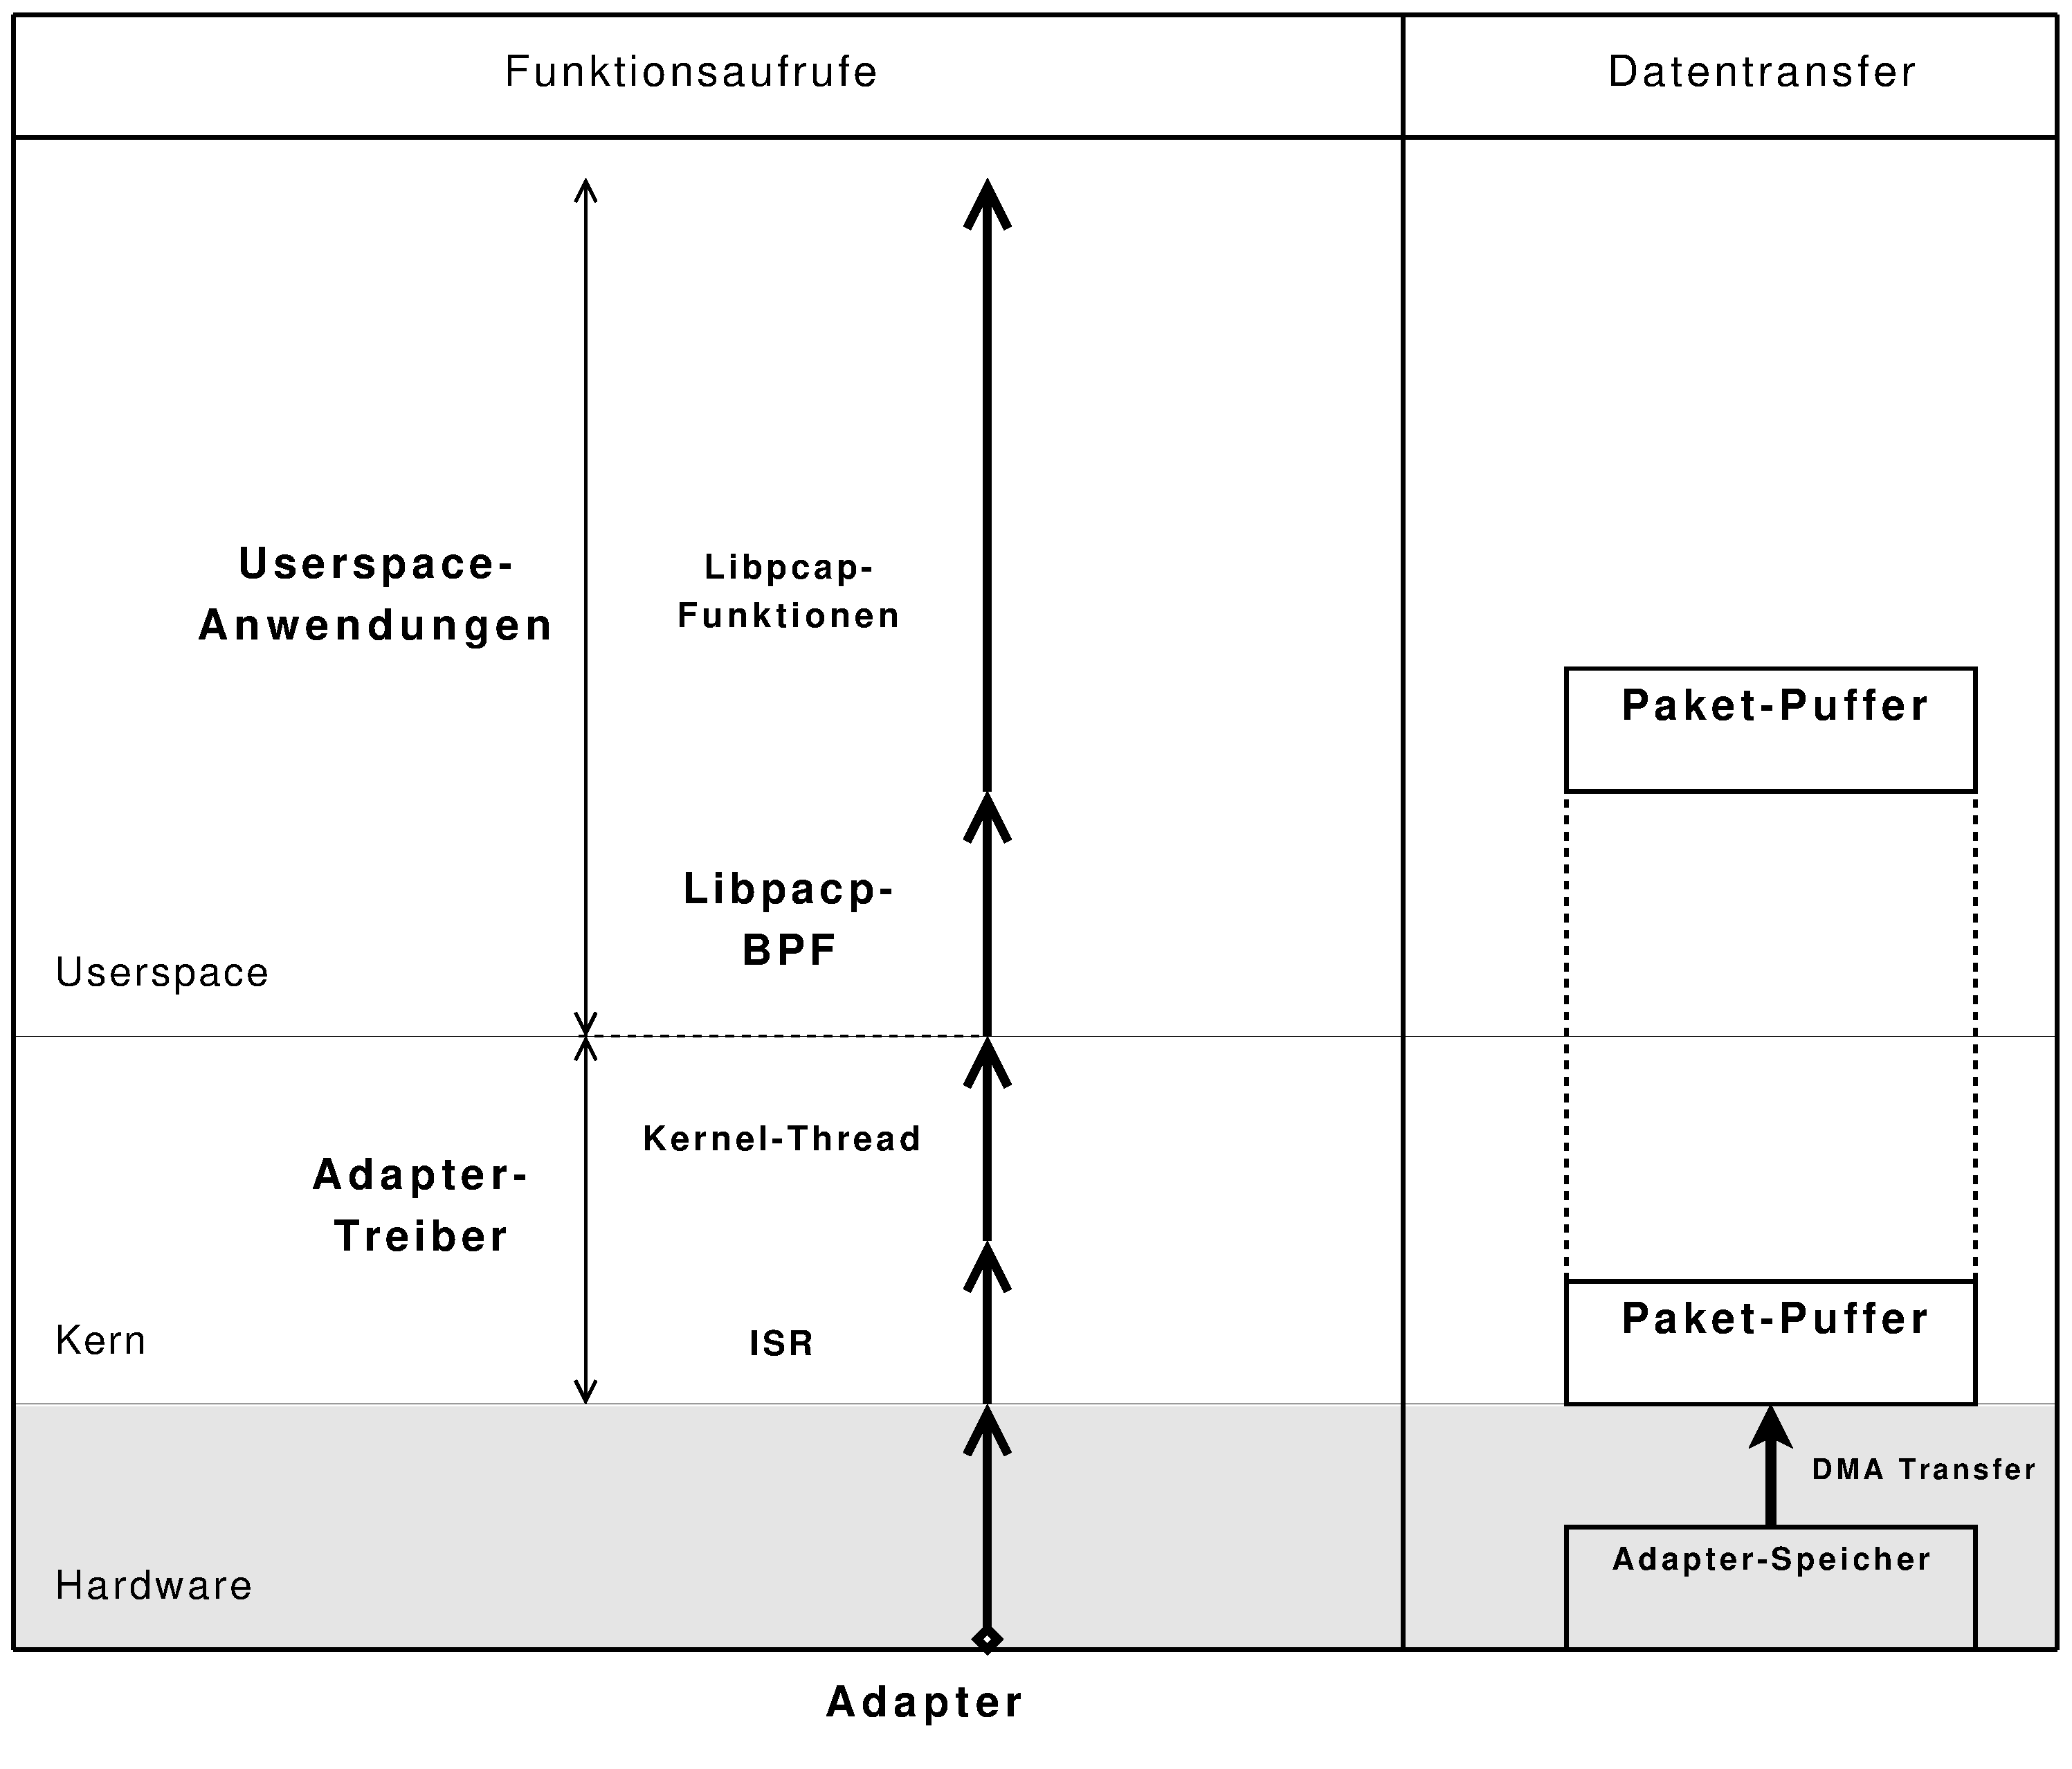
\includegraphics[width=4.9in]{bilder/1copy}
	\end{center}
	\caption{Der neue ringmap-Capturing-Stack. Ziel der Diplomarbeit}
	\label{img:new_stack}
\end{figure}

\ifthenelse{\boolean{BRIEF}}{}{
\subsection{Zusammenfassung}
In diesem Kapitel wurden die für das Verständnis der Capturing-Problematik
relevanten Hintergründe dargestellt. Es wurden sowohl die Software- als auch
die Hardware-Aspekte, welche die Capturing-Performance beeinflussen können,
betrachtet und analysiert. Die Hardware-Eigenschaften eines Capturing-System
sind deshalb wichtig, weil für die Diplomarbeit eine konkrete  Hardware
vorausgesetzt wurde (siehe Abschnitt \ref{sec:hwsw_voraus}), und die
Problemlösung für das Erreichen der maximalen Capturing-Performance
Hardware-Abhängig sein dürfte.\\\\
Außerdem es wurden einige Hardware-Eigenschaften erläutert die zwar keinen
Einfluss auf die Implementierung des neuen Paket-Capturing-Stack haben, 
aber vom Benutzer des Betriebssystem geändert werden können und dadurch die
Capturing-Performance beeinflussen. Es handelt sich dabei um
\emph{Interrupt-Coalescing} (Abschnitt \ref{sec:intr_coal}) und
\emph{Prozessoraffinität} (Abschnitt \ref{sec:cpu_einfl_auf_cap}). Die
Notwendigkeit diese Eigenschaften zu kennen liegt darin, dass sie unabhängig
von Effizienz der Implementierung der Capturing-Software die
Capturing-Performance beeinflussen und dadurch bei ungünstigen Einstellungen
reduzieren können.\\\\
%
Beim Betrachten der unterschiedlichen Hardware- und Software-Komponenten wurde
auch analysiert unter welchen Umständen Engstellen beim Capturing auftreten
können, und anhand der herausgestellten Problemen wurden die Anforderungen für
den praktischen Teil der Diplomarbeit definiert (Abschnitt
\ref{sec:aufgstel}).\\\\ 
%
Das Ziel des praktischen Teiles der Diplomarbeit ist die Implementierung eines
neuen Capturing-Stacks für das Betriebssystem FreeBSD. Dafür soll eine neue
Software implementiert werden, deren Aufgaben es ist, die gefundenen
Engstellen, die bei der Bearbeitung der im RAM liegenden Pakete entstehen
können, zu beseitigen. Es handelt sich vor allem um die Kopier-Operationen und
die Systemaufrufe, die bei Paket-Filterung oder beim Paket-Zugriff verwendet
werden. \\\\
%
Die Capturing-Performance-Probleme die während der Speicherung der Pakete auf
die Festplatte und der Darstellung der Pakete auf dem Terminal auftreten können wurden nicht
Betrachtet und sind nicht Gegenstand dieser Arbeit.
}

\newpage

\section{Entwurf}\label{sec:Entwurf}
In diesem Kapitel werden die Datenstrukturen und Algorithmen des neuen im
Rahmen der Diplomarbeit entwickelten ringmap-Packet-Capturing-Stack für
Betriebssystem FreeBSD dargestellt. Das Ziel des Entwurfes war einen neuen
Capturing-Stack mit verbesserter Performance zu erarbeiten. Dafür wurden
durch Analyse im Kapitel \ref{sec:aufgstel} die Probleme des aktuellen
generic-Capturing-Stack herausgestellt. Anhand der gefundenen Probleme
wurden die Anforderungen für den neuen ringmap-Stack, mit dem Ziel den
Datendurchstz beim Capturing zu erhöhen, erstellt.\\\\
%
\subsection{Datenstrukturen}
Die im \emph{ringmap}-Capturing-Stack verwendete Daten-Strukturen dienen zur Modellierung
aller für Paketempfang verantwortlichen Paket-Puffer in Form  eines
Ringpuffers. Die Gründe für die Auswahl der Ringpuffer-Struktur sind in
folgenden Abschnitten dargestellt. Der Stacks sind für die
Paketzustellung und den Paketzugriff im Ringpuffer und auch für die Steuerung
des Capturing-Prozesses zuständig.

\subsubsection{Verwendungszwecke für Ringpuffer}
Die Ringpuffer-Daten-Struktur wird bevorzugt wenn es um den Datenzugriff in
einem Array oder einer Liste handelt, bei der die Elementenanzahl konstant bleiben
soll und neue Speicherallozierungen unerwünscht wären. Darüberhinaus werden
Ringpuffer für die Lösung einiger klassischen Problemen, z.B.
Erzeuger-Verbraucher-Problem~\cite{erz_verbr_wiki},
empfohlen~\cite{ldd_book_circle_buffer}.

\subsubsection{Gründe für die Ringpuffer-Struktur im ringmap-Capturing-Stack}
Die Gründe für die Auswahl der Ringpuffer-Struktur für den Paket-Capturing
basieren vor allem auf den im Kapitel \ref{sec:aufgstel} für den 
\emph{ringmap}-Capturing-Stack gestellten Anforderungen (Anforderungen \textbf{1.} und
\textbf{2.}). Außerdem spielen für die Auswahl der Ringstruktur auch die
andere folgende Faktoren und die Hardware-Eigenschaften eine wichtige Role:
\begin{itemize}
	\item Der Capturing-Prozess ist dem
		Erzeuger-Verbraucher-Modell~\cite{erz_verbr_wiki} ähnlich:
		\begin{itemize}
			\item Es gibt ein ``Datenerzeuger'': der Netzwerkadapter-Treiber, der die
				Pakete in den Ringpuffer für folgende Bearbeitung bzw.
				Filterung vorbereitet.
			\item Es gibt  ein ``Datenverbraucher'': die User-Anwendung, die
				auf die in den Paket-Puffer befindlichen Pakete zugreift,
				sie bearbeitet, speichert oder darstellt.
		\end{itemize}
	\item Der Netzwerkadapter verwaltet die Deskriptoren als ein Ringpuffer (siehe
		Abschnitt \ref{sec:adapter}).  Der Netzwerkadapter enthält die
		\verb+RDT+- und \verb+RDH+-Register, welche die Role der HEAD und
		TAIL-Pointers im Deskriptor-Ringpuffer speilen und dadurch, dass jeder
		Deskriptor einen Paket-Puffer referenziert, können diese Register auch
		als HEAD und TAIL für den Paket-Puffer-Array nützlich sein.
\end{itemize}

\subsubsection{Memory-mapped Paket-Ringpuffer für ringmap-Capturing-Stack}\label{sec:memmap_pr}
Alle Paket-Puffer werden in den Adressraum eines Capturing-Prozesses
eingeblendet, damit der Capturing-Prozess ohne Kopie-Operationen und ohne
Systemaufruf auf die Pakete zugreifen kann. Mit jedem Paket-Puffer werden zwei
weitere Daten-Strukturen in den Userspace eingeblendet. Das sind
\verb+mbuf+~\cite{man_bpf} und Deskriptor.  Diese Strukturen werden im Userspace
deshalb gebraucht, weil sie die für Paketbearbeitung und Paketfilterung
relevante Informationen enthalten.  Auf diese obengenannten Datenstrukturen
wird sowohl vom Kernelspace als auch vom Userspace zugegriffen.  Um dies zu
ermöglichen werden drei andere Datenstrukturen zur Adressierung vorgesehen, 
welche sowohl die Kernelspace- als auch die Userspace-Adressen von den 
Paket-Puffer, \verb+mbuf+'s und Deskriptoren enthalten.
Das sind: \verb+PAKET+, \verb+MBUF+ und  \verb+DESKRIPTOR+ (siehe Abbildung
\ref{img:uml_ring}).\\\\
%
Jedes Paket im RAM wird durch den Tripel \verb+[PAKET, MBUF, DESKRIPTOR]+
repräsentiert. Jedes Tripel wird in einer Datenstruktur \verb+RING_SLOT+
gekapselt.  Und die Instanzen von \verb+RING_SLOT+ bilden ein Array,
der in der \verb+RING+-Struktur enthalten ist.  Die \verb+RING_SLOT+-Struktur
enthält unter anderem die Platzhalter für \verb+Timestamp+ und \verb+Counter+
vom repräsentierten Paket.\\\\
%
\verb+RING+-Struktur enthält den Array von \verb+RING_SLOT+-Instanzen und die
\verb+HEAD-+ und \verb+TAIL+-Pointers, welche die \verb+HEAD-+ und
\verb+TAIL-+Slots im \verb+RING_SLOT+-Array referenzieren. Damit bildet
\verb+RING+ eine Datenstruktur die es erlaubt, alle  Paket-Puffer als ein
Ringpuffer zu betreiben.\\\\
%
Die \verb+RING+-Struktur wird mit den Paket-Puffer in den Adressraum eines
Userspace-Capturing-Prozesses eingeblendet, und erlaubt ihm den Zugriff auf alle
Paket-Puffer und das Betreiben aller Paket-Puffer als ein Ringpuffer.
%
\begin{figure}
\centering 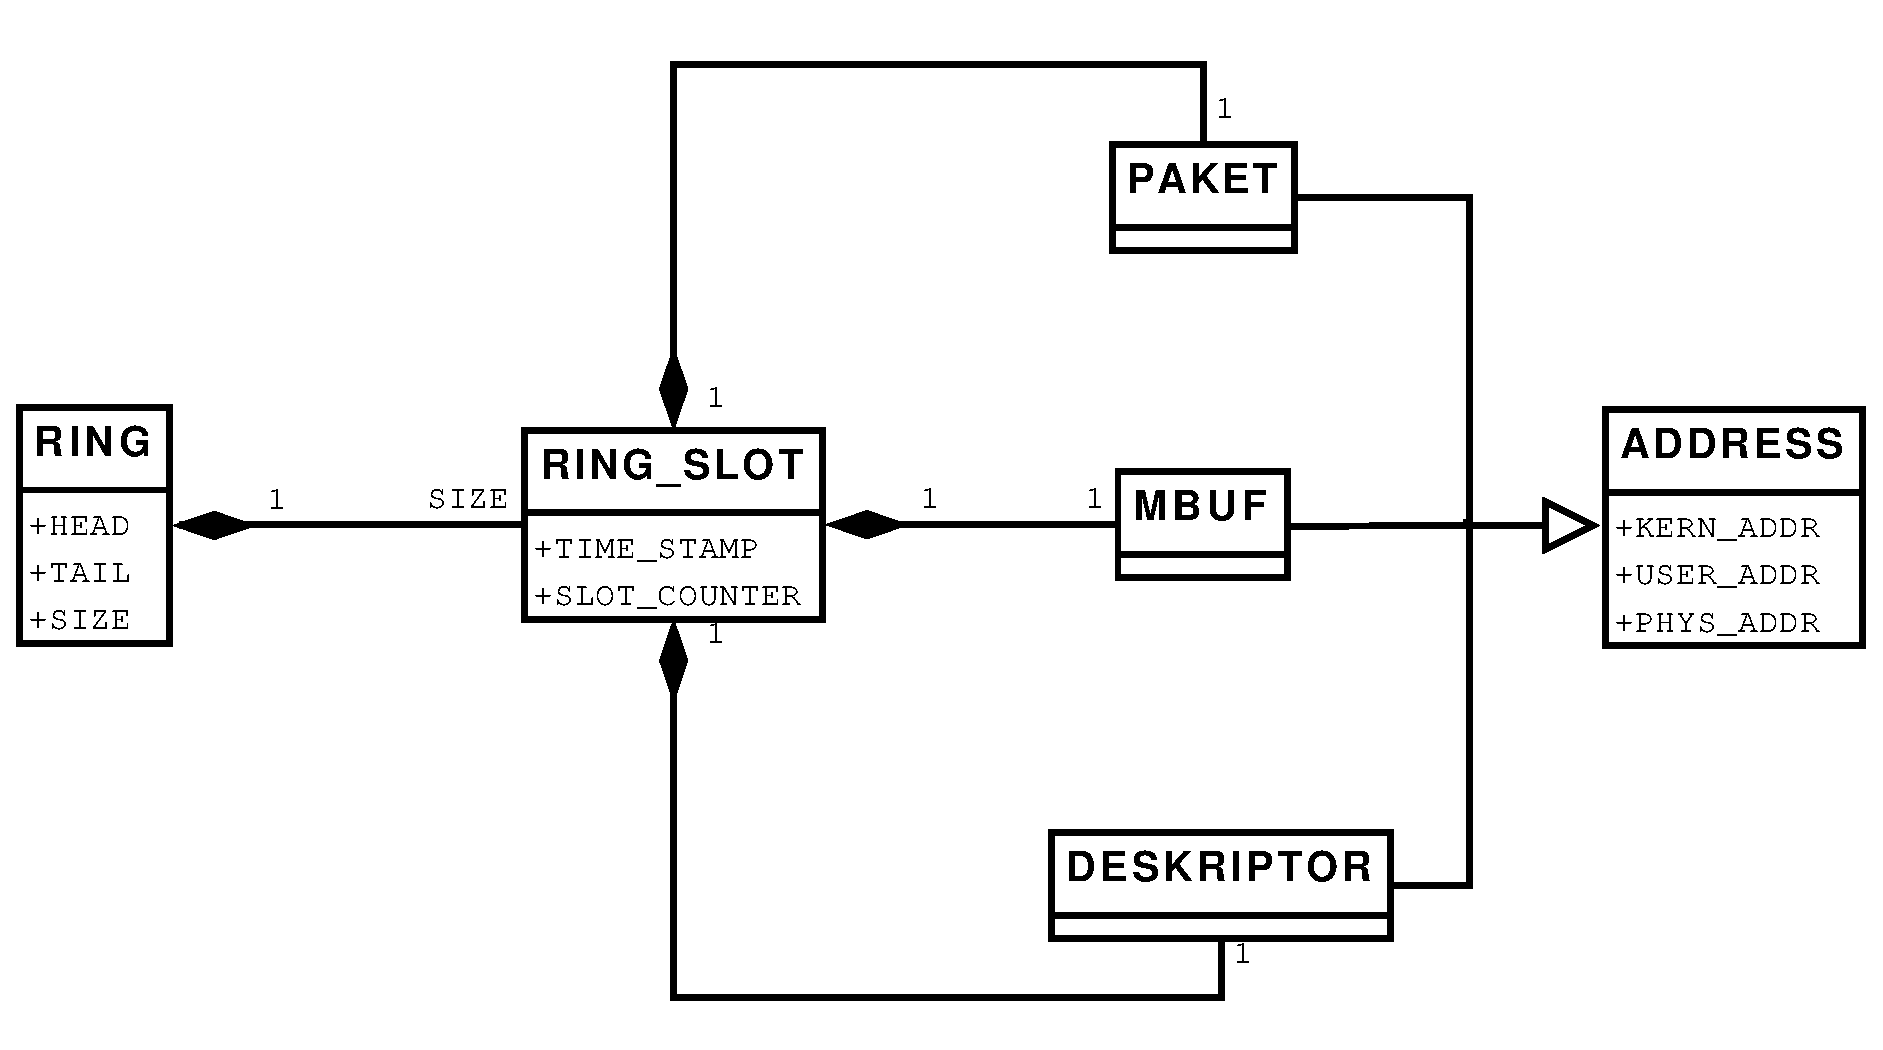
\includegraphics[width=6.4in]{bilder/uml_RING_Puffer}
\caption{Datenstrukturen des Ringpuffer}
\label{img:uml_ring}
\end{figure}

\newpage
\subsection{Funktionalität}
Der neue Capturing-Stack enthält die folgende Funktionalitäten:
\begin{itemize}
	\item \textbf{Paketzustellung}:
		\begin{itemize}
			\item Zustellung der Pakete in den Ringpuffer wird mit Hilfe des
				\textbf{Netzwerkadapter-Treibers} realisiert. 
		\end{itemize}
	\item \textbf{Paketzugriff}:
		\begin{itemize}
			\item  Zugriff auf die im Ringpuffer befindlichen Pakete  wird beim
				\textbf{Userspace-Capturing-Prozesses} gemacht.
		\end{itemize}
	\item \textbf{Systemaufrufe} für:
		\begin{itemize}
			\item Memory-Mapping.
			\item Capturing-Steuerung:  Capturing-Anhalten und -Fortsetzen.
			\item Blockierendes Warten auf neue Pakete.
		\end{itemize}
	\end{itemize}
Aufgrund der Anforderung 4. (siehe Kapitel \ref{sec:aufgstel}), darf
in einem Capturing-Stack nur ein Paketzugriff-Prozess sein. Weil es  nur einen
Zustellung-Prozess (den Treiber) und nur einen Paketzugriff-Prozess gibt,
werden keine \emph{race conditions} beim Zugriff auf Paket-Puffer auftreten,
und dadurch werden keine Synchronisation-Maßnahmen benötigt ~\cite{ldd_book_circle_buffer}.\\\\
%
Nach der Anforderung 3. dürfen während des Ablaufs des Capturing keine
Systemaufrufe auftreten. Gemeint sind die Systemaufrufe die für den Zugriff auf
empfangene Pakete gebraucht wären. Durch \textbf{Memory-Mapping} werden die
Systemaufrufe für den Paketzugriff eliminiert. Es gibt aber die Systemaufrufe
die nicht zu beseitigen sind. Das sind die, welche für die Realisierung vom
\textbf{Memory-Mapping} selbst benötigt werden.  Außerdem wurden auch die Systemaufrufe
für die \textbf{Capturing-Steuerung} und \textbf{blockierendes Warten} auf neue
Pakete implementiert. Theoretisch könnte man die \textbf{Capturing-Steuerung}
durch die Interaktion mit dem Kernelspace über die eingeblendete
Speicherbereiche realisieren. Das \textbf{blockierende Warten} ist auch nicht
die einzige Lösung, wenn der Userspace-Prozess auf die neue Pakete warten soll.
Er kann ja auch aktiv, in einer Schleife, warten.  Das Vermeiden von
Systemaufrufen für die zwei obengenannten Probleme (Capturing-Steuerung und
blockierendes Warten) ist zwar losbar, hat aber einen zusätzlichen Aufwand und
stellt den Performance-Gewinn unter die Frage:
\begin{itemize}
	\item \textbf{Capturing-Steuerung über Shared-Memory}: Wenn der
		Capturing-Prozess nicht über den Systemaufruf, sondern über die
		\emph{Shared-Memory} eine Anfrage an Treiber stellt, soll er darauf
		warten, bis der Treiber-Prozess die CPU für seinen Ablauf bekommt.  Da
		die Funktionen des Treibers, die nicht in folge eines  Systemaufrufes,
		sondern in folge eines  Interrupts aufgerufen werden, in den
		unvorhersagbaren Zeitpunkten stattfinden, kann es dazu führen, dass der
		Capturing-Prozess keine sofortige Reaktion vom Treiber nach seiner
		Anfrage bekommt. Dieses Problem kann mit Hilfe eines
		Kernel-\emph{Watchdog}~\cite{wiki_watchdog} gelost werden, was aber
		nicht nur einen Implementierung-Aufwand mit sich bringt, sondern auch
		den Systemload erhöht.
	\item \textbf{Das aktive Warten auf die neue Pakete}: Das aktive Warten
		beansprucht keinen Systemaufruf dennoch vermeidet das keinen
		Kontextwechsel-Overhead, denn das Betriebssystem blockiert selber im
		Lauf des Prozess-Scheduling den laufenden Prozess um den anderen
		Prozessen die CPU zur Verfügung zu stellen. Außerdem reduziert das
		Betriebssystem die Priorität des aktiv wartenden Prozesses wegen seiner
		ständigen CPU-Nutzung, was die Capturing-Performance negativ
		beeinflussen kann.
\end{itemize}
Jeder Systemaufruf bringt unvermeidlich mit sich einen Overhead (Kontextwechsel
und ggf. Daten-Kopieren) mit sich. Wie kritisch dieser Overhead für
Capturing-Performance ist, hangt von der Häufigkeit des Auftretens der
Situationen, in denen die Systemaufrufe gebraucht werden.  Das
\textbf{Memory-Mapping} im FreeBSD kann nur mit Hilfe eines Systemaufrufes in
die Tat gebracht werden, deshalb für dieses Vorgehen ist der Systemaufruf nicht
zu vermeiden. Die \textbf{Capturing-Steuerung} ist eher ein seltenes Ereignis,
denn es wird ja nicht ständig gebraucht, softwaremässig den Capturing
anzuhalten und fortzusetzen.  Deshalb ist die Verwendung der Systemaufrufen für
Capturing-Steuerung eher unkritisch. Wenn es aber um Warten auf neue Pakete
geht, dann ist aufgrund der unvorhersagbaren Netz-Verkehr das Auftreten des
wartendes Zustandes auch nicht berechenbar ist. Dennoch für das Warten auf neue 
Pakete wird in \emph{ringmap} blockierendes Warten verwendet.
%
In den folgenden Abschnitten werden die Algorithmen der im Capturing-Stack 
beteiligten Funktionalitäten dargestellt.

\subsubsection{Paketzustellung in den Ringpuffer. Netzwerktreiber}
Die Paket-Zustellung in den Ringpuffer wird beim Netzwerkadapter-Treiber
erledigt. Die eigentliche Zustellung macht natürlich der Adapter durch den
DMA-Transfer selbst.  Der Treiber bereitet nur die in den RAM geschriebene
Daten für die weitere Bearbeitung und den Zugriff auf ihnen.  Da aus dem Sicht
des Userspace-Prozesses, der auf die empfangene Pakete zugreift, die
Hardware-Funktionalität unsichtbar ist, spielt der Treiber die Rolle des
Paket-Zusteller.\\\\
%
Die folgende Beschreibung von der Funktionalität des neuen im Rahmen der
Diplomarbeit implementierten \emph{ringmap}-Netzwerkadapter-Treiber trennen wir auf zwei logischen
Teile. Das sind: \textbf{Treiber-Initialisierung} und
\textbf{Capturing-Ablauf}.\\\\ 
%
Bei \textbf{Treiber-Initialisierung} werden alle für Capturing benötigte Speicherbereiche 
(Paket-Puffer, Deskriptoren, etc\ldots) alloziert und initialisiert.\\\\
%
Während des \textbf{Ablauf} von Capturing bestehen die Aufgaben vom Treiber
darin, jeden neuen in den RAM geschriebenen Puffer zu ``checken'', TAIL- und
HEAD-Pointer mit den RDH- und RDT-Register zu synchronisieren und den für die
neue Pakete wartenden Userspace-Capturing-Prozess ausblockieren.

\subsubsection*{Treiber-Initialisierung} 
\begin{figure}
\centering 
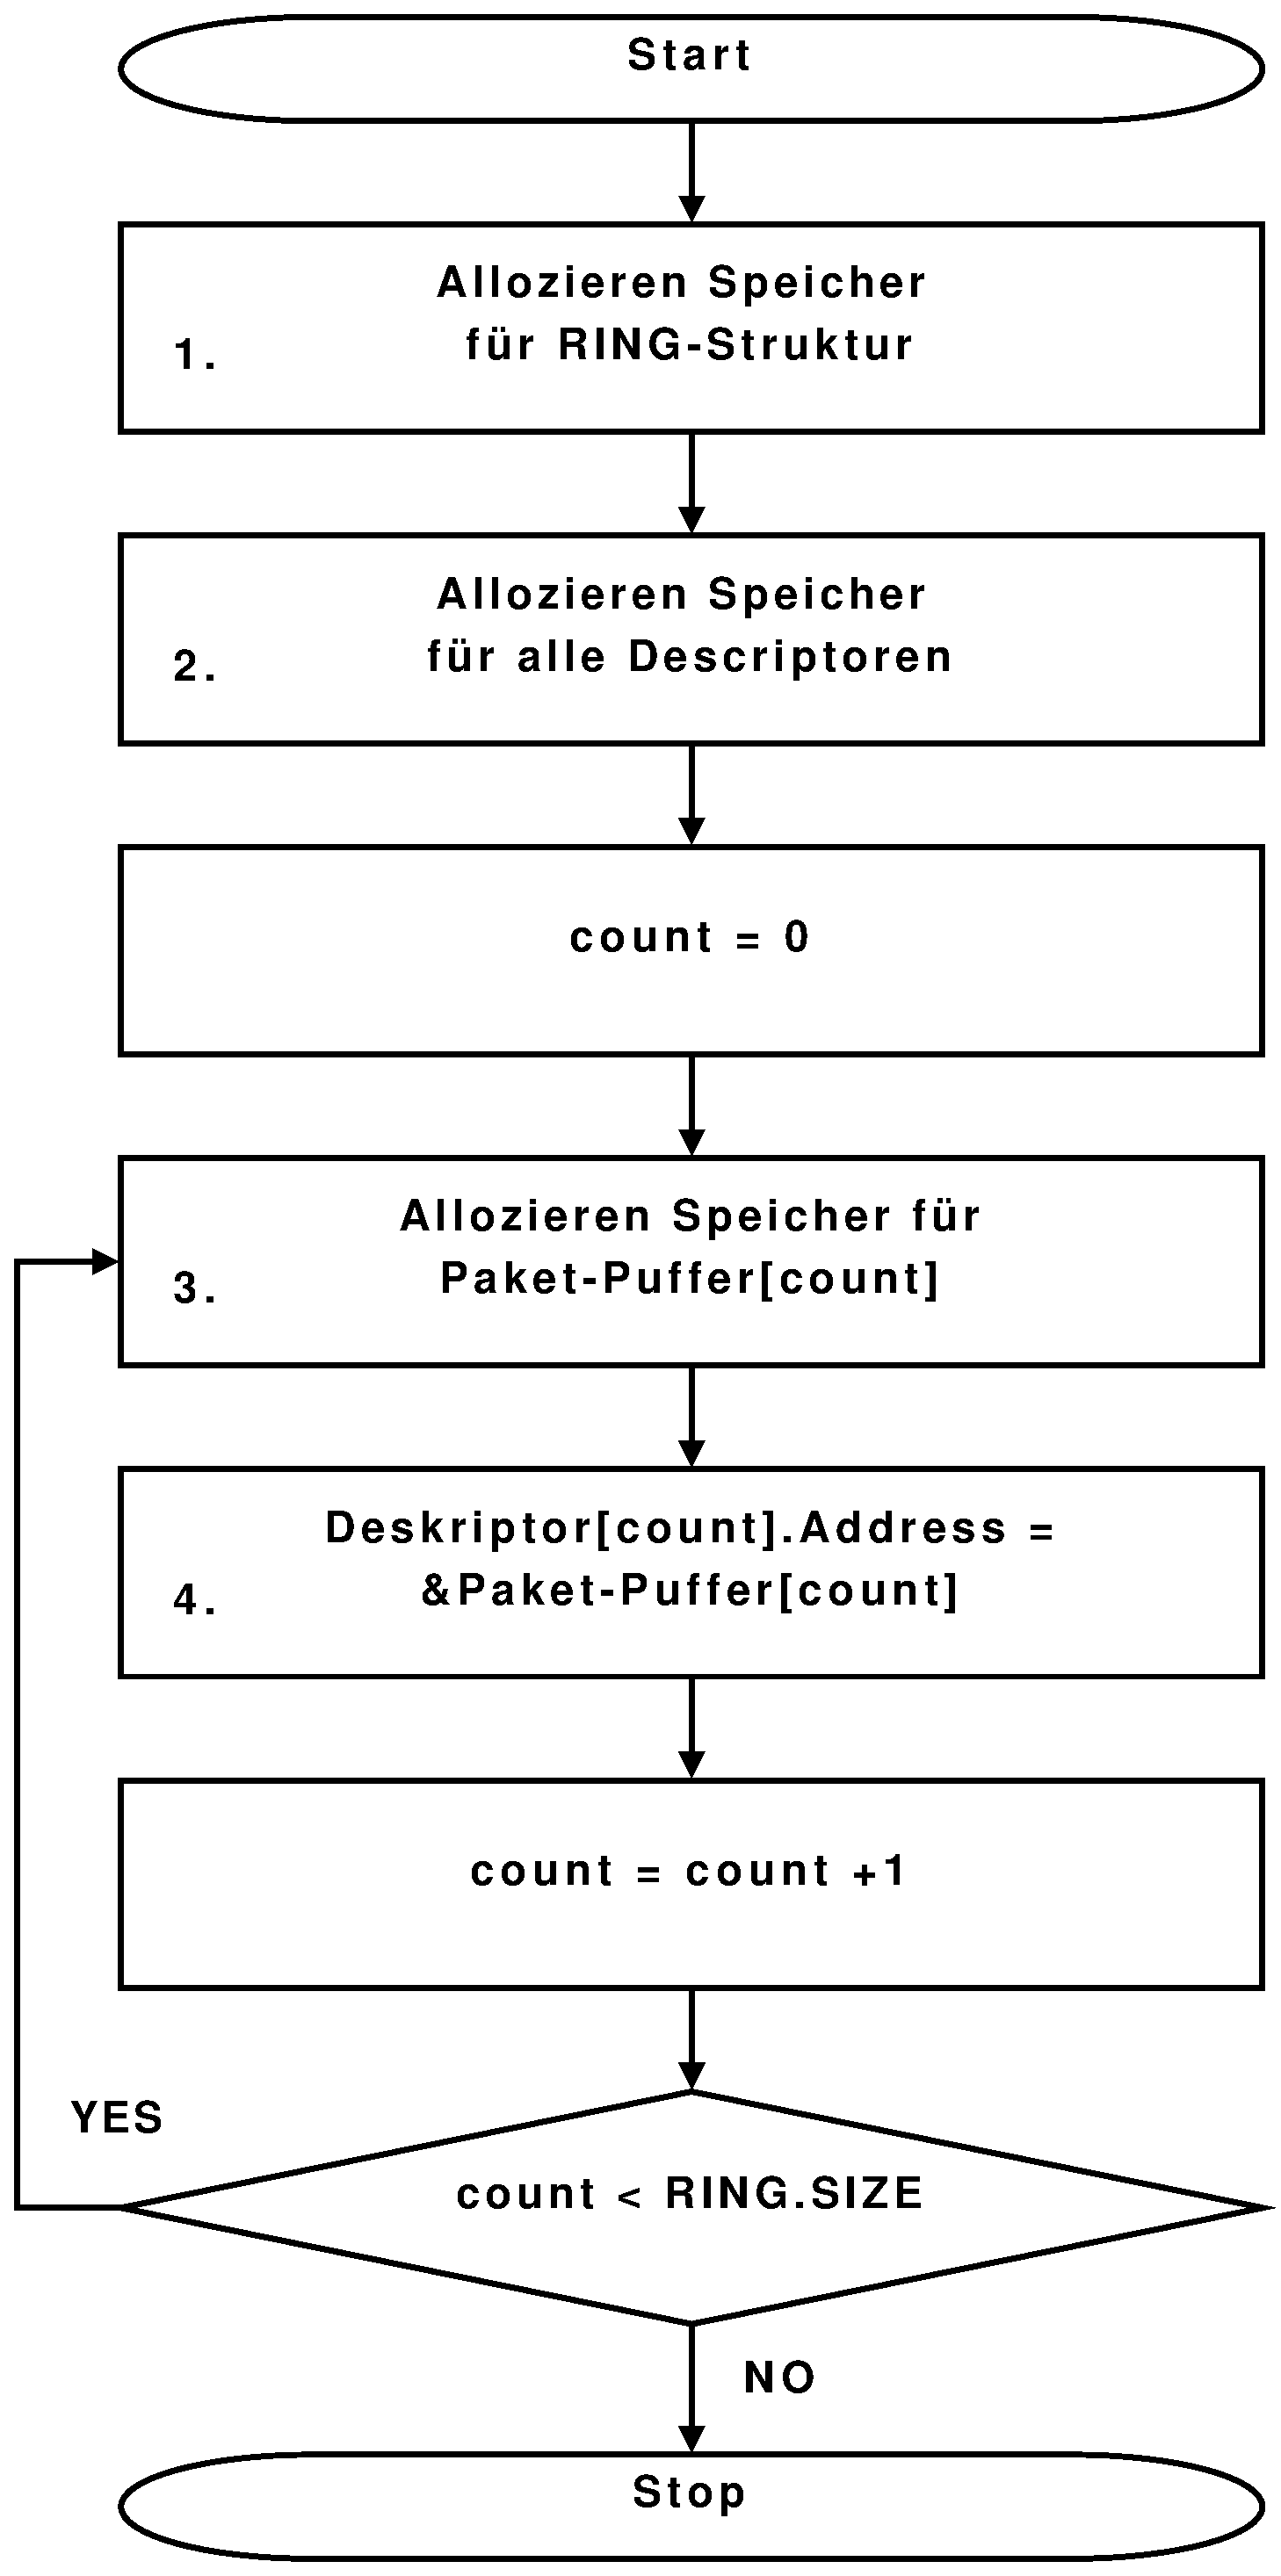
\includegraphics[width=3.9in]{bilder/FlowChart_Treiber_Init}
\caption{Treiber: Initialisierung}
\label{img:new_treiber_init}
\end{figure}
Die Initialisierungsfunktionen von Treiber werden beim Laden des Treibers
ausgeführt.  In Abbildung \ref{img:new_treiber_init} ist der Flow-Chart-Diagram
des Initialisierung-Prozesses dargestellt. Folgend beschreiben wir den den auf
dem Diagram dargestellten Algorithmus.
\begin{enumerate}
	\item Es wird den Speicher für \verb+RING+-Struktur alloziert.
	\item Der Speicher für alle Deskriptoren wird alloziert. Die physische
		Adresse des ersten Elementes von Deskriptor-Array wird in ein Register
		des Netzwerkadapters gesetzt, um dem Netzwerkadapter den Zugriff auf
		Deskriptoren zu ermöglichen~\cite{e1000_sdm}.
	\item Der Speicher für Paket-Puffer wird alloziert.
	\item Die physische Adresse des allozierten Paket-Puffer wird in den 
		\verb+Address+-Feld des Deskriptors geschrieben (siehe Abbildung
		\ref{dma-e1000-desc}). 
	\item Wiederhole die Schritte \textbf{3.} und \textbf{4.} für alle 
		\verb+RING+-Slots (bzw. Deskriptoren).
\end{enumerate}
Nach der Initialisierung-Phase des Treibers sind die Deskriptoren
kontinuierlich  im physischen Speicher alloziert und initialisiert. Darüber
hinaus sind die Paket-Puffer alloziert und die physische Adressen von den
Paket-Puffer sind in den \verb+Address+-Felder der Deskriptoren gesetzt (siehe
Abbildung \ref{dma-e1000-desc}). Nach dem setzen der physischen Adresse des 
ersten Deskriptor in den \verb+RDBAL+- und \verb+RDBAH+-Adapter-Register, 
kann der Netzwerkadaptern mit dem Capturing anfangen.

\subsubsection*{Ablauf des Capturing}\label{sec:new_treiber_ablauf}
Die \emph{Flow-Chart}-Diagram des Kernel-Threads ist in Abbildung
\ref{img:new_kernel_thread} dargestellt. Der Kernel-Thread bearbeitet maximal
\verb+rx_processing_limit+ Slots und beginnt mit dem Slot, dessen Nummer in der globalen
\verb+current_SLOT+-Variable gespeichert ist. Die Variable \verb+current_SLOT+ 
wird nach der Bearbeitung jedes Ringslots inkrementiert, sodass sie 
der Nummer des nächsten Slot im Ringpuffer entspricht.\\\\
Folgend beschreiben wir den Algorithmus  des neuen Kernel-Threads: 
\begin{enumerate}
	\item Speichern des \verb+RING.TAIL+-Wertes in RDT-Register 
		\begin{itemize}
			\item Der Userspace-Process soll nach dem Zugriff auf Paket den Wert
				\verb+RING.TAIL+ so erhöhen, dass \verb+RING.TAIL+ der
				Nummer des zuletzt gelesenen Slots entspricht.
			\item Der Kernel-Thread setzt \verb+RING.TAIL+-Wert in 
				RDT-Register und übergibt damit dem  Netzwerkadapter die neue freie
				Deskriptoren für den DMA-Transfer der nächsten Pakete (siehe
				Abschnitt \ref{sec:hw_dma}). 
		\end{itemize}
	\item Berechnen der Verkehrsstatistiken. 
		\begin{itemize}
			\item \emph{Time-Stamp} wird berechnet und in \verb+SLOT+-Struktur gesetzt.
		\end{itemize}
	\item \verb+current_SLOT+ \emph{modulo} \verb+RING.SIZE+ inkrementieren.
		\begin{itemize}
			\item \verb+current_SLOT+ ist dann die Nummer des nächsten 
				für Bearbeitung stehenden Slot.
		\end{itemize}
	\item  Der wert von \verb+current_SLOT+ wird in \verb+RING.HEAD+ gesetzt. 
		\begin{itemize}
			\item Damit wird für den  Userspace-Prozess noch ein Slot zur Verfügung
				gestellt.  Die Slots von \verb-RING.TAIL + 1- bis zu dem Slot
				mit der Nummer \verb+RING.HEAD - 1+ enthalten die neue Pakete,
				welche der Userspace-Prozess noch bearbeiten soll (siehe
				Abschnitt \ref{sec:hw_dma}). 
		\end{itemize}
	\item \verb+count+ wird dekrementiert.
	\item Der wartende Userspace-Capturing-Prozess wird ausblockiert wenn 
		der Kernel-Thread alle \verb+rx_processing_limit+ Paket-Puffer
		oder alle neue nach dem letzten Interrupt im RAM befindlichen Paket-Puffer 
		bearbeitet hat.
\end{enumerate}
%
\begin{figure}
\centering 
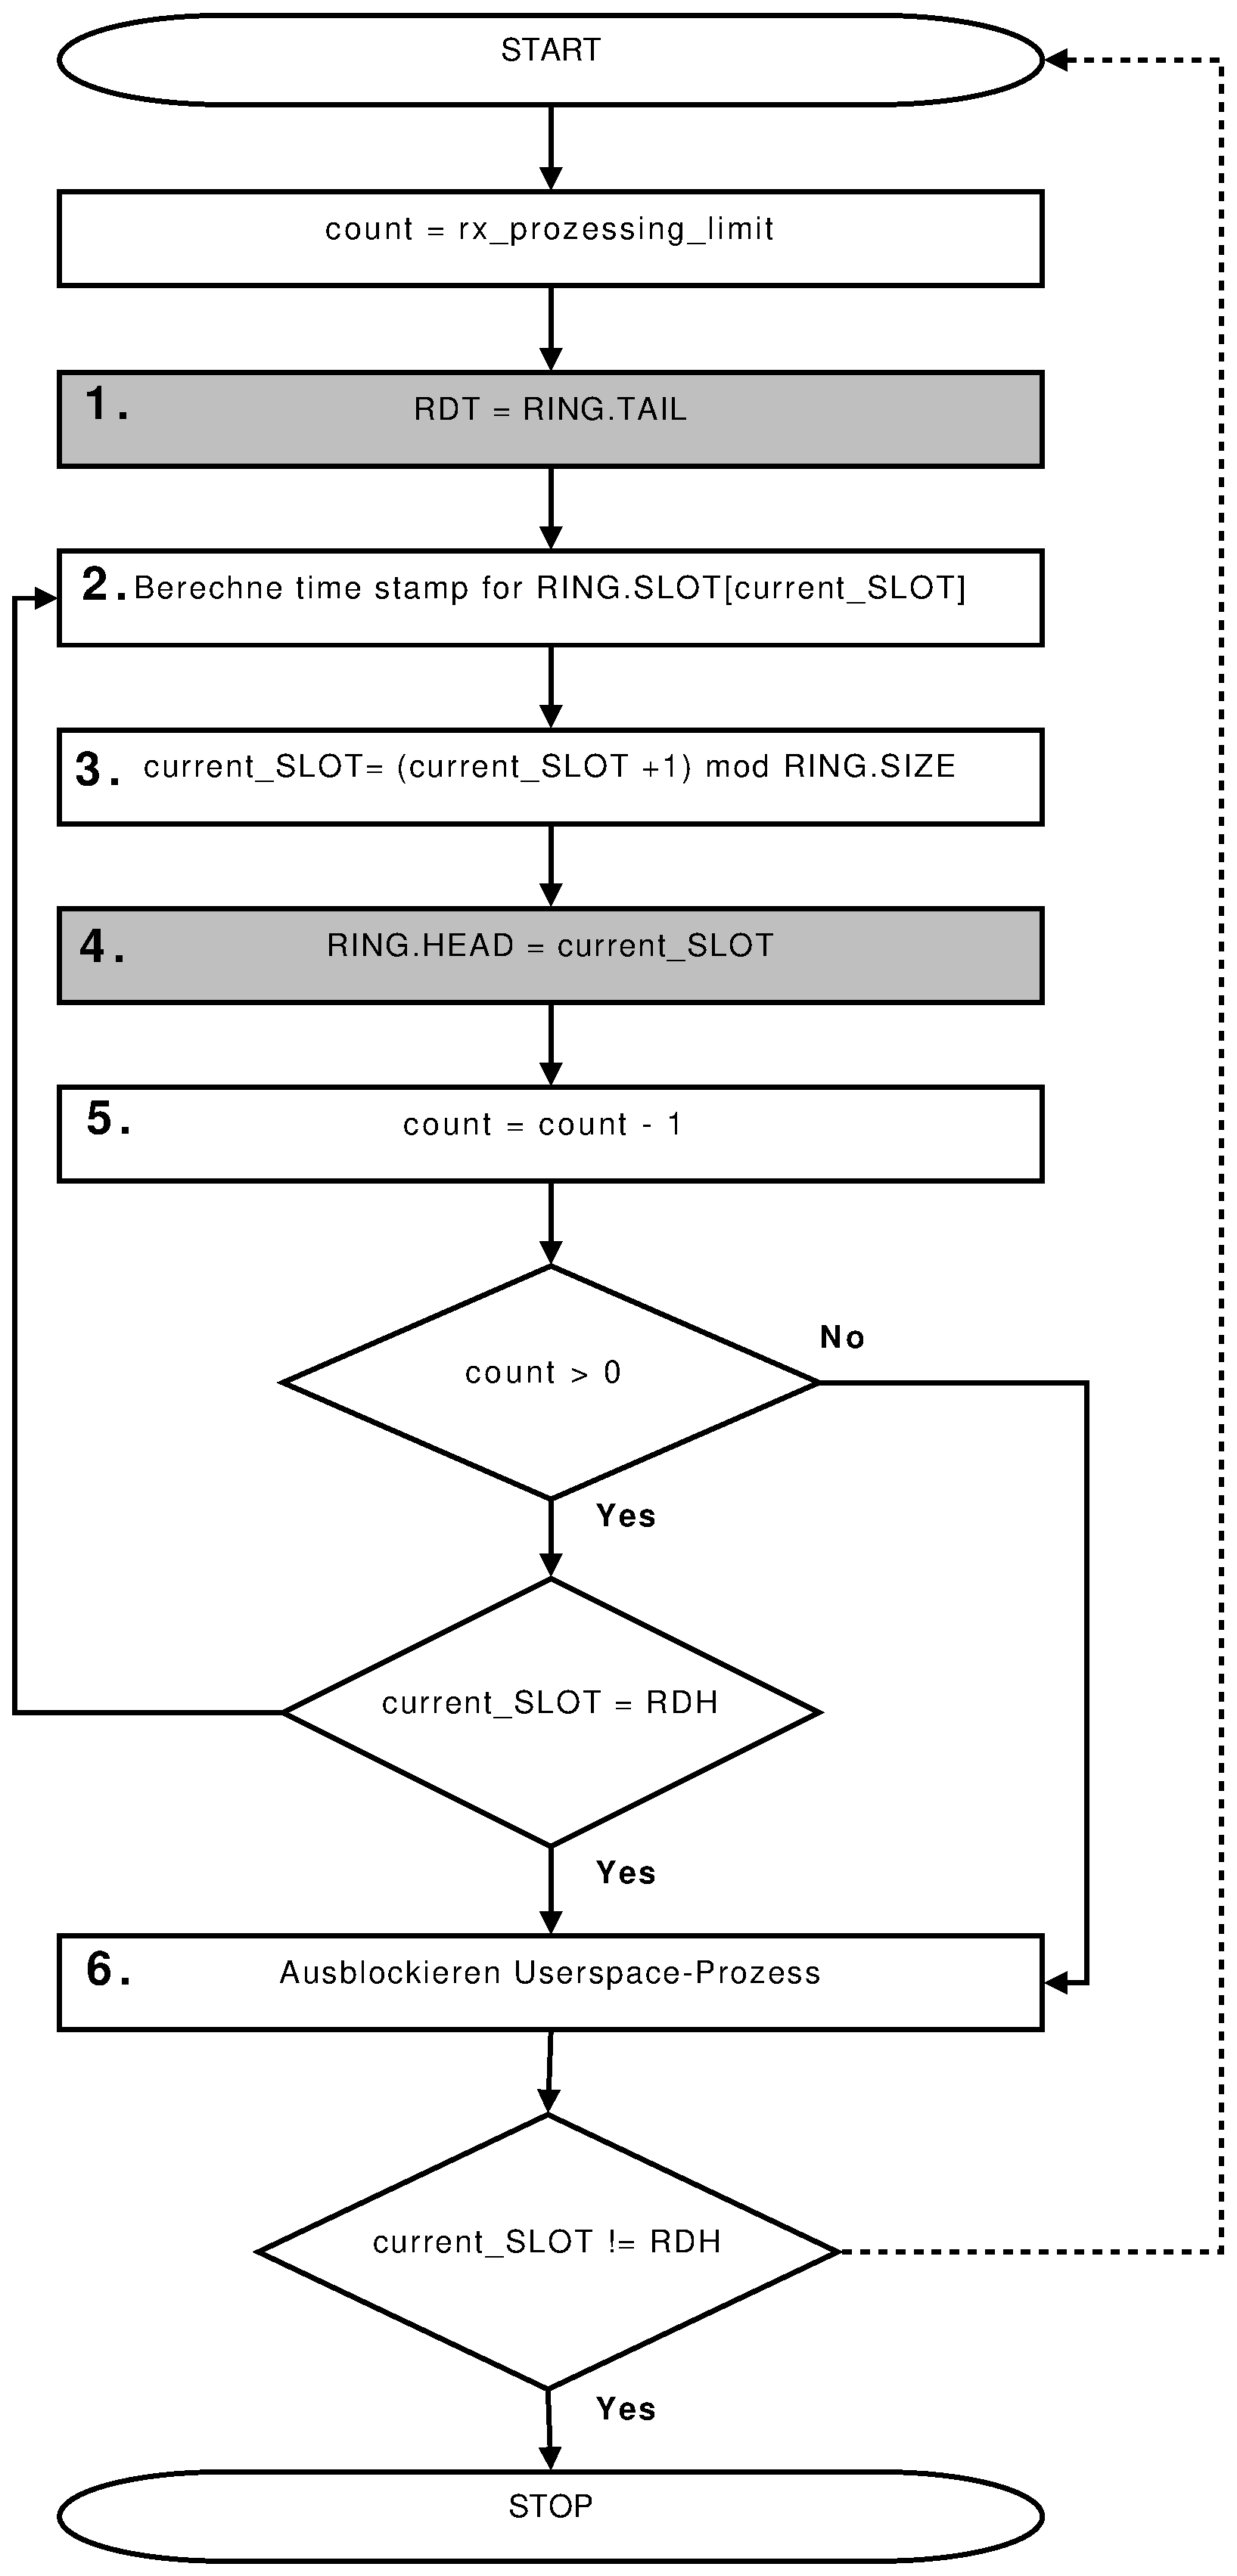
\includegraphics[width=4.2in]{bilder/FlowChart_New_Kernel_Thread}
\caption{Capturing-Ablauf. Kernel-Thread des \emph{ringmap}-Netzwerkadapter-Treibers}
\label{img:new_kernel_thread}
\end{figure}
Die graugezeichneten Boxen in Abbildung \ref{img:new_kernel_thread} bezeichnen
die Operationen, die zur Verwaltung von den \verb+TAIL+- und
\verb+HEAD+-Ringpointers dienen.  Dadurch, dass die \verb+RING+-Struktur in den
Userspace eingeblendet ist und damit sowohl im Userspace als auch im
Kernelspace zur Verfügung steht, können der Treiber und der Userspace-Prozess
durch das Setzen von \verb+RING.TAIL+- und \verb+RING.HEAD+-Pointers einander über
die gemachte Arbeit benachrichtigen. \\\\
%
Der Userspace-Prozess liest die neue
Paket-Puffer bis zu dem Paket-Puffer mit der Nummer \verb+RING.HEAD - 1+, und
wird blockiert für das Warten auf neue Pakete. Nach jeder Bearbeiten des neuen
Paket-Puffer setzt der Userspace-Prozess in \verb+RING.TAIL+ die Nummer der
gerade gelesenen Slot, und sobald der Kernel-Thread an der Reihe ist, liest der
Kernal-Tread diesen Wert und setzt ihn in  RDT-Register.\\\\
%
Der Netzwerkadapter-Treiber beschreibt die Paket-Puffer mit den neuen Daten beginnend
von dem Slot, desser Nummer im \verb+RDH+-Register bis zu dem Slot desser
Nummer im \verb+RDT+-Register gespeichert ist, und damit überschreibt nicht die
Paket-Puffer die von dem Userspace-Prozess noch nicht bearbeitet wurden.

\subsubsection{Systemaufruf-Funktionen}\label{sec:entw_syscalls}
Die Systemaufrufe sind dazu gebraucht werden, um dem Interaktion zwischen den
Netzwerkadapter-Treiber und Userspace-Capturing-Prozess zu ermöglichen. Dabei werden
dem Userspace-Prozess die Funktionen zur Verfügung zu gestellt, die er aufgrund
der Hardwarebegrenzungen nicht selber ausführen kann.\\\\ 
%
Die Systemaufrufe werden in unserem \emph{ringmap}-Capturing-Stack für die folgende
Zwecke gebraucht: 
\begin{itemize}
	\item Capturing-Steuerung
		\begin{itemize}
			\item Anhalten und Fortsetzen des Paketempfangs beim Netzwerkadapter
		\end{itemize}
	\item Memory-Mapping
		\begin{itemize}
			\item Allozieren und Initialisieren der \verb+RING+-Struktur (siehe
				Abbildung \ref{img:uml_ring}).
			\item Liefern dem Userspace-Prozess der physischen Adresse der
				\verb+RING+-Struktur.
			\item Das eigentliche \emph{Memory-Mapping} wird vom
				Userspace-Prozess durch den \emph{mmap}-Systemaufruf auf dem
				device \verb+/dev/mem+ realisiert.
		\end{itemize}
	\item Blockierendes Warten auf neue Pakete
		\begin{itemize}
			\item Sobald keine neue Pakete zur Bearbeitung für den
				Userspace-Prozess im RAM liegen wird der Userspace-Prozess
				blockiert und erst nach dem Ankommen der neuen Pakete
				durch den Kernel-Thread wieder ausblockiert (siehe Abschnitt
				\ref{sec:new_treiber_ablauf}, Abbildung
				\ref{img:new_kernel_thread})
		\end{itemize}
\end{itemize}
\subsubsection*{Capturing-Steuerung}
Capturing-Steuerung wird mit Hilfe des \emph{ioctl}-Systemaufrufes realisiert.
Die primäre Aufgaben dabei sind \emph{Capturing-Anhalten} und
\emph{Capturing-Fortsetzen}.  Die Idee liegt daran, dass der Userspace-Prozess
einen \emph{ioctl}-Systemaufruf macht, dann wird die für den Aufruf
verantwortliche Funktion im Kernelspace ausgeführt, welche über die Beschreiben
des Control-Register des Netzwerkadapters den Paketempfang anhält oder
fortsetzt.\\\\ 
%
Die Details sind im Kapitel \textbf{Implementierung} im Abschnitt
\ref{sec:impl_treiber} beschrieben.
 
\subsubsection*{Memory-Mapping}\label{sec:memmap}
Die Memory-Mapping wird mit dem \emph{mmap}-Systemaufruf auf dem Device
\verb+/dev/mem+ realisiert. Als Argument bekommt der \emph{mmap} die physische
Adresse und die Byte-Länge des Speicherbereiches, der in den Userspace
eingeblendet wird, und liefert dem Userspace-Prozess die gültige
Userspace-Adresse des eingeblendeten Speicher-Bereich zurück.\\\\
%
Das heißt, der Userspace-Capturing-Prozess soll für das Einblenden der
Paket-Puffer und \verb+RING+-Struktur  erstmal im Besitz der physischen
Adressen zu sein. Diese können aufgrund der funktionalen User-Mode-Begrenzungen
nur im Kernelspace bekommen werden. Das hat zur Folge, dass es außer
\emph{mmap} noch ein Systemaufruf zum Bekommen der physischen Adressen
gebraucht wird. \\\\
%
Die Aufgaben der für diesen Systemaufruf im Kernelspace verantwortlichen
Funktion sind folgende: 
\begin{itemize}
	\item Allozieren des Speicherbereiches für \verb+RING+-Struktur
	\item Initialisieren der \verb+RING+ mit den physischen Adressen 
		von den Paket-Puffern und Deskriptoren
	\item Die physische Adresse der \verb+RING+-Struktur zurückgeben
\end{itemize}
Sobald der Userspace-Prozess die physische Adresse der \verb+RING+-Struktur
hat, kann er \verb+RING+ in seinen Adressraum einblenden. Dann hat er auch die
physische Adresse der Paket-Puffer und Deskriptoren, weil diese im \verb+RING+
gespeichert wurden. Mit dem Kenntnis der physischen Adressen ist es dem 
Userspace-Prozess möglich die Paket-Puffer und die Deskriptoren in seinen 
Adressraum einzublenden und mit dem Capturing anfangen.

\subsubsection*{Blockierendes Warten auf neue Pakete}
Dem Userspace-Capturing-Prozess soll es möglich sein, während des Warten auf
neue Pakete blockiert zu werden. Ohne Kernel-Unterstützung wäre es nicht
möglich, denn nur Kernel des Betriebssystem in der Lage ist die
Prozesse zu blockieren.  Deshalb, soll dem Userspace-Prozess einen Systemaufruf
zur Verfügung gestellt werden, der ihm sich zu blockieren erlaubt hätte. \\\\
%
Im FreeBSD gibt es schon dafür einen Systemaufruf \emph{nanosleep(2)}. Dieses 
Systemaufruf erlaubt nur einen Prozess für eine bestimmte Zeit zu blockieren. 
Wir wollen aber etwas mehr und deshalb wurde für unsere Zwecke einen 
neuen Systemaufruf implementiert. \\\\
%
Die Aufgaben der für diesen Systemaufruf im Kernelspace verantwortlichen
Funktion sind folgende: 
\begin{itemize}
	\item Die für Capturing relevante Statistiken zu aktualisieren
	\item Den Wert von \verb+RING.TAIL+ in \verb+RDT+-Register
		setzen. Damit bekommt der Netzwerkadapter neue Deskriptoren für 
		den Transfer in den RAM neu angekommenen Pakete.
	\item Den Prozess für bis zu dem Auftreten des nächsten Interrupts 
		``im Schlaf'' legen, und dabei für diesen Prozess die höchste
		Priorität zu setzen.
\end{itemize}
Unser Systemaufruf erlaubt uns während Warten auf neue Pakete die für Capturing
relevante Statistiken zu aktualisieren, ohne dabei auf dem Interrupt zu warten.
Außerdem wird den Inhalt der \verb+RDT+-Registers aktualisiert, was dem Netzwerkadapter
die Zusätzliche Deskriptoren zur Verfügung stellt.  Und was sehr wichtig ist,
bekommt der schlafende Prozess die höhste Priorität, was dazu führt, dass, nach
dem Interrupt, beim Umschalten des System in User-Mode wird der Prozess als
einer der ersten wartenden Prozessen aufgewacht und damit mit der kleinste
Verzögerung mit der Bearbeitung der neuen Pakete anfängt. Dies kann sehr
wichtig im Fall der hohe Verkehrsrate sein, denn in dieser Situation wird vom
Userspace-Capturing-Prozess unverzügliche Bearbeitung der Pakete und damit die
möglichst schnelle Befreiung der benutzten Deskriptoren erwartet.
 
\subsubsection{Userspace-Anwendung}
Paketzugriff-Prozess wird im Userspace ausgeführt.  Die Aufgabe des
Userspace-Capturing-Prozesses ist es, die Pakete in den eingeblendeten
Paket-Puffer zu zugreifen mit dem Ziel diese  zu bearbeiten und eventuell zu
speichern.  Um den Zugriff auf die Pakete zu bekommen, soll der
Userspace-Prozess zuerst die Einblendung der der Paket-Puffer in seinen
Adressraum zu initiieren.  Dies wird in der Initialisierungsphase des
Prozesses geschehen.\\\\
%
Wenn die Paket-Puffer in Userspace eingeblendet sind, kann es mit dem Capturing
angefangen werden. Der User-Prozess liest bzw. bearbeitet alle Paket-Puffer
(\emph{Ring-Slots}) die Reihe nach, und wenn keine neue Pakete im RAM vorhanden
sind, wird er solange blockiert bis die neue Pakete ankommen.

\subsubsection*{User-Capturing-Prozess. Initialisierung}
In Abbildung \ref{img:us_init} ist das Algorithmus der Initialisierungsphase
des User-Prozess dargestellt. Bevor der User-Prozess den Zugriff auf die Pakete
bekommt, soll er die Initialisierung und die Einblendung der 
\verb+RING+-Struktur in sein Adressraum initiieren.  Dafür wird die physische
Adresse des \verb+RING+-Struktur gebraucht. \\\\
%
Um die \verb+RING+-Struktur zu initialisieren und die physische Adresse von ihr
zu bekommen wurde extra Funktionalität entworfen (siehe Abschnitt
\ref{sec:memmap}). Um diese Funktionalität zu benutzen soll der
Paketzugriff-Prozess einen Systemaufruf machen, der entsprechende Funktion im
Kernelspace ausführt.  Im Userspace wird dieser Systemaufruf mit der
\emph{read()}-Funktion mit Eingabe  des symbolischen Devise des Treibers
gemacht (siehe Kapitel \ref{sec:impl_treiber}).\\\\
%
Das Ausführen des Systemaufrufes verursacht das Allozieren der
\verb+RING+-Struktur, Initialisierung der \verb+RING+ mit den physischen
Adressen der Paket-Puffer und Rückgabe der physischen Adresse der
\verb+RING+-Struktur. Mit dem Kenntnis der physischen Adresse macht der
Userspace-Capturing-Prozess durch \emph{mmap}-Systemaufruf die Einblendung der
\verb+RING+-Struktur in seinen virtuellen Speicherraum. Dann hat er den Zugriff
physische Adressen der Paket-Puffer und blendet diese dann auch auf
gleicherweise seinen Speicherraum ein.\\\\
Sobald der Capturing-Prozess den Zugriff auf Paket-Puffer hat, kann er mit dem 
Capturing anfangen.

\begin{figure}
\centering 
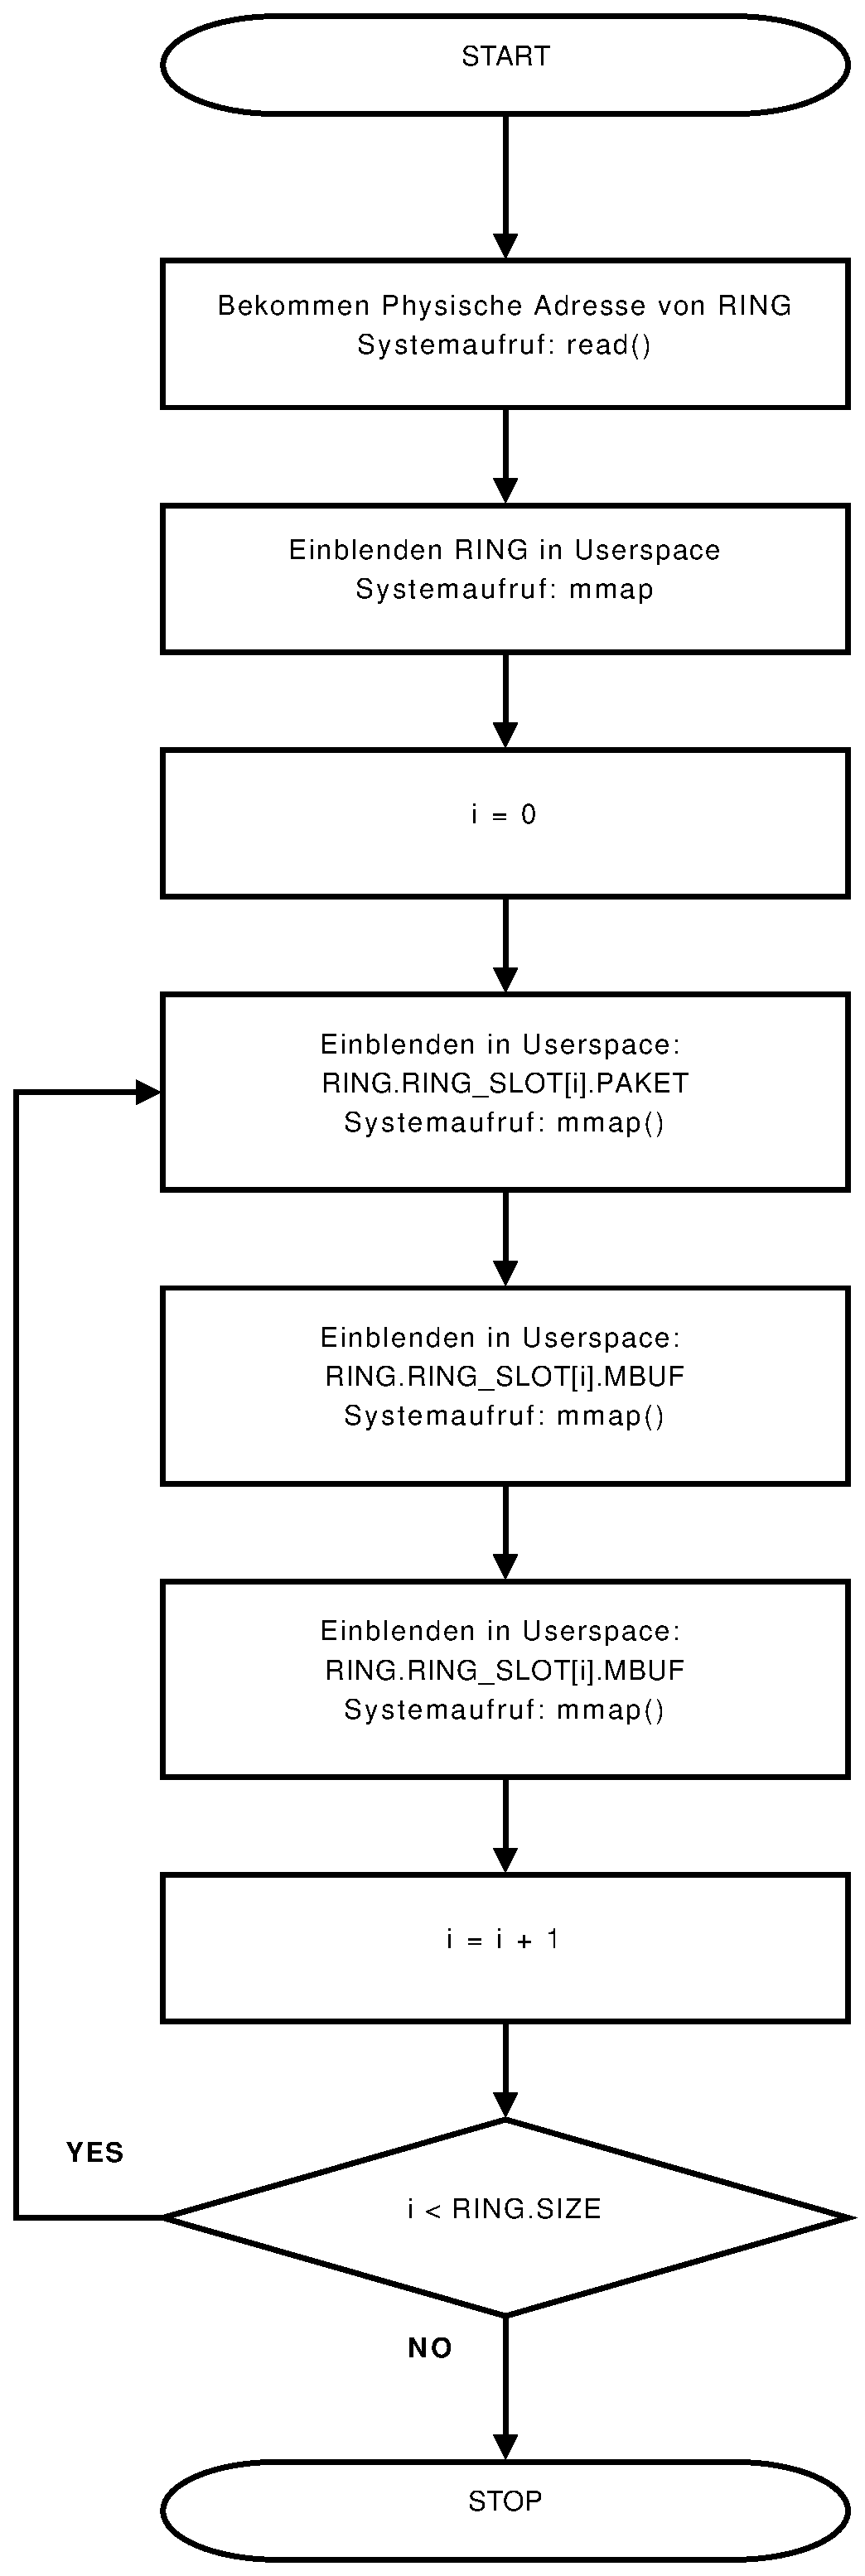
\includegraphics[width=3.0in]{bilder/FlowChart_US_Init}
\caption{User-Prozess. Initialisierung}
\label{img:us_init}
\end{figure}
 
\subsubsection*{User-Capturing-Prozess. Capturing}
\begin{figure}
\centering 
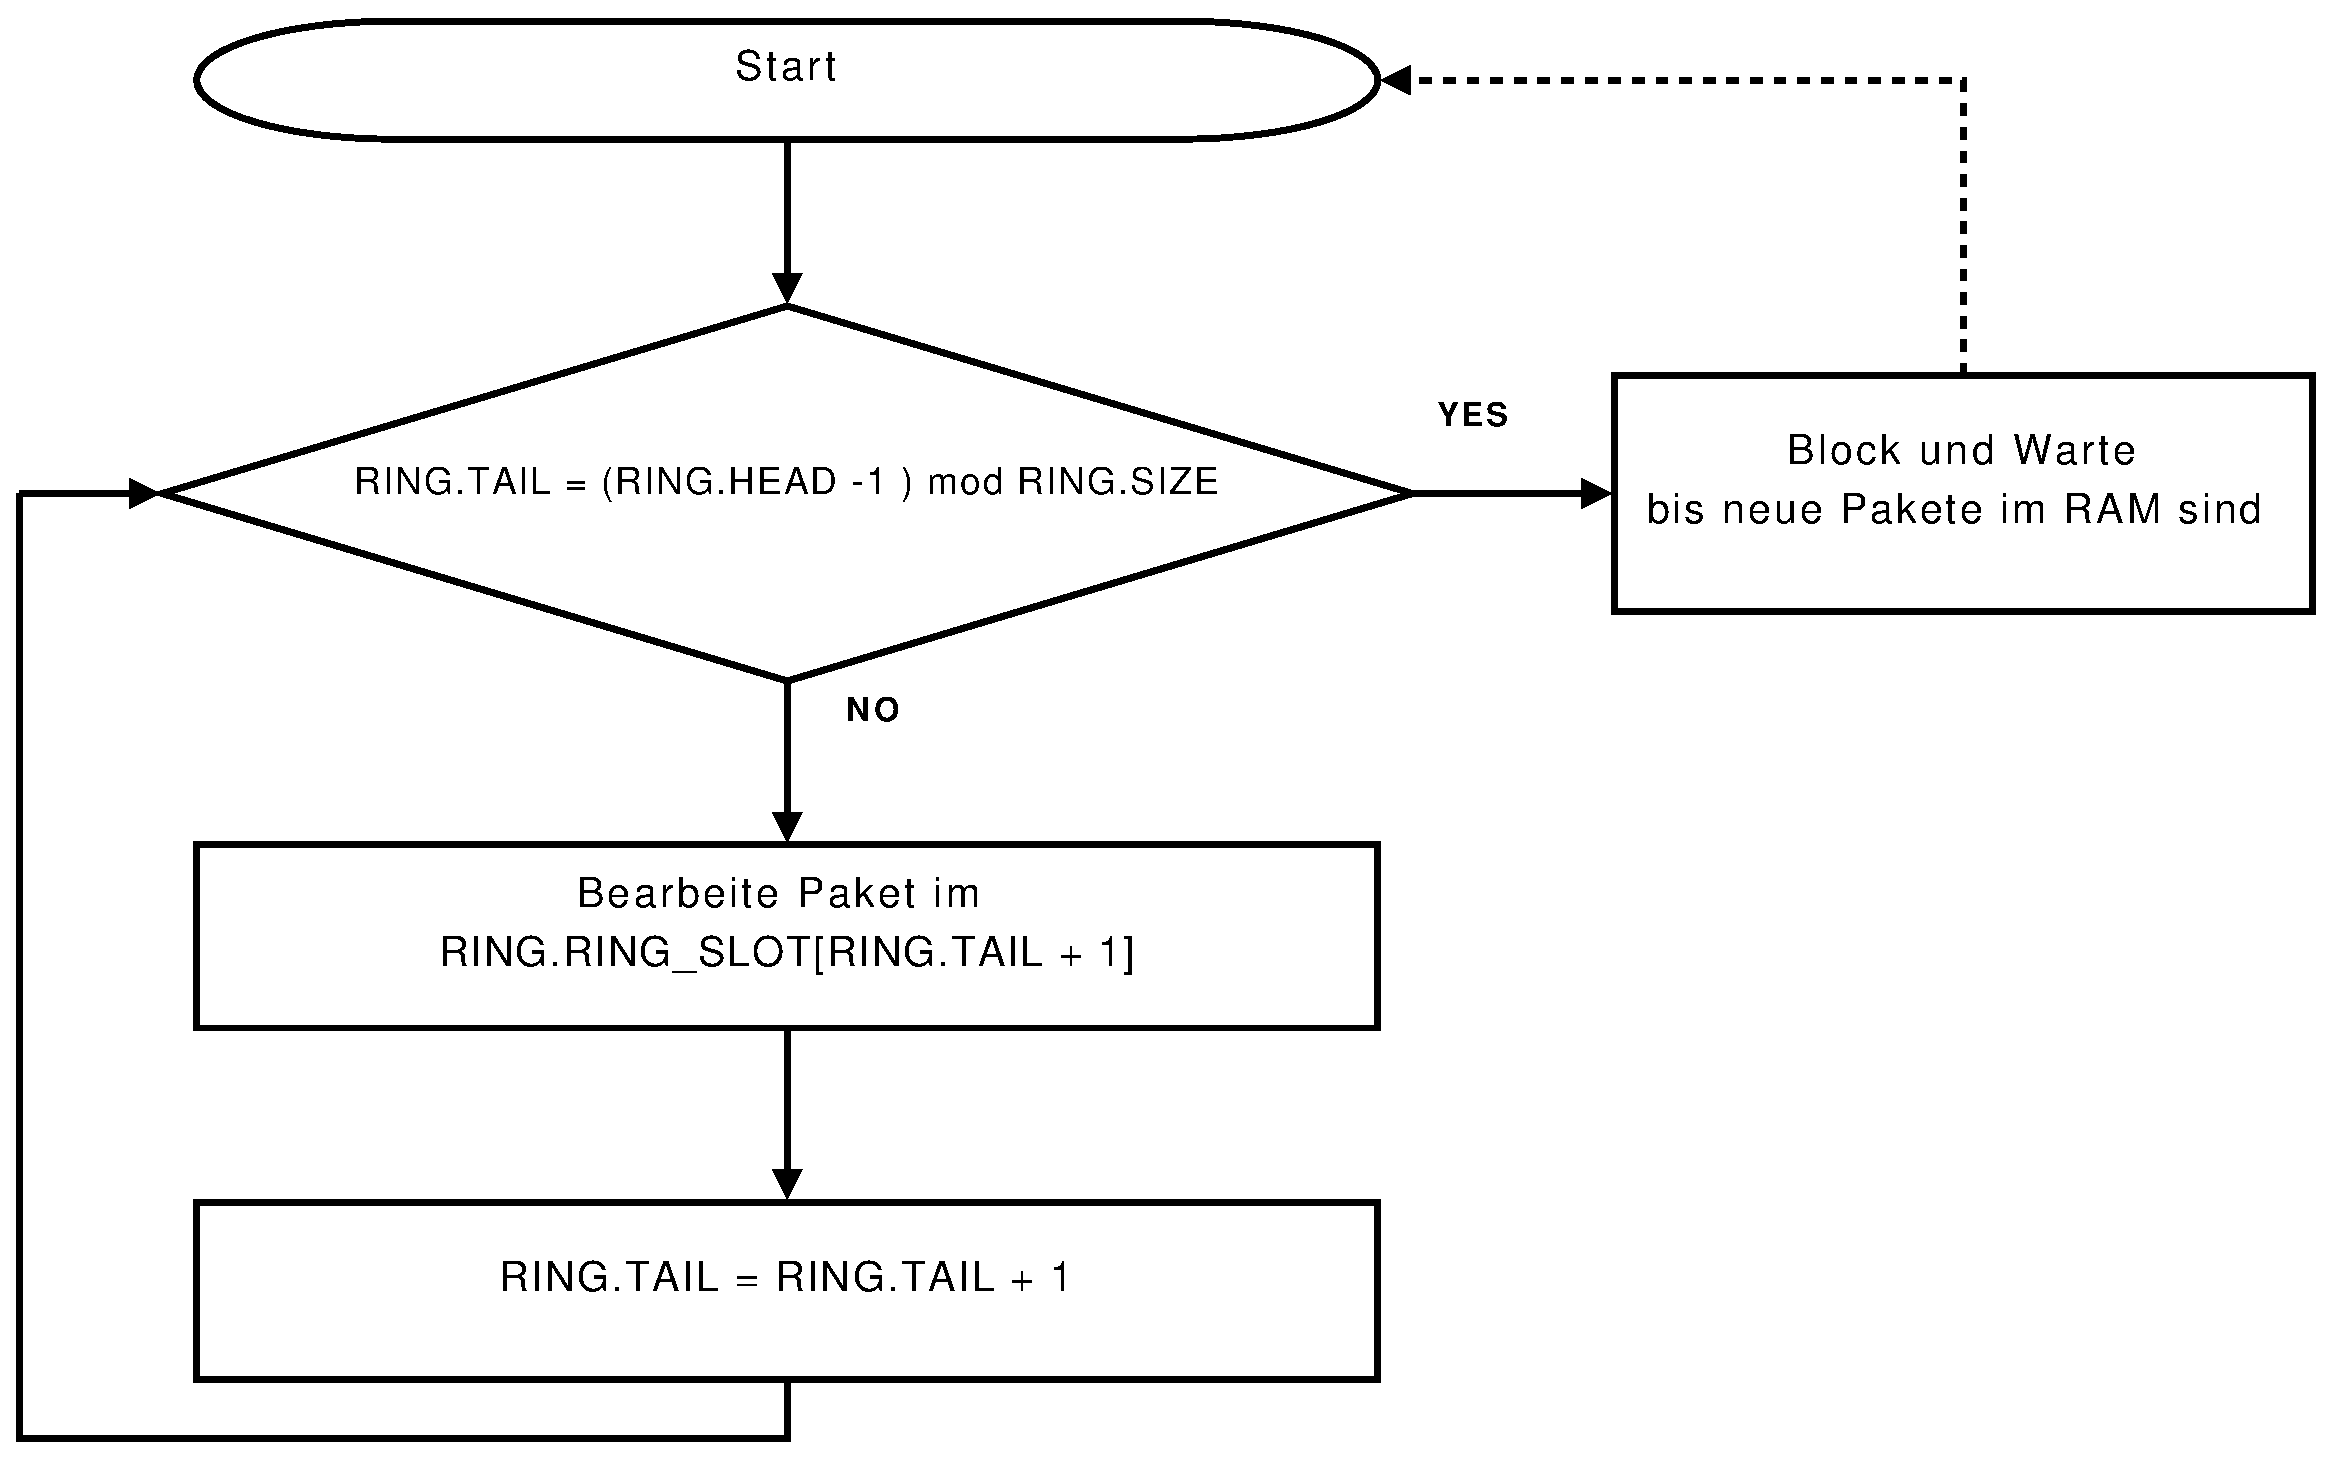
\includegraphics[width=6.0in]{bilder/FlowChart_US_CAP}
\caption{User-Prozess. Capturing-Ablauf}
\label{img:us_capt}
\end{figure}
In Abbildung \ref{img:us_capt} ist der Ablauf des Capturing
in Userspace dargestellt. Der Userspace-Capturing-Prozess liest die \verb+RING_SLOT+'s in der \verb+RING+-Struktur 
der Reihe nach. Nimmt aus den Slots die benötigte Adresse der Paket-Puffer, \verb+mbuf+'s, 
Deskriptoren, und danach bearbeitet bzw. filtert die Pakete, die in den Paket-Puffer
enthalten sind. Beim Bearbeiten jedes Paketes beschreibt der Capturing-Prozess
den \verb+RING.TAIL+ mit der Nummer des gerade gelesenen Paket-Puffer. Sobald 
der \verb+RING.TAIL+ den \verb+RING.HEAD+ nachgeholt hat, was die Abwesenheit 
von neuen Paketen im RAM bedeutet, wird der Prozess blockiert. Sobald die 
neue Pakete in den RAM ankommen, wird nach der Interruptbehandlung der Prozess 
wieder erweckt. \\\\
%
Dadurch, dass der Userspace-Capturing-Prozess sowohl die Paket-Puffer als auch
die \verb+mbuf+'s und Deskriptoren in seinem virtuellen Speicher hat, kann er
aufwendige Paket-Bearbeitung machen. Über die Deskriptor-Felder ist jetzt dem
Userspace-Prozess unterschiedliche Details, die der Netzwerkadapter zur Verfügung
stellt (\verb+Checksum, Lenght, Error+, etc\ldots ) bekannt. Das heißt, man braucht 
keine CPU-Lästige Systemaufrufe um den Zugriff auf die Informationen zu bekommen.

\subsection{Zusammenfassung}
In diesem Kapitel wurde den Entwurf des neuen ringmap-Paket-Capturing-Stack
vorgestellt.  Die Funktionen des Stacks sind für \emph{Paketzustellung},
\emph{Paketzugriff} und \emph{Capturing-Steuerung} zuständig. Die Zustellung-
und Zugriff-Prozess benutzen gemeinsam mehrere Speicher-Bereiche
(\emph{shared-Memory}), die mit Hilfe der \verb+RING+-Struktur in Form eines
Ringpuffers modelliert sind.  Die \verb+RING+-Struktur und  die für
Paketempfang verantwortliche Paket-Puffer sind in Adressraum sowohl des
Zustellung-Prozesses als auch des Zugriff-Prozesses eingeblendet. Dies
ermöglicht den Paketzugriff ohne das teure Kopieren und ohne Systemaufrufe.\\\\
%
Der Zustellung-Prozess wird im Kernelspace und der Zugriff-Prozess im Userspace
ausgeführt. Aufgrund dass es nur einen Zustellung-Prozess und nur einen
Zugriff-Prozess gibt entstehen keine \emph{race conditions}. Deshalb werden
Synchronisation-Massnahmen benötigt.\\\\
%
Für den Zugriffsprozess ist die Funktionalität entworfen, die es ihm erlaubt im
blockierten Zustand auf die neue Pakete zu warten, das Capturing anzuhalten und
wieder fortzusetzen und die Einblendung der für Paketempfang verantwortlichen
Speicherbereichen zu initiieren. Diese Funktionalität soll im Kernelspace
ausführbar sein und dadurch über die Systemaufrufe zur Verfügung stehen.\\\\
Die Implementierungsdetails des Entwurfes sind im folgenden Kapitel
dargestellt.

\newpage
\ifthenelse{\boolean{BRIEF}}{}{ 
\section{Implementierung}
\lstset{language=C}
Das in diesem Kapitel vorgestellten Material wird die Implementierungs-Details
des neuen \emph{ringmap}-Paket-Capturing-Stack darstellen. Die vorgestellten hier Code-Abschnitte
haben keine exakte übereinstimmung mit dem implementierten Code: es sind nur
die wichtigste Details dargestellt, die sich im Zusamenhang mit den im Kapitel
\textbf{Entwurf} vorgestellten Algorithmen stehen. Für das eingehende
Verständnis des Codes gibt es ausführliche Kommentare im Code.

\subsection{Datenstrukturen}
Die in diesem Kapitel dargestellten Datenstrukturen sin in der \verb+fiveg_da.h+ Datei deklariert. 
\subsubsection{Ringpuffer}
\subsubsection*{RING}
\begin{lstlisting}[frame=single, caption={RING-Struktur}, captionpos={b}, label={code:ring_struct}]
struct ring {
	unsigned int kernrp;
	unsigned int userrp;
	unsigned int size;
	struct ring_slot slot[SLOTS_NUMBER];
};
\end{lstlisting}
\begin{itemize}
	\item \textbf{kernrp}: \verb+RING.HEAD+ - HEAD-Pointer. Soll nur im Kernelspace geändert werden. 
	\item \textbf{userrp}: \verb+RING.TAIL+ - TAIL-Pointer. Soll nur im Userspace geändert werden.
	\item \textbf{size}: \verb+RING.SIZE+ - Anzahl der Slots im Ringpuffer.
	\item \textbf{slot}: \verb+RING.RING_SLOT+-Array - Array von Slots. 
\end{itemize}
\subsubsection*{RING\_SLOT}
\begin{lstlisting}[frame=single, caption={RING-SLOT-Struktur}, captionpos={b}, label={code:ring_slot_struct}]
struct ring_slot {
	struct address 	descriptor;
	struct address 	mbuf;
	struct address	packet;
	struct timeval	ts;
	unsigned long long cnt;
};
\end{lstlisting}
\begin{itemize}
	\item \textbf{descriptor}: \verb+DESKRIPTOR+ - Für Adressierung der Deskriptoren
	\item \textbf{mbuf}: \verb+MBUF+ - Für Adressieren der \verb+mbuf+'s
	\item \textbf{packet}: \verb+PAKET+ -  Für Adressieren des Paket-Puffers
	\item \textbf{ts}: \verb+TIME_STAMP+ - Paket-Timestamp. Wird beim Treiber berechnet.
	\item \textbf{cnt}: \verb+SLOT_COUNTER+ - Paket-Counter
\end{itemize}
\subsubsection*{ADDRESS}
\begin{lstlisting}[frame=single, caption={ADDRESS-Struktur}, captionpos={b}, label={code:address_struct}]
struct address {
	bus_addr_t 	phys;
	vm_offset_t	kern;
	vm_offset_t	user;
};
\end{lstlisting}
\begin{itemize}
	\item \textbf{phys}: \verb+PHYS_ADDR+ - Physische Adresse des adressierten Elementen
	\item \textbf{kern}: \verb+KERN_ADDR+ - Kernelspace-Adresse des adressierten Elementen
	\item \textbf{user}: \verb+USER_ADDR+ - Userspace-Adresse des adressierten Elementen
\end{itemize}
\subsection{Funktionalität}
Die für den \emph{ringmap}-Paket-Capturing-Stack implementierten Funktionalitäten
betreffen sich \emph{Netzwerkadapter-Treiber}, \emph{Libpcap}-Library und
Kernel-Funktionen, die in Folge der \emph{Systemaufrufen} ausgeführt werden.\\\\
Alle Änderungen in der generischen Dateien des \textbf{em}-Treiber und Libpcap
sind in über Makrodefinition \verb+__FIVEG_DA__+ eingetragen. Zum Beispiel:
\begin{lstlisting}[frame=single, caption={Code-Einträge in Dateien des generischen em-Treiber}, captionpos={b}, label={code:code_eintr}]
	. . . 
#ifdef __FIVEG_DA__
	adapter->rm->ring.interrupts_counter++;
	/* Make interrupt time stamp in the adapter structure */
	getmicrotime(&adapter->intr_ts);
#endif
	. . . 
\end{lstlisting}	
\subsubsection{Treiber. Paketzustellung}\label{sec:impl_treiber}
Für den \emph{ringmap}-Treiber wurde als Basis der generische \textbf{em}-Treiber
genommen.  In den Funktionen des generischen \textbf{em}-Treibers wurden kleine
Änderungen gemacht und dazu noch die neue Funktionen implementiert, die den
Treiber der im Abschnitt \ref{sec:aufgstel} gestellten Anforderungen
entsprechend machen.\\\\ 
%
Die für den \emph{ringmap}-Treiber implementierten Funktionalitäten befinden sich zum
grossen Teil in der Datei \verb+fiveg_da.c+. In den generischen Dateien des
Treibers wurden nur kleine Änderungen gemacht, die meistens nur die
Funktionsaufrufe aus \verb+fiveg_da.c+ enthalten. \\\\
%
Die Funktionen des Treiber lassen sich in drei Kategorien Teilen: 
\begin{itemize}
	\item Initialisierung-Funktionen:
		\begin{itemize}
			\item werden beim Laden des Treibers aufgerufen.
		\end{itemize}
	\item Systemaufruf-Funktionen
		\begin{itemize}
			\item Kernel-Funktionen, die infolge eines Systemaufrufes aufgerufen werden.
		\end{itemize}
	\item Interruptsbehandlung-Funktionen
		\begin{itemize}
			\item \emph{Interrupt-Service-Routine} und Kernel-Thread, die infolge eines 
				Interrupt-Ereignisses aufgerufen werden und welche für Capturing-Ablauf
				zuständig sind.
		\end{itemize}
\end{itemize}

\subsubsection*{Initialisierung}
Während des Ladens des Treiber werden unter Anderem folgende Funktionen aufgerufen: 
\begin{itemize}
	\item \verb+em_probe()+: Datei \verb+if_em.c+. Ist für das Erkennen der
		Netzwerkadapter-Modelles verantwortlich. 
	\item \verb+em_attach()+: Datei \verb+if_em.c+. Diese Funktion ist für alle
		Initialisierung-Prozesse zuständig. Hier werden unter Anderem die
		Speicherbereiche für Deskriptoren und Paket-Puffer alloziert.
	\item \verb+ringmap_attach()+: Datei \verb+fiveg_da.c+. Wird aus der
		\verb+em_attach()+ aufgerufen. Alloziert den Speicher für
		\verb+ring+-Struktur und erzeugt ein neues symbolische Device
		\verb+/dev/ringmap+. Über dieses Device  wird der
		Userspace-Capturing-Prozess mit Hilfe der Systemaufrufen \verb+read+
		und \verb+ioctl+ \emph{Capturing-Steuerung}, \emph{Mempory-Mapping} und
		\emph{Blokierendes Warten} anfordern (siehe Abschnitt
		\ref{sec:entw_syscalls}).
\end{itemize}
Für das Kompilieren aller Software für den \emph{ringmap}-Capturing-Stack und Laden des Treibers 
wurde den Skript \verb+ringmap_build_and_load+ implementiert. Der Skript befindet sich 
im Verzeichnis \textbf{scripts/}\footnote{SVN-URL:
\url{https://svn.net.t-labs.tu-berlin.de/svn/alexandre-da/src/70/scripts/}}
im Code-Repository.

\subsubsection*{Treiber. Systemaufruf-Funktionen}
Um dem Userspace-Prozess die Interaktion mit dem Treiber und dadurch die
Capturing-Steuerung zu ermöglichen, registriert der Treiber bei der
\textbf{Initialisierung} das symbolische Device \verb+/dev/ringmap+ und bietet
eine Menge von Kernel-Funktionen an, die in folge der Systemaufrufen auf dem
device \verb+/dev/ringmap+ ausgeführt werden:
\begin{itemize}
	\item \verb+ringmap_open()+: wird in foge des \emph{open}-Systemaufrufes
		ausgeführt.  Checkt die für den Capturing benötigte Datenstrukturen.
		Prüft ob alle Speicher-Bereiche alloziert und zugreifbar sind.
	\item \verb+ringmap_read()+: Wird in folge des \emph{read}-Systemaufrufes
		ausgeführt.  Initialisiert die \verb+ring+-Struktur mit den physischen
		Adressen von den Paket-Puffer und Deskriptoren. Und liefert dm
		Userspce-Prozes die physische Adresse der \verb+ring+-Struktur. 
	\item \verb+ringmap_ioctl()+: wird in Folge des \emph{ioctl}-Systemaufrufes
		ausgeführt. Erlaubt dem Userspace-Prozess über die Eingabe der 
		folgenden \emph{ioctl}-Werten unterschiedliche Funktionalitäten ausführen:
		\begin{itemize}
			\item \verb+IOCTL_DISABLE_RECEIVE+: Schaltet den Paketempfang bei
				Netzwerkadapter aus.
			\item \verb+IOCTL_ENABLE_RECEIVE+: Schaltet den Paketempfang bei
				Netzwerkadapter wieder ein.
			\item \verb+IOCTL_DISABLE_FLOWCNTR+: Sperrt
				\emph{Flow-Control}-Mechanismus bei Netzwerkadapter.
			\item \verb+IOCTL_SLEEP_WAIT+: Bringt den Userspace-Prozess in den
				blockierenden Zustand. Dabei wird für den Prozess den höchsten
				Priorität gesetzt. Der Prozess wird erst im \verb+ringmap_handle_rxtx()+ (Kernel-Thread)
				wieder aufgewacht durch den Aufruf von
				\verb+wakeup()+-Funktion.
			\item \verb+IOCTL_SET_RDT+: Synchronisiert \verb+RDT+-Register mit
				dem \verb+ring.userrp+ (TAIL-Pointer).
		\end{itemize}
\end{itemize}

\subsubsection*{Capturing-Ablauf. Interruptsbehandlung-Funktionen}
Der für den Ablauf des Capturing verantwortliche Code des Treibers wird 
in den Interruptsbehandlung-Funktionen ausgeführt. Das sind:
\begin{itemize}
	\item \verb+em_irq_fast()+: Datei \verb+if_em.c+. Das ist die eigentliche
		\emph{Interrupt-Service-Routine}. Die Funktion wird im
		Interrupt-Kontext, mit den gesperrten allen anderen Aktivitäten auf der
		aktuellen CPU ausgeführt. Hier werden die Ursache der
		Interrupter-Ereignisses herausgestellt, Interrupts des Netzwerkadapters
		gesperrt und den Kernel-Thread geplant.
	\item \verb+ringmap_handle_rxtx()+: Datei: \verb+fiveg_da.c+. Das ist der
		\emph{Kernel-Thread}. Hie wird es folgendes erledigt: 
		\begin{itemize}
			\item \verb+IFF_DRV_RUNNING+-Flag prüfen
			\item \verb+em_rxeof()+ aufgerufen
			\item ggf. noch Mal \verb+ringmap_handle_rxtx()+ planen
			\item Interrupts des Netzwerkadapters entsperren
		\end{itemize}
	\item \verb+em_rxeof()+: Datei \verb+if_em.c+ Die Aufgabe der Funktion
		unter Anderem ist es, die Paket-Puffer (maximal
		\verb+rx_processing_limit+) mit den neuen Pakete zu prüfen und das
		\verb+RDT+-Register mit \verb+userrp+ zu synchronisieren.
\end{itemize}
\subsubsection{Anpassung der Libpcap}
Um den Userspace-Anwendungen die Pakete mit dem \emph{ringmap}-Treiber erfassen zu ermöglichen
wurde die Funktionalität der Libpcap-Library entsprechend für diese Aufgabe angepasst. 
Dadurch brauchen alle Anwendungen, die Libpcap für Paket-Capturing benutzen, keine 
Änderungen im Code zu haben. \\\\
%
Die neue Funktionen zur Libpcap befinden sich in der Datei \verb+fiveg_da_pcap.c+.
Die Datei wird statisch beim Kompilieren zur Libpcap gelinkt.

\subsubsection*{Initialisierung}
Bevor es mit dem Captruing angefangen wird, sollen die Paket-Puffer und
\verb+ring+-Struktur in den virtuellen Speicher des
Userspace-Capturing-Prozesses eingeblendet werden. Weil für die Userspace-Anwendungen
der Einsatz des \emph{ringmap}-Treiber transparent sein soll, ist die Funktionalität für 
die Memory-Mapping vollkommen in Libpcap implementiert. Dafür wurden einige Änderungen 
sowohl in \verb+pcap+-Datenstruktur als auch in den \verb+pcap_open_live()+ gemacht.\\\\
%
Die \verb+pcap+-Datenstruktur enthält unter Anderem folgende neue Variablen: 
\begin{itemize}
	\item \verb+pkt_counter+: Anzahl der empfangenen Pakete.
	\item \verb+nic_statistics+: Pointer zu der Datenstruktur, die ebenfalls
		mit der \verb+ring+-Datenstruktur in Userspace eingeblendet wird und
		die Statistik-Daten, die von den Netzwerkadapter-Register im Treiber abgelesen
		werden, enthält. Dadurch bekommt der Userspace-Capturing-Prozess einen
		lesenden Zugriff auf Netzwerkadapter-Statistik-Register~\cite{e1000_sdm}.
	\item \verb+ring+: Pointer auf \verb+ring+-Struktur (siehe Listing
		\ref{code:ring_struct}).
\end{itemize}
%
Für die Einblendung der benötigten Speicherbereichen in Userspace 
würden in der \verb+pcap_open_live()+ folgende Zeilen hinzugefügt:
\begin{lstlisting}[frame=single, caption={Initiierung von Memory-Mapping}, captionpos={b}, label={code:code_libpcap_memmap}]
#ifdef __FIVEG_DA__ 
	if (check_module(device) < 0)
		goto bad;
	if (fiveg_set_iface_promisc(device) < 0)
		goto bad;
	if (init_mmapped_capturing(device, p) < 0)
		goto bad;
#endif /* __FIVEG_DA__*/
\end{lstlisting}
\begin{itemize}
	\item \verb+check_module()+: Prüft ob der neue \emph{ringmap}-Treiber installiert ist. 
		Macht den \emph{open}-Systemaufruf.
	\item \verb+fiveg_set_iface_promisc()+: Setzt den Interface für Capturing
		in \emph{Promiscuous}-Mode.
	\item \verb+init_mmapped_capturing()+: Bekommt über \emph{read}-Systemaufruf die physische Adresse 
		der \verb+ring+-Struktur. Blendet die \verb+ring+ über den \emph{mmap}-Systemaufruf
		in den Userspace ein. Liest im \verb+ring+ die physischen Adressen von den Ring-Puffer und 
		blendet alle  Paket-Puffer über \emph{mmap} in den Userspace.
\end{itemize}

\subsubsection*{Capturing-Ablauf}
Der Userspace-Capturing-Prozess bekommt den Zugriff auf die empfangene Pakete 
über den Aufruf von \verb+pcap_loop()+ oder \verb+pcap_dispatch()+ Funktionen. 
Als Parameter bekommen diese Funktionen einen Pointer auf eine \emph{callback}-Funktion
die für jedes empfangenes Paket aufgerufen wird und als Eingabeparameter den Pointer 
auf den Paket-Puffer, wo sich das aktuell bearbeitende Paket befindet, bekommt.\\\\
%
Der Aufruf von \verb+pcap_loop()+ oder \verb+pcap_dispatch()+ verursacht in der generischen 
Libpcap den Aufruf von \verb+pcap_read_bpf()+. Im neuen \emph{ringmap}-Treiber wird stattdessen \\
\verb+pcap_read_ringmap()+ aufgerufen. Die Aufgabe der \verb+pcap_read_ringmap()+ unter Anderem ist 
es, die Packet-Puffer mit den neuen Paketen zu lesen, die benötige Trafik-Statistiken zu berechnen, 
und für jedes empfangene \emph{callback}-Funktion aufrufen. 

\subsection{Makrodefinitionen}
Alle Makrodefinitionen sind sowohl für Treiber als auch für Libpcap im
\verb+fiveg_da.h+ implementiert.  Die Makrodefinitionen können geändert werden,
wodurch kann aber auch die Capturing-Performance beeinflusst werden. Die Detailierte 
Beschreibung der Makrodefinition ist in der \verb+fiveg_da.h+ zu finden.
Hier sind die einige wichtigste Definitionen gelistet:  
\begin{description}
	\item \verb+RING_SAFETY_MARGIN+:
		Minimale distance zwischen den TAIL- und HEAD-Slot. Erlaubt dem User-Prozess 
		eine bestimmte Anzahl an vorhergelesenen Slots vor Überschreibung mit neuen Daten 
		zu retten. 
	\item \verb+SLOTS_NUMBER+:
		Anzahl von Slots im Ringpuffer
	\item \verb+_KERNEL+:
		Code, der nur im Kernelspace ausgeführt wird
	\item \verb+__FIVEG__DA__+:
		Code der im Rahmen der Diplomarbeit implementiert wurde. Beim setzen dieses Makro auf 0 
		werden alle Änderungen im Code zurückgesetzt, sodass Libpcap zum ihren klassischen Stand
		zurückkommt.
\end{description}
\subsection{Schwierigkeiten und Probleme während des Implementierung-Prozess}
\subsubsection{Mangel an Dokumentation}
Die von dem FreeBSD-Projekt angebotene Dokumentation für
System-Entwickler~\cite{bsd_sys_arch} war während der Implementierung-Phase der
Diplomarbeit zum großen Teil nicht ``up-to-date''. Viele Aspekte die sowohl für
Netzwerk-Treiber-Programmierung als auch für die Netzwerkdatenerfassung
relevant sind, sind in diesem Buch nicht mehr aktuell. Ein anderes Buch für
Systementwickler unter FreeBSD ist \emph{``The Design and Implementation of the
FreeBSD Operating System''}~\cite{freebsd_design}.  Es beschreibt die nicht
mehr aktuelle Version 5.3 (aktuell: 7.2) und hat relativ wenige Code-Beispiele.
Ferner, die Implementierung von Traffic Capturing im Kernel ist kaum (oder gar
nicht) beschrieben.\\\\
 %
Aufgrund der bestehenden Dokumentation-Mangel habe ich intensive die
\verb+freebsd-hackers+-Mailing-Liste~\cite{mail_list_bsd_hackers} benutzt.  Die
Mailingliste \verb+freebsd-hackers+-Mailing-Liste~\cite{mail_list_bsd_hackers}
bot dagegen eine wertvolle Informationsquelle, entweder durch historischen
Artikeln oder durch Antworten an meinen Fragen.\\\\
%
Das Buch \emph{Linux Device Drivers}~\cite{ldd_book} war fur das allgemeine
Verständnis der Kernel-Programmierung sehr hilfreich. Leider sind die Unterschiede
zwischen Linux und FreeBSD zu groß um dem Buch konkrete Implementierungshinweise
zu entnehmen.\\\\
%
Die Arbeit von Fabian Schneider~\cite{fabian_da,pcin10gb_paper} basiert auf dem
aktuellen Stand der Technik der Verkehrerfassung unter BSD-Systemen.  Die
Autoren beschreiben die Probleme die mit dem aktuellen Stack verbunden
sind.\\\\
%
In vielen Details waren die \emph{man-pages} und die Kernelquellen die einzig
verfügbare Dokumentation.

\subsubsection{Komplexität der Hardware}
Eine sehr detaillierte Dokumentation der von uns benutzten Netzwerkadapter
(\emph{Intel Gigabit Ethernet}) ist in dem \emph{Software Developer’s Manual}
(SDM)~\cite{e1000_sdm} enthalten. Eine Einleitung (Tutorial) in der Materie
fehlt leider in diesem Buch. Das Buch führt einige relativ neue Konzepten ein:
\begin{itemize}
        \item Interrupt-Coalescing (Abschnitt \ref{sec:intr_coal})
        \item Descriptor-Based-DMA (Abschnitt \ref{sec:hw_dma})
\end{itemize}
\emph{Interrupt Coalescing} ist in \emph{``Interrupt Moderation Using Intel GbE
Controllers''}~\cite{intrr_mod} sehr gut beschrieben. Eine gute Beschreibung
der \emph{Descriptor-based DMA} befindet sich in dem Patent \emph{Linked List
DMA Descriptor Architecture}~\cite{dma_desc_base}.\\\\
%
Wenn die Dokumentation nicht ausreichend war, mussten die Fragen durch das
aufwändige und intensive Lesen der Kenrelquellen beantwortet werden.

\subsection{Zusammenfassung}
In diesem Kapitel wurden die für die Implementierung des neuen 
\emph{ringmap}-FreeBSD-Packet-Capturing-Stacks wichtigsten Details dargestellt. Die ersten
Abschnitte des Kapitels beziehen sich vollkommen auf den \textbf{Entwurf} und
stellen die Datenstrukturen und die Funktionen dar, mit deren Hilfe die, im
Abschnitt Entwurf beschriebenen, Algorithmen implementiert sind.  Die beiden
Kapiteln sollte man für ein besseres Verständnis des Codes parallel lesen.\\\\
%
Der Source-Code der Funktionen und Datenstrukturen des 
\emph{ringmap}-Capturing-Stack ist sehr groß und komplex. Dadurch besteht keine
Möglichkeit alle Details im schriftlichen Teil der Diplomarbeit zu beschreiben.
Für diejenigen, die den Code für eigene Zwecke verwenden wollen oder an der
Weiterentwicklung interessiert sind, stehen ausführliche Kommentare im Code zur
Verfügung. \\\\
%
Außerdem ist der Source-Code des Projektes auf Google-Code unter BSD-Lizenzen
veröffentlicht und kann dort problemlos heruntergeladen werden. Für Rückfragen
bei der Weiterentwicklung stehe ich gerne zur Verfügung.
\label{sec:Implementierung}
\newpage

}
\section{Leistungsbewertung}\label{sec:leist}
\begin{figure} 
\centering 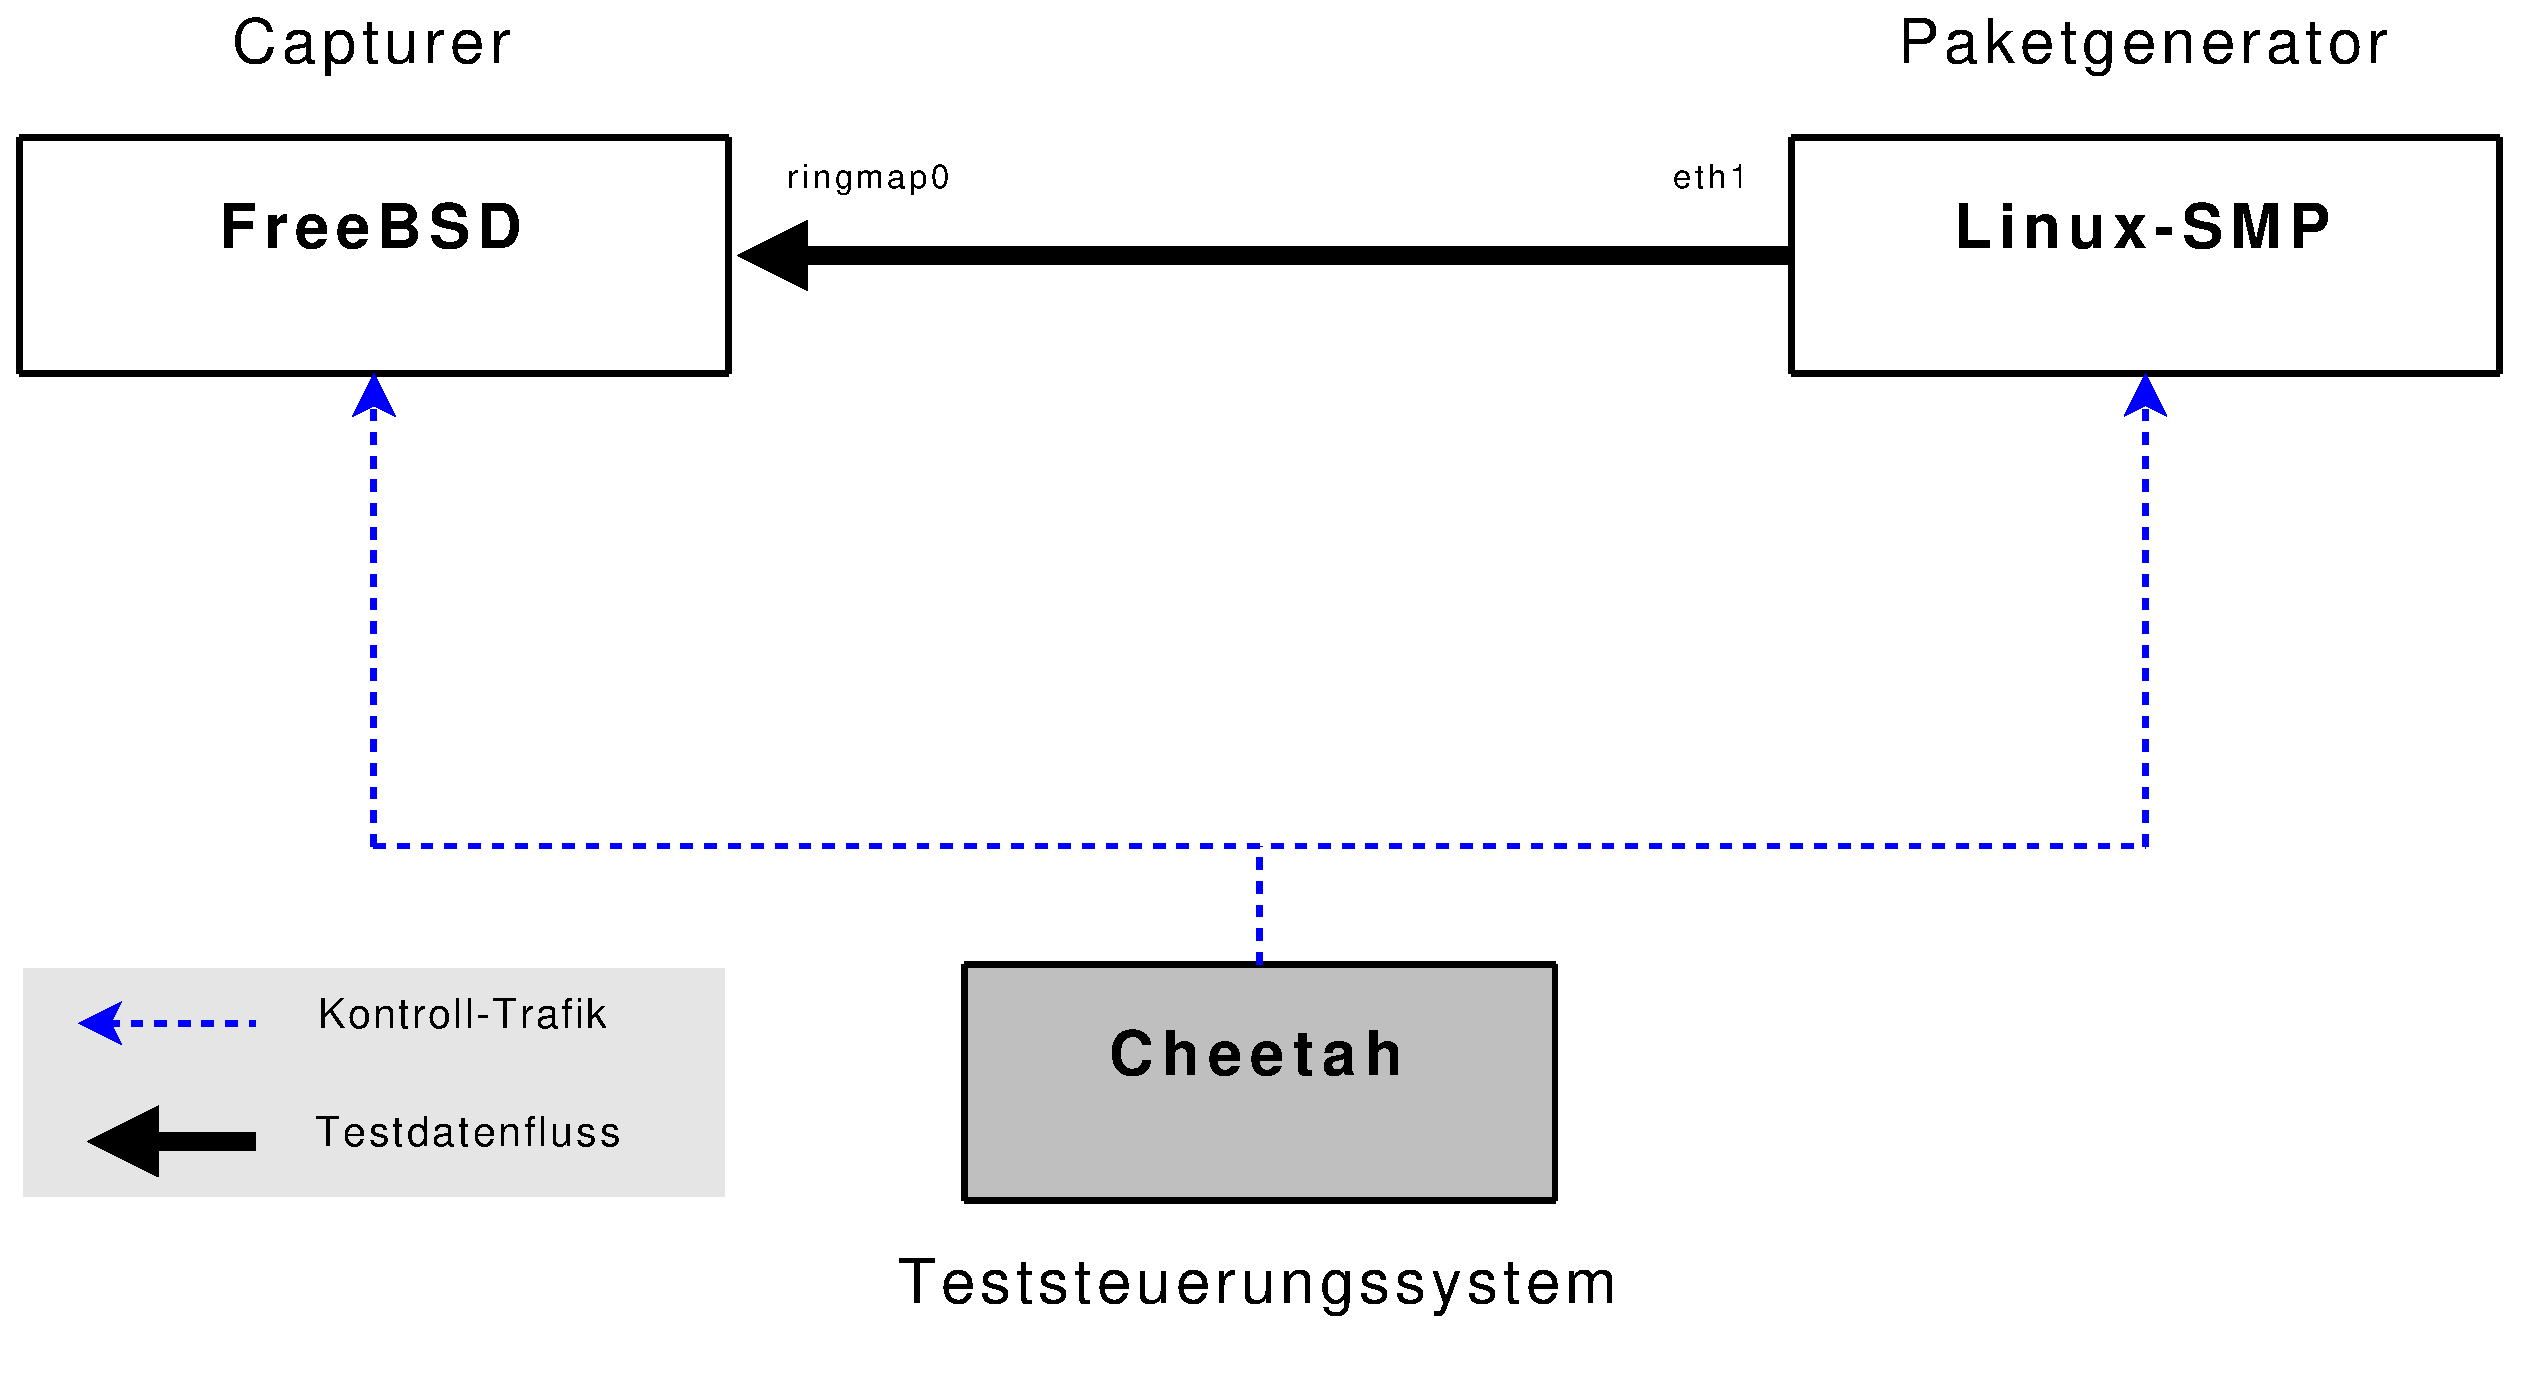
\includegraphics[width=5.5in]{bilder/Messaufbau}
\caption{Netzwerk-Diagramm des Testsbeds}
\label{img:test_aufbau}
\end{figure}
In diesem Kapitel werden die Ergebnisse des Leistungsvergleichs zwischen den
\emph{generischen} und den im Rahmen des Projektes entwickelten
\emph{ringmap}-Packet-Capturing-Stacks dargestellt. Für die Tests ist ein
Netzwerk mit drei Hosts aufgebaut. Das Netzwerkdiagramm der Testsumgebung ist
in Abbildung \ref{img:test_aufbau} dargestellt. Auf dem \textbf{Paketgenerator}
ist Verkehr mit unterschiedlichen Charakteristiken erzeugt und auf dem
\textbf{Capturer} erfasst. Dabei sind die Paketverluste und die
Systemlast während der Datenerfassung gemessen.
%
\ifthenelse{\boolean{BRIEF}}{}{   
Das \emph{ringmap}-Stack wird nicht nur mit unterschiedlichen Verkehrsmustern
untersucht. Für die Teststabläufe werden verschiedene Konfigurationsparameter
für das Betriebssystem und den Treiber eingesetzt, mit dem Ziel eine optimale
\emph{ringmap}-Konfiguration, die eine bestmögliche Leistung ermöglicht,
herauszufinden.\\\\
%
Die Performance des \emph{generischen} Stacks wurde bereits in mehreren
wissenschaftlichen Experimenten untersucht~\cite{fabian_da, pcin10gb_paper,
perfev_paper}. Aus diesem Grund werden mit dem \emph{generischen}-Stack nur
wenige Experimente durchgeführt, um die Performance von \emph{ringmap} und
\emph{generic} vergleichen zu können.
}

\subsection{Messaufbau}\label{sec:messaufbau}
Im Folgenden beschreibe ich die für Tests eingesetzten Knoten (Abbildung
\ref{img:test_aufbau}): 
\begin{itemize}
	\item Paketgenerator
		\begin{itemize}
			\item Ein leistungsfähigen Rechner zum Generieren des Test-Verkehrs.
			\item OS: Linux-SMP
			\item Linux Kernel Packet generator~\cite{linux_pktgen} wird für
				die Generierung des Netzverkehrs benutzt.
		\end{itemize}
	\item Capturer
		\begin{itemize}
			\item OS: FreeBSD mit \emph{generic} und \emph{ringmap}
				\begin{itemize}
					\item FreeBSD-7.2, i386-Kernel (32 Bit)
					\item Interrupt-Throttling default Parameter:
						\begin{itemize}
							\item 8000 Interrupts pro Sekunde maximal
						\end{itemize}
				\end{itemize}
			\item Hardware:
				\begin{enumerate}
					\item FreeBSD-1:
						\begin{itemize}
							\item \textbf{CPU:} AMD Athlon(tm) 64 Processor 2214.45-MHz
							\item \textbf{Netzwerkadapter:} PCI, Intel Dual Port Gigabit Ethernet Controller
						\end{itemize}
					\item FreeBSD-2:
						\begin{itemize}
							\item \textbf{CPU:} 4 x Intel(R) Xeon(R) CPU 1.60GHz
							\item \textbf{Netzwerkadapter:} PCIe, Intel HP NC360T PCIe DP Gigabit Server Adapter	 
						\end{itemize}
				\end{enumerate}
						\end{itemize}
	\item Teststeuerungssystem
		\begin{itemize}
			\item OS: Linux
			\item Scripte zur Teststeuerung.
		\end{itemize}
\end{itemize}
\ifthenelse{\boolean{BRIEF}}{}{  
\begin{figure} 
\centering 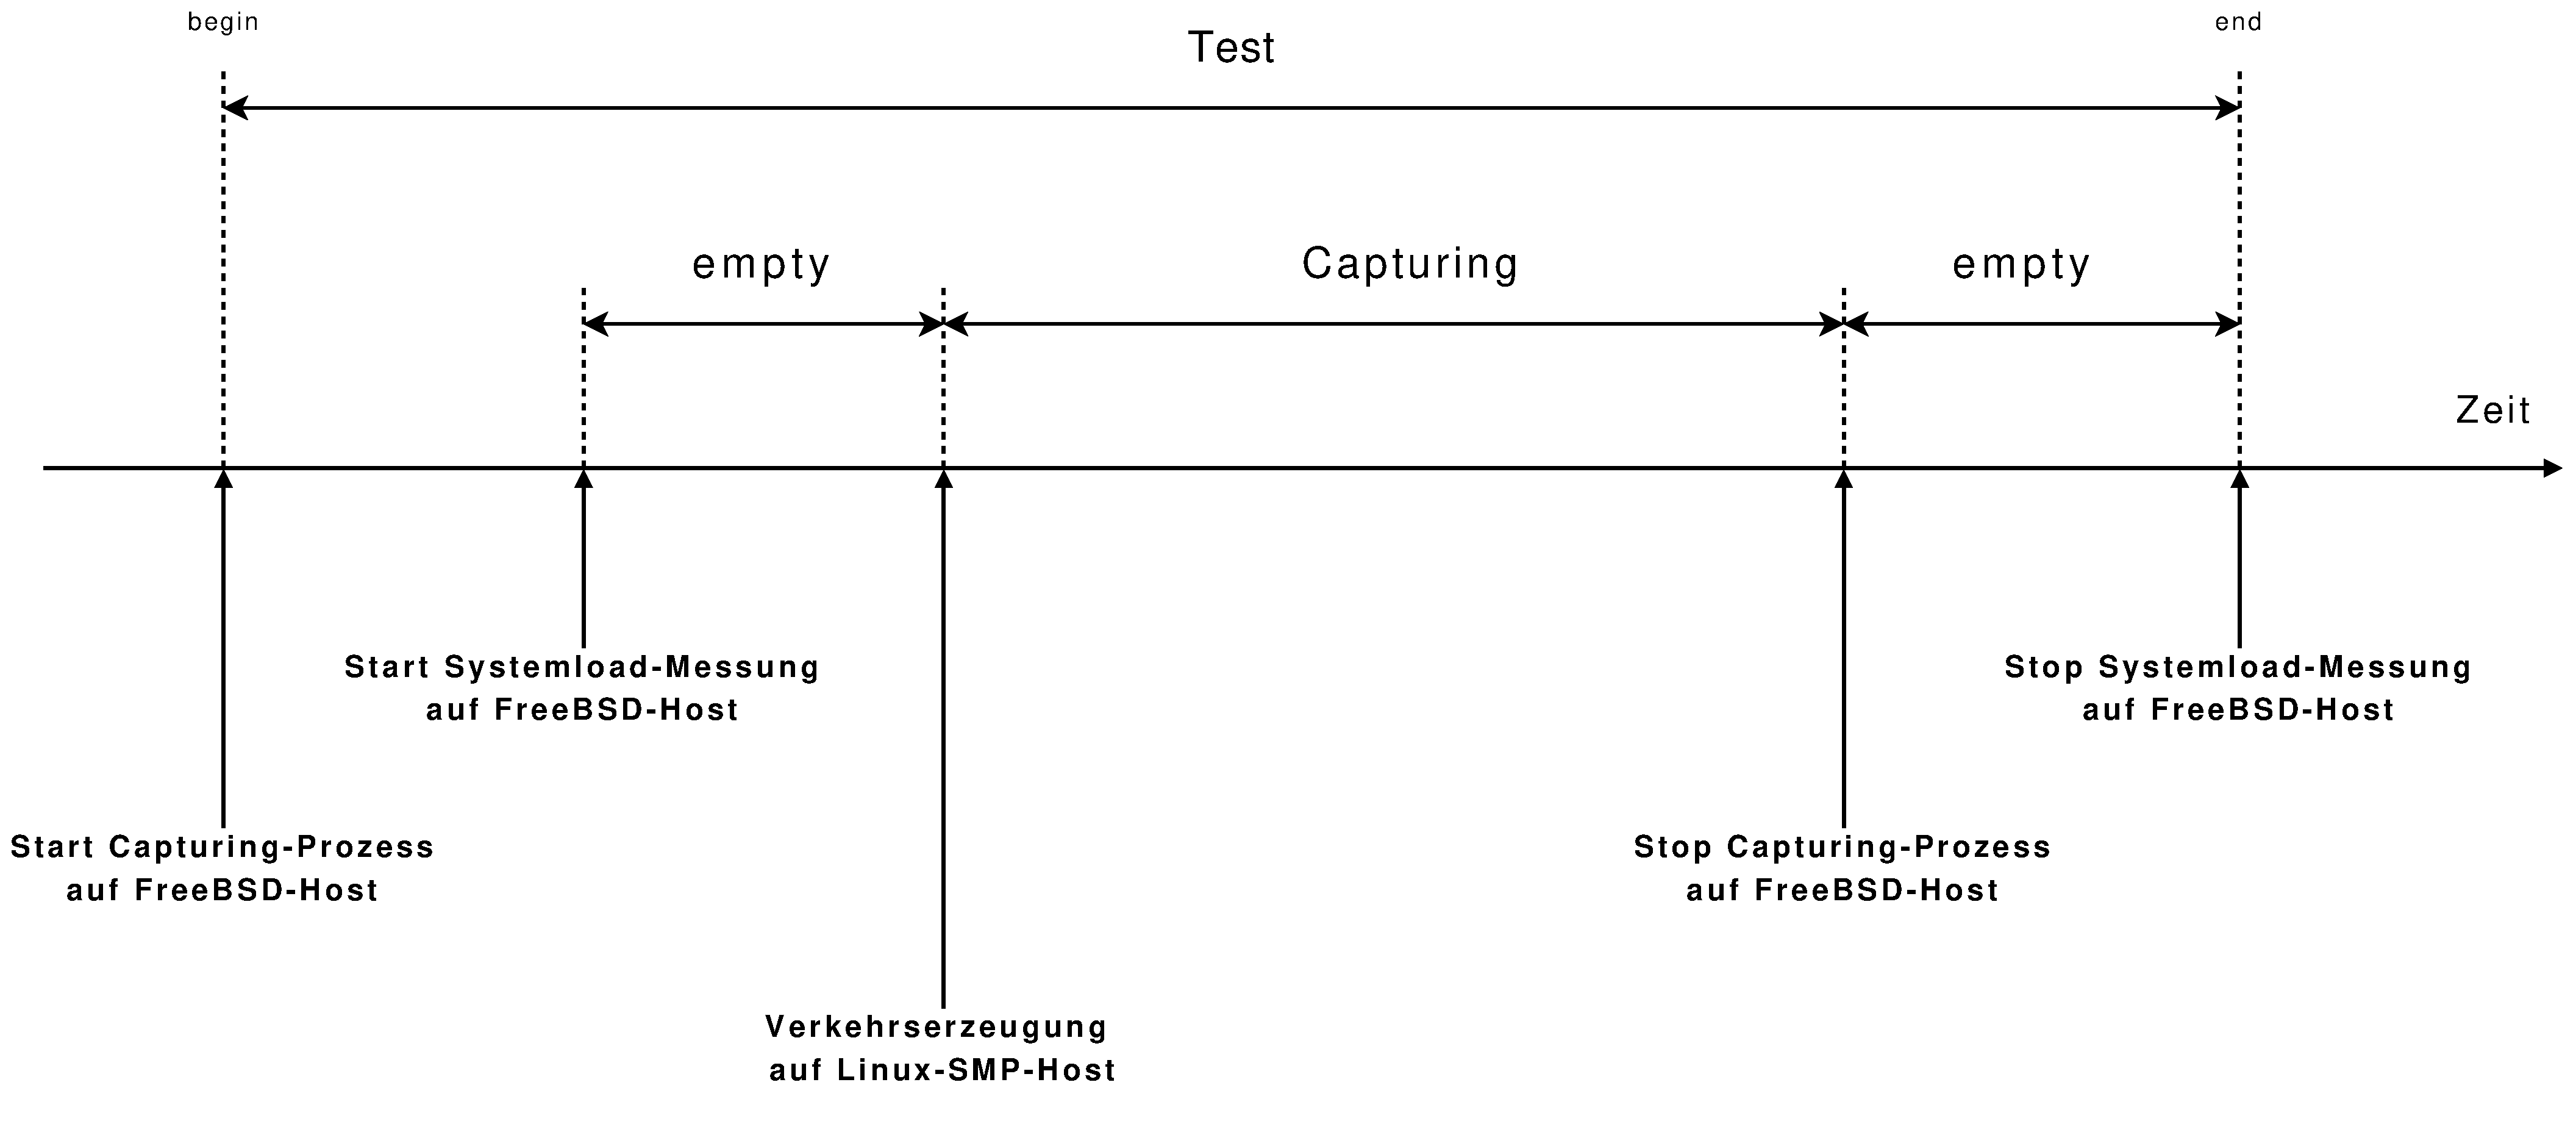
\includegraphics[width=6.5in]{bilder/Test_Zeit_Ablauf}
\caption{Testablauf}
\label{img:test_ablauf}
\end{figure}
\subsubsection{Testablaufspezifikationen}
Für die Testablauf-Steuerung wird ein Shellskript\footnote{SVN-URL:
\url{https://svn.net.t-labs.tu-berlin.de/svn/alexandre-da/src/70/scripts/dotests.sh}}
eingesetzt. Der Skript wird auf \emph{Cheetah} gestartet, und steuert durch
SSH-Verbindungen zu \emph{Capturer}- und \emph{Paketgenerator}-Host den Ablauf
jedes Testes.\\\\
Folgend beschreibe ich den Ablauf der Tests in Einzelschritten (siehe Abbildung
\ref{img:test_ablauf}): 
\begin{enumerate}
	\item SSH-Login auf \emph{FreeBSD}:
		\begin{enumerate}
			\item Starten Capturing-Prozess.
			\item Starten Systemload-Messung.
		\end{enumerate}
	\item SSH-Login auf \emph{Linux-SMP}:
		\begin{enumerate}
			\item Starten Verkehrserzeugung-Prozess
				\begin{itemize}
					\item Es wird Testdatenfluss generiert. Dabei wird eine
						bestimmte Anzahl von Paketen gleicher Länge erzeugt und
						zu dem \emph{Capturer} gesendet.
				\end{itemize}
			\item Speichern in einer Temp-Datei der Charakteristiken des
				erzeugten Verkehr: Bit-Rate, Paket-Rate.
		\end{enumerate}
	\item SSH-Login auf \emph{FreeBSD}:
		\begin{enumerate}
			\item Stop Capturing-Prozess
			\item Stop Systemload-Messung.
			\item Speichern in einer Temp-Datei der Systemload-Mess-Daten und
				Anzahl der empfangenen Pakete. 
		\end{enumerate}
	\item SSH-Login auf \emph{FreeBSD} und \emph{Linux-SMP}:
		\begin{itemize}
			\item Kopieren der gespeicherten Test-Daten von den \emph{FreeBSD} und
			\emph{Linux-SMP} auf \emph{Cheetah}
		\end{itemize}
\end{enumerate}
Jeder Test wird fünf mal wiederholt. Für die gemessenen Werte wird das
Arithmetisches Mittel und Standardabweichung berechnet, welche auf den Grafiken
in den folgenden Abschnitten dargestellt sind.

}
\subsubsection{Erzeugung von Verkehr}
Der Verkehr für die Tests wird mit
\emph{Linux-Kernel-Packet-Generator}(\emph{pktgen})~\cite{linux_pktgen} erzeugt.
\emph{pktgen} ist ein Linux-Kernel-Module, das benutzt wird um die UDP-Pakete
zu generieren und diese ins Netz zu senden. Für die Steuerung von \emph{pktgen}
wird das \verb+/proc+-Filesystem benutzt.\\\\
Der \emph{Linux-Kernel-Paket-Generator} wurde für die Experimente ausgewählt,
weil er mehrere Vorteile mit dem Unterschied zu den anderen Software (z.B.
Nemesis, Scapy, Iperf, etc\ldots) für die Erzeugung des Netz-Verkehr bietet. Vor
allem handelt es sich dabei um eine sehr hohe Paket-Rate, die mit \emph{pktgen}
erzeugt werden kann.
%
\ifthenelse{\boolean{BRIEF}}{}{  
Um eine hohe Paket-Rate bei Intel Ethernet Gigabit Adapter zu erzeugen, müssen
einige Eigenschaften des Netzwerkadapters beachtet werden, und zwar,
handelt es sich um \emph{Flow-Control}-Mechanismus.
}
%
\ifthenelse{\boolean{BRIEF}}{}{   
\subsubsection*{Flow-Control}
Unter dem Begriff \emph{Flow-Control} verstecken sich unterschiedliche 
Verfahren, die es erlauben, die Datenübertragung in einem Netz, die nicht synchron 
abläuft, so zu steuern, dass eine möglichst kontinuierliche Datenübermittlung ohne 
Paket-Verluste erfolgen kann. Das erfolgt sich dadurch, dass die Paketsendung 
im Fall eines schnelles Senders und eines langsamen Empfänger zeitweise unterbrochen 
wird.\\\\
%
Beim Intel Gigabit Netzwerkadapter ist der \emph{Flow-Control}-Mechanismus per Default
eingeschaltet, und das kann  bei der Verkehr-Generierung zu einigen  Problemen
führen. Erstens wird der \emph{Flow-Control}-Verkehr nicht von der
Capturing-Software wahrgenommen, benutzt aber Bandbreite, die wir für unsere
Test-Abläufe maximal benutzen wollen.  Zweitens, da unser Ziel im Erreichen
maximal hohe Paket-Rate liegt, ist in unserem Fall der \emph{Flow-Control} nur ein
Hindernis, der die Datentransferrate begrenzt. Deshalb muss es vor Beginn der
Experimente sowohl auf dem Capturing-Host, als auch auf dem
Paket-Generator-Host ausgeschaltet werden.
%
\subsubsection*{Ausschalten von Flow-Control auf dem Intel Gigabit Netzwerkadapter}
Unter Linux kann die Abschaltung von \emph{Flow-Control} beim Laden des
\emph{pktgen}-Modules an der Kommandozeile erfolgen: 
\begin{equation}
	\verb+# modprobe e1000 FlowControl=0+
\end{equation}
Unter FreeBSD wird \emph{Flow-Control} aus dem Treiber durch direkte Beschreibung 
des \emph{Receive-Control-Register} (\verb+RCTL+) ausgeschaltet (Listing \ref{code:flow_ctl_dis}):
\begin{lstlisting}[frame=single, caption={Funktion zur Ausschaltung des Flow-Control-Mechanismus. Die Funktion wird im ringmap-Treiber verwendet.}, captionpos={b}, label={code:flow_ctl_dis}]
void ringmap_disable_flowcontr(struct adapter *adapter)
{
	unsigned int ctrl; 
	ctrl = E1000_READ_REG(&(adapter)->hw, E1000_CTRL);
	ctrl &= (~(E1000_CTRL_TFCE | E1000_CTRL_RFCE));
	E1000_WRITE_REG(&(adapter)->hw, E1000_CTRL, ctrl);
}
\end{lstlisting}	
%
}
\subsubsection{Messung der CPU-Auslastung und der Paketverluste beim Capturing}
Auf dem FreeBSD-Host werden beim Test-Ablauf die auf dem Paketgenerator
generierten und gesendeten Pakete erfasst. Dabei wird die Anzahl der
empfangenen Pakete und die Systemload beim Capturing auf dem Capturer gemessen.
Bei allen Experimenten werden die erfasste Pakete nicht auf die Festplatte 
geschrieben, sondern nur im RAM gezählt.
%
\subsubsection*{Messung von Paketverlusten}
Für das Packet-Capturing wird eine einfache Anwendung implementiert, die für den
Paketzugriff die Bibliothek \emph{Libpcap} benutzt. In dieser Capturing-Anwendung ist
ein \emph{callback}-Funktion enthalten, die für jedes empfangene Paket
aufgerufen wird, und derer Aufgabe ist es, die empfangene Pakete zu zählen.
Das Paketverlust (\begin{math}P_{los}\end{math}) wird als Differenz zwischen 
den Anzahl der empfangenen (\begin{math}P_{rcv}\end{math}) und
der gesendeten Pakete (\begin{math}P_{send}\end{math}) berechnet:
	\begin{equation}
		P_{los} = P_{send} - P_{rcv}
		\label{equ:pktloss}
	\end{equation}
%
\subsubsection*{Messung von CPU-Auslastung}
Die CPU-Last wird auf FreeBSD über die \emph{sysctl}-Variable
\lstset{language=bash} \verb+kern.cp_time+ abgefragt:
\begin{lstlisting}[captionpos={b}, frame=single]
% sysctl kern.cp_time
kern.cp_times: 27281 1333 301046 513 1001093319
%
\end{lstlisting}
Bei der Abfrage der \verb+kern.cp_time+-Variable werden auf dem Standard-Output die Zeiten
ausgegeben, welche die CPUs seit dem Start des Betriebssystem jeweils im \verb+user+-,  
\verb+nice+-, \verb+syst+-, \verb+intr+- und \verb+idle+-Modus verbracht
haben.\\\\
Beim Präsentieren der Tests-Ergebnisse wird aber nicht die volle CPU-Last, die
aus den \verb+user+- \verb+nice+- \verb+syst+- \verb+intr+- \verb+idle+-Load
besteht, sondern lediglich die \textbf{Systemload} (\verb+syst+) angegeben.  Da
die Implementierung des neuen Stack hauptsächlich Kernel-Code betrifft,
interessiert uns vor allem die Systemload (\verb+syst+)\footnote{Aufgrund der
default Treiber-Einstellungen für Interrupt-Moderation, bleibt intr-Load
konstant. Deshalb interessiert uns Interrupt-Load auch nicht}.  Der Absicht der
Tests ist das Prüfen, ob unsere Entwurf-Ansätze korrekt sind, und ob sie zu dem
gewünschten Ziel führen. Anders gesagt, zu prüfen, ob die Ausführung des
Kernel-Codes vom neuen \emph{ringmap}-Capturing-Stack eine niedrigere
Systemlast als beim \emph{generic}-Capturing-Stack verursacht.
%
\ifthenelse{\boolean{BRIEF}}{}{   
Im System-Mode wird auch die Interrupt-Service-Routine(ISR) des Netzwerkadapters
ausgeführt (siehe Abschnitt \ref{sec:intr_behandlung}). Weil bei allen Tests
für die Interrupt-Rate-Steuerung \emph{Interrupt-Throttling} (siehe
Abschnitt \ref{sec:intr_coal}) verwendet wurde, blieb die Interrupt-Rate
während unserer Tests immer konstant, was auch immer eine konstante
Interrupt-Load (\verb+intr+: etwa $3\%$) verursacht hat. Aus diesem Grund 
können wir die Interrupt-Load in unseren Vergleichen ignorieren.
%liegt die Präsenz der Interrupt-Load auch außerhalb unserer Interessen.
%
\subsubsection*{Systemload-Messung}
Um die \textbf{Systemload} (\verb+syst+) während eines Test-Ablaufs zu messen, werden
die Werte des \verb+syst+-Counters vor Begin des Tests
(\begin{math}t_{begin}\end{math}) und nach dem Test (\begin{math}t_{end}\end{math}) 
gespeichert.  Durch die Differenz ergibt sich 
die Zeit, die CPUs während des Tests mit dem Ausführen des \verb+syst+-Codes zugebracht haben.  Diese Zeit entspricht aber nicht
exakt dem Testablauf, denn es sowohl zwischen den Messungsbeginn und Capturing
als auch zwischen Capturing-End und dem Mess-Ende (kurze)
Zeitintervalle (\begin{math}t_{empty}\end{math}) gibt, in
denen der \verb+syst+-Counter Zeit-Statistiken sammelt, die nicht während
Capturing entstehen, was das Endergebnis etwas verfälscht (siehe Abbildung \ref{img:test_ablauf}). \begin{math}t_{empty}\end{math} lässt sich messen, 
und zwar dadurch, dass man einen Test ohne Paketversand veranstaltet.\\\\
%
Aber dadurch, dass das Auftreten der Ereignisse, die das Ausführen des
Kernel-Codes verursachen (z.B. Interrupts oder Traps) unvorhersagbar ist, und,
dass die Anzahl von solchen Ereignissen pro Zeitintervall meistens variabel
bleibt, ist dieser Wert nicht exakt bestimmbar. Daher wurden vor Beginn aller Tests mehrere Messungen von 
\begin{math}t_{empty}\end{math} gemacht und ein durchschnittliches Wert 
\begin{math}\tilde{t}_{empty}\end{math}  berechnet.\\\\
%
Dann berechnet sich die Zeit (\begin{math}T_{syst}\end{math}), 
die sich CPUs während des Capturing im 
\verb+syst+-Mode verbracht haben durch: 
\begin{equation}
	T_{syst} = t_{end} - t_{begin} - \tilde{t}_{empty}
\end{equation}
Auf gleiche Weise lassen sich die CPU-Zeiten für \verb+user+- \verb+nice+- \verb+idle+- und \verb+intr+-Mode
berechnen. Dann berechnet sich die \textbf{Systemload} ($S$) als der prozentuelle Zeitanteil,
den die CPUs im \verb+syst+-Mode während des Tests verbracht haben 
durch:
\begin{equation}
	S = \frac{T_{syst} * 100}{(T_{user} + T_{nice} + T_{syst} + T_{intr} + T_{idle})}
\end{equation}

\subsection{Test-Parameter}\label{sec:test_params}
Für jeden Testablauf werden unterschiedliche Parameter eingesetzt, die sowohl
den Paket-Generierungs-Prozess als auch den Capturing-Prozess beeinflussen. Für
die Tests, die zum Vergleich des \emph{generic}- und \emph{ringmap}-Capturing-Stacks durchgeführt
wurden, werden lediglich die Paket-Generator-Parameter geändert, während die
Konfiguration der Treiber auf dem Capturing-Host konstant blieb.\\\\
Für die Auswertung der Performance des \emph{ringmap}-Stack wird eine größere 
Menge an Tests durchgeführt, um eine Konfiguration herauszufinden, bei der 
\emph{ringmap}-Stack mit optimaler Performance funktioniert.

\subsubsection{Parameter für die Generierung des Netz-Verkehrs}
Die Parameter, die für \emph{Linux Kernel Pakete Generator} gesetzt werden, 
erlauben es, die Paket-Größe und die Paket-Rate (dadurch auch Bit-Rate)
des generierten Verkehr zu steuern. Die Konfiguration von \emph{pktgen}
läuft über das \verb+/proc+-Filesystem ab.\\\\
In den Tests wurden folgende \emph{pktgen}-Parameter
eingesetzt\footnote{Eine detailierte Beschreibung der \emph{pktgen}-Parameter findet sich in
der Dokumentation~\cite{linux_pktgen}}:
\begin{description}
\item \verb+pkt_size+	
	\begin{itemize}
		\item Die Länge der erzeugten und gesendete Pakete. Beeinflusst auch 
			die Paket- und Bit-Rate des Verkehrs, denn je kleiner die Pakete sind ,
			desto größer wird der CPU-Aufwand für das Erzeugen einer bestimmten Datenmenge
			und desto höher die Anzahl der Bus-Transaktionen um diese Datenmenge 
			vom RAM zum Netzwerkadapter transferieren und ins Netz zu senden.
	\end{itemize}
\item  \verb+dstmac+	
	\begin{itemize}
		\item  Destination-MAC-Adresse. Wurde bei den Tests des
			\emph{generic}-Capturing-Stack absichtlich auf eine nicht dem NIC
			entsprechende MAC-Adresse gesetzt, damit die empfangenen Pakete
			nicht vom Protokoll-Stack bearbeitet werden, und dadurch keine
			zusätzliche Systemload beim Capturing erzeugen. 
	\end{itemize}
\item  \verb+delay+
	\begin{itemize}
		\item Zeitintervall in Nanosekunden zwischen den gesendeten Paketen.
			Beeinflusst die Paket- und damit auch die Bit-Rate des erzeugten
			Verkehr.
	\end{itemize}
\item  \verb+count+
	\begin{itemize}
		\item Anzahl der zu erzeugenden und zu sendenden Pakete. 	
	\end{itemize}
\end{description}

\subsubsection{Treiber-Parameter}
Die Parameter die für den \emph{ringmap}-Treiber gesetzt werden, beeinflussen
seine Performance, und können dadurch auf die Capturing-Performance einwirken.
Einige Parameter werden über \emph{sysctl}-Befehl~\cite{man_sysctl} gesetzt,
die anderen aber nur als Makrodefinitionen im Source-Code.
%
\begin{description}
	\item \verb+SLOTS_NUMBER+
		\begin{itemize}
			\item Ringpuffer-Größe: Anzahl der Ring-Slots bzw. der
				Paket-Puffer. Wird als Makrodefinition in der Datei
				\verb+fiveg_da.h+\footnote{\url{https://svn.net.t-labs.tu-berlin.de/svn/alexandre-da/src/70/em/fiveg_da.h}} gesetzt.
		\end{itemize}
	\item \verb+rx_processing_limit+
		\begin{itemize}
			\item Die maximale Anzahl der Pakete, die ein von der ISR geplanter
				Kernel-Thread bearbeiten darf. Wird über \emph{sysctl}-Befehl
				gesetzt. 
		\end{itemize}
\end{description}
}
\subsection{Ergebnisse}\label{sec:test_ergebnisse}
In diesem Kapitel werden die Ergebnisse der im Rahmen des Projektes
durchgeführten Experimente dargestellt. Der erste Abschnitt stellt die
Ergebnisse der Experimente mit dem neuen \emph{ringmap}-Packet-Capturing-Stacks dar. Es
werden die Systemload und Paketverluste beim Capturing in Abhängigkeit von der
Date-Rate des Verkehrs und der anderen Parameter dargestellt.\\\\
% 
Im Abschnitt \ref{sec:erg_verg} vergleichen wir die Performance des ringmap-
mit dem generic-Capturing-Stack, um den Performance-Gewinn durch den neuen
\emph{ringmap}-Capturing-Stack quantitativ zu bestimmen.

\subsubsection{Ringmap-Paket-Capturing-Stack}\label{sec:erg_ringmap_stack}
In diesem Abschnitt sind die Ergebnisse der Experimenten mit \emph{ringmap}-Capturing-Stack
dargestellt. Das Ziel der Experimenten die Capturing-Performance des \emph{ringmap}-Stacks 
in Abhängigkeit von den folgenden Parameter herauszufinden:
\begin{itemize}
\ifthenelse{\boolean{BRIEF}}{}{   
	\item Treiber-Konfigurationsparameter: \verb+rx_processing_limit+, \verb+SLOTS_NUMBER+.
}
	\item Paket-Ringpuffer-Größe
	\item Daten-Rate des erfassten Verkehr.
\end{itemize}

\subsubsection*{Paketverluste in Abhängigkeit von der Anzahl der Slots im  Paket-Ringpuffer}
\textbf{Das Ziel} dieses Experiments ist es, die Abhängigkeit der Paketverluste
während Capturing von der Größe des Paket-Ringpuffers (Ring-Buffer)
herauszufinden. In diesem Experiment ist eine Reihe von Tests durchgeführt. Für
alle Tests ist der Verkehr mit den kleinsten 64-Bytes Pakete und mit der maximal
erreichbaren Bit-Rate (c.a. $696Mbit/sec$) generiert.
%
\begin{itemize}
\item Konfiguration auf dem Capturer: 
\begin{itemize}
	\item \textbf{Hardware:} FreeBSD-2 (PCIe)
	\item \textbf{Betriebssystem:} FreeBSD \textbf{7.2}, \textbf{non-SMP Kernel}
\end{itemize}
\item Verkehrsparameter:
\begin{itemize}
	\item Paketlänge: 64-Bytes
	\item Paketmenge: 15000000
	\item Bit-Rate: etwa $696MB/sec$
\end{itemize}
\end{itemize}
\begin{figure} 
\centering 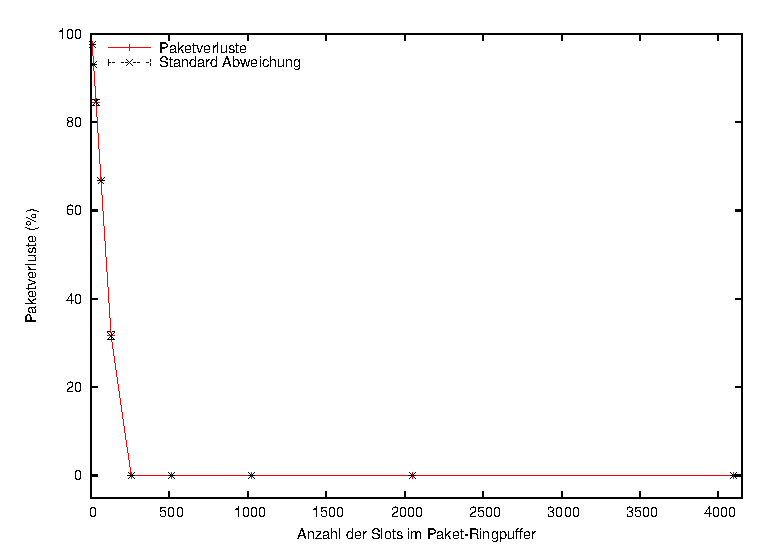
\includegraphics[width=5.5in]{plots/graphs/pktlos_single_bufsize.eps}
\caption{Paketverluste in Abhängigkeit von der Anzahl der Slots im Paket-Ringpuffer}
\label{img:plot_pktlos_puffs}
\end{figure}
%
\ifthenelse{\boolean{BRIEF}}{}{   
Beil allen durchgeführten Tests wird der Wert von \verb+rx_processing_limit+
auf $200$ gesetzt und der Wert \verb+SLOTS_NUMBER+ zwischen 8 und 4096
geändert. 
}
% 
\paragraph*{Paketverluste:}
In Abbildung \ref{img:plot_pktlos_puffs} sind die Paketverluste während
Capturing dargestellt.  Auf der X-Achse wird die Anzahl der Slots im
Ring-Buffer dargestellt.  Auf der Y-Achse die prozentuelle Anzahl der
Paketverluste. In allen durchgeführten Experimenten mit 256 oder mehr
Paket-Slots sind die Paketverluste relativ konstant und liegen unter $0.02\%$,
d.h. die Erhöhung der Anzahl der Slots ab 256 bringt keinen weiteren Gewinn
mehr. 
%
\ifthenelse{\boolean{BRIEF}}{}{   
\subsubsection*{Performance in Abhängigkeit von der maximalen Anzahl der pro Kernel-
Thread-Ablauf bearbeitende Paketen: rx\_processing\_limit}
\textbf{Das Ziel} dieses Experiments ist es, die optimale Werte für die
Variable \verb+rx_processing_limit+ zu finden, bei welchen die Paketverluste
und die Systemload minimal sind.\\\\
%
Konfiguration auf dem Capturer (\verb+FreeBSD+-Host): 
\begin{itemize}
	\item \textbf{Hardware:} FreeBSD-2	
	\item \textbf{Betriebssystem:} FreeBSD \textbf{7.2}, \textbf{single-CPU-Kernel}
	\item \textbf{Treiber:} 
		\begin{itemize}
			\item Paket-Ringpuffer-Größe: \verb+SLOTS_NUMBER+$=1024$
			\item Bit-Rate: etwa $696MB/sec$
		\end{itemize}
\end{itemize}
Verkehrsparameter:
\begin{itemize}
	\item Paketlänge: 64-Bytes
	\item Paketmenge: 15000000
\end{itemize} 
\begin{figure} 
\centering 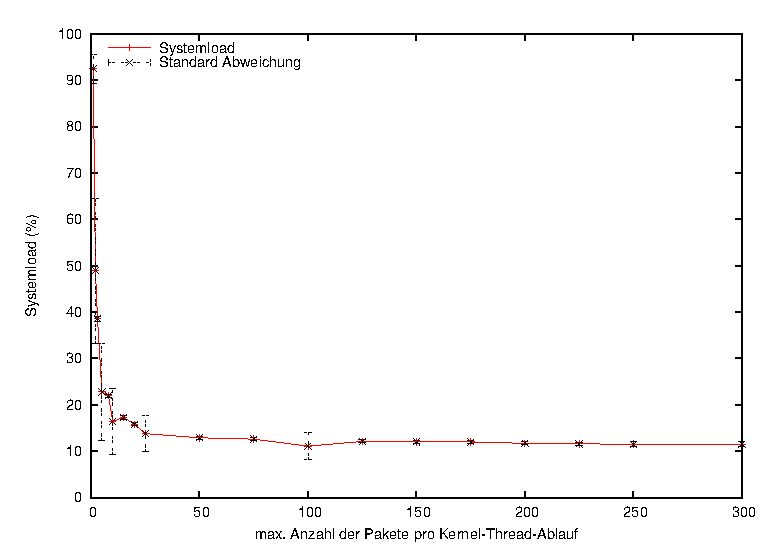
\includegraphics[width=5.5in]{plots/graphs/sysload_single_kts}
\caption{Systemload in Abhängigkeit von der maximalen Anzahl der pro Kernel-Thread-Ablauf
bearbeitende Pakete}
\label{img:plot_sysload_kts}
\end{figure} 
Bei Experimenten wird der wert von \verb+rx_processing_limit+ zwischen 1 und 300 
geändert.
\paragraph*{Paketverluste:} 
Bei allen durchgeführten Experimenten ergibt sich ein sehr kleiner Paketverlust
geringer als $0.02\%$ aller generierten Pakete.
\paragraph*{Soystemload:}
Die Ergebnisse des Systemload-Messungs-Experimentes sind in Abbildung
\ref{img:plot_sysload_kts} dargestellt.  Auf der X-Achse werden die Werte der
Variable \verb+rx_processing_limit+ dargestellt, auf der Y-Achse die Systemload
bei der Verkehrserfassung. Eine hohe Anzahl von Paketen pro Ablauf des
Kernel-Threads verursacht eine geringe Systemlast. Unsere Messungen zeigen dass
bei einer Einstellung $>50$ die Systemlast relativ Konstant unter $12\%$ bleibt. 
Die weitere Erhöhung des Wertes bringt keinen Gewinn mehr.
}
\subsubsection*{Performance in Abhängigkeit von Paketlänge, Bit-Rate und Paket-Rate}
\textbf{Das Ziel} des Experiments ist es, die Abhängigkeit der
Capturing-Performance von der Paketsgröße und Daten-Rate im Netzverkehr
herauszufinden.
%
\begin{itemize}
\item Konfiguration auf dem Capturer: 
\begin{itemize}
	\item \textbf{Hardware:} FreeBSD-2
	\item \textbf{Betriebssystem:} FreeBSD \textbf{7.2}, \textbf{non-SMP Kernel}
	\item \textbf{Treiber:} 
		\begin{itemize}
			\item Paket-Ringpuffer-Größe: 1024 Slots
		\end{itemize}
\end{itemize}
\item Verkehrsparameter:
\begin{itemize}
	\item Paketlängen: 64- , 200-, 300-Bytes
	\item Paketmengen: 15000000
\end{itemize}
\end{itemize}
%
\paragraph*{Paketverluste:} Bei allen Experimenten ergibt sich für Paketgrößen
über 200 Bytes die Paketerfassungsrate $100\%$. Nur in den Experimenten mit der
kleinsten Paketgröße von 64-Bytes und nur bei der höchsten erreichte Bit-Rate
von $627 MB/sec$ ergibt sich ein sehr kleines Paketverlust geringer als
$0.02\%$ aller generierten Pakete.
%
\paragraph*{Systemload:}
Die Ergebnisse der Systemload-Messung werden in den Abbildungen
\ref{img:plot_sysload_mbs} und \ref{img:plot_sysload_pps} dargestellt. Die
maximal erreichte Systemload beim Capturing in allen Experimenten liegt unter
$12\%$ und wird erreicht beim Capturing des Verkehrs mit den kleinsten
64-Bytes-Paketen.\\\\
%
In Abbildung \ref{img:plot_sysload_pps} wird die Systemload in Abhängigkeit von
der Paket-Rate dargestellt. Bei diesen Ergebnissen kann man deutlich sehen,
dass die Systemload beim Capturing von der Paket-Rate und nicht von der
Paket-Größe beeinflusst wird. Drei Verkehrsströme mit unterschiedlichen
Paketgrößen verursachen fast identisch gleiche Systemload (die Unterschiede
sind geringer als $0.5\%$) wenn die Paketraten in diesen drei Verkehrsströmen
gleich sind.  Dies lässt sich einfach erklären. Im neuen \emph{ringmap}-Treiber
wurden alle Paket-Kopie-Operationen und Speicherallozierungen entfernt. Der
Userspace-Prozess bekommt den Zugriff auf die Pakete sofort nach dem
DMA-Transfer. Aus diesen Gründen wird beim Capturing mit dem
\emph{ringmap}-Treiber im Kernelspace die geringstmögliche Arbeit erledigt, die
pro Paket-Puffer skaliert und nicht von der Paket-Größe abhängt.
%
\begin{figure} 
\centering 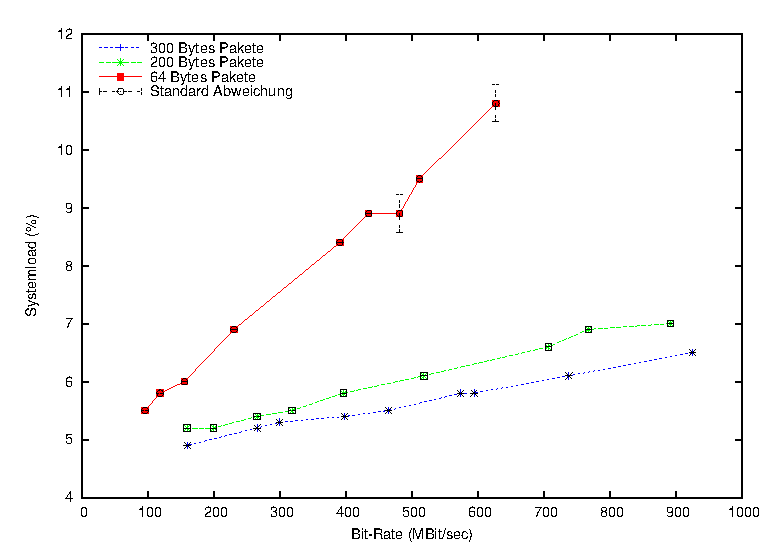
\includegraphics[width=5.5in]{plots/graphs/sysload_single_CPU_pcie_mbs}
\caption{Systemload in Abhängigkeit von Bit-Rate beim Capturing}
\label{img:plot_sysload_mbs}
\end{figure}
\begin{figure} 
\centering 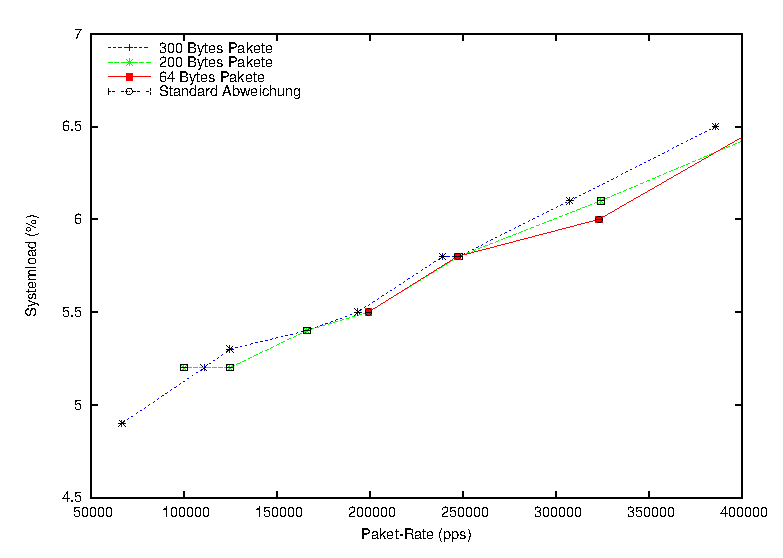
\includegraphics[width=5.5in]{plots/graphs/sysload_single_CPU_pcie_pps}
\caption{Systemload in Abhängigkeit von Paket-Rate beim Capturing}
\label{img:plot_sysload_pps}
\end{figure}
%
\ifthenelse{\boolean{BRIEF}}{}{   
\subsubsection*{Performance in Abhängigkeit von der Anzahl der CPU's}
\textbf{Das Ziel} des Experiments ist es, die Paketverluste beim Capturing 
in Abhängigkeit von der Anzahl der CPUs auf dem Capturing-System zu messen.\\\\
%
Konfiguration auf dem Capturer (\verb+FreeBSD+-Host): 
\begin{itemize}
	\item \textbf{Hardware:} FreeBSD-2	
	\item \textbf{Betriebssystem:} FreeBSD \textbf{7.2}, \textbf{single-CPU-Kernel}, \textbf{SMP}-Kernel
	\item \textbf{Treiber:} 
		\begin{itemize}
			\item Paket-Ringpuffer-Größe: 1024 Slots
		\end{itemize}
\end{itemize}
Verkehrsparameter:
\begin{itemize}
	\item Paketlänge: 64-Bytes
	\item Paketmenge: 15000000
\end{itemize}
%
Bei diesem Experiment werden für das Capturing unterschiedliche FreeBSD-Kerne
eingesetzt.  Bei einem Experiment läuft das Capturing mit dem SMP-Kernel, bei
dem anderen wird ein Kernel ohne SMP-Funktionalität verwendet. Für beide Tests
wird der Verkehr aus 64-Byte-Paketen generiert und gesendet. Die Ergebnisse des
Experiments sind in Abbildung \ref{img:plot_pktlos_single_vs_smp_mbs} zu sehen.
Auf der X-Achse ist die generierte Datenrate dargestellt. Auf der Y-Achse die
absolute Zahl der Paketverluste. Die durchschnittliche Anzahl der Paketverluste
für die Experimente mit einem SMP-Kernrel wird mit blauen Plus-Zeichen, die mit
dem Single-Kernel mit grünen Quadraten dargestellt. Die Paketverluste sind in
beiden Fällen im Verhältnis zur generierten Paketrate gering, steigen im Fall
des SMP-Kernels aber ab 400MBit/s stark an, bis auf 800 verlorene Pakete pro
Experiment.\\\\ 
%
Der SMP-Kernel Zeigt etwas schlechteres Performance. Der Grund dafür kann ein
Datenlokalitäts-Problem sein. Die unterschiedliche CPU-Kerne haben mindestens
einen eigenen Daten-Cache-Level, was Cache-Misses bei der Datenbearbeitung
verursachen kann. Dies war wahrscheinlich der Grund für die höheren
Paketverluste auf dem SMP-System.  Dennoch ist die Systemload beim Capturing
mit einem Single-CPU-Kernel geringer als $12\%$. Das heißt, dass eine CPU
problemlos das Capturing des Verkehrs bis 1Gbit schafft.
\begin{figure} 
\centering 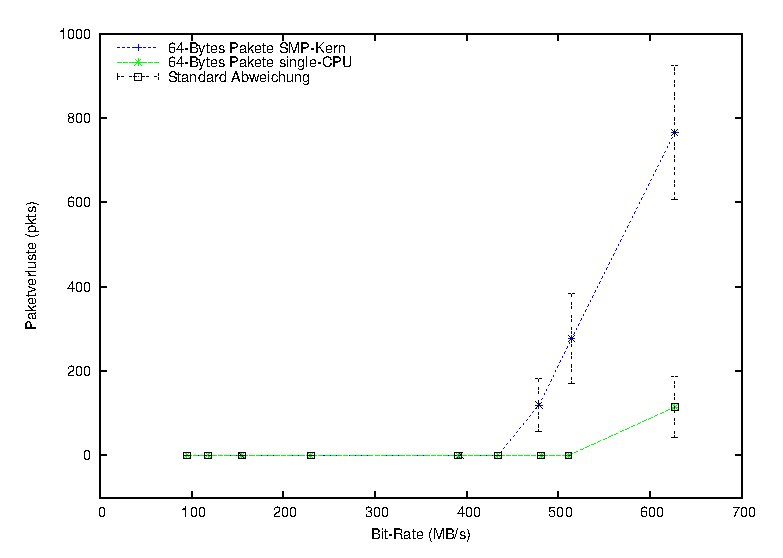
\includegraphics[width=5.5in]{plots/graphs/pktloss_single_vs_SMP_PCIe_mbs}
\caption{Paketverluste in Abhängigkeit von Paket-Rate beim Capturing auf einem SMP und single-CPU-System}
\label{img:plot_pktlos_single_vs_smp_mbs}
\end{figure}

\subsubsection*{Performance in Abhängigkeit von der PCI-Bus-Variante}
\textbf{Das Ziel} des Experimentes ist es die Capturing-Performance des
\emph{ringmap}-Stacks beim konventionellen PCI zu messen.\\\\
%
Konfiguration auf dem Capturer (\verb+FreeBSD+-Host): 
\begin{itemize}
	\item \textbf{Hardware:} FreeBSD-1
	\item \textbf{Betriebssystem:} FreeBSD \textbf{7.2}, \textbf{single-CPU-Kernel}
	\item \textbf{Treiber:} 
		\begin{itemize}
			\item Paket-Ringpuffer-Größe: 1024 Slots
		\end{itemize}
\end{itemize}
Verkehrsparameter:
\begin{itemize}
	\item Paketlänge: 64-Bytes
	\item Paketmengen: 15000000
\end{itemize}
\paragraph*{Paketverluste:}
Die Ergebnisse des Tests sind in Abbildung \ref{img:plot_pktlos_pci_mbs} zu
sehen. Auf der X-Achse wird die generierte Datenrate dargestellt. Auf der
Y-Achse der prozentuelle Anteil der Paketverluste. Der Rechnersystem mit dem
konventionellen \textbf{PCI} zeigt wesentlich schlechtere Paketerfassungsrate
beim Capturing als \textbf{PCIe}. Die Paketverluste entstehen sogar bei den
Verkehr mit großen Paketen (700- und 1500-Bytes) wenn die Bit-Rate über $800
MB/sec$ liegt. Verkehr, der ausschließlich die kleinsten 64-Bytes-Pakete
enthält, wird zu auf etwa $50\%$ erfasst. Das ist auch verständlich. Denn mit
den kleinsten Paketen wird auch die höchste Paket-Rate erzeugt ($>1000000
pkts/sec$).  Und dadurch, dass PCI-Bussystem einen großen Overhead beim
Transfer von Daten in den RAM hat (siehe Abschnitt \ref{sec:grund_bussyst})
schafft es es nicht, den Datentransfer bei einer so hohen Daten-Rate in den RAM
zu bewältigen.

\paragraph*{Systemload:}
Die Ergebnisse des Tests sind in Abbildung \ref{img:plot_sysload_pci_mbs}
präsentiert.  Die maximal erreichte Systemload liegt unter $13\%$, und damit in
der selben Größenordnung beim Verkehrerfassung auf dem Rechnersystem mit dem
\textbf{PCIe}-Bus. Da die Systemload so klein ist, ist sichergestellt, dass die
deutlichen Paketverluste beim 64-Bytes-Paket-Verkehr, nicht wegen der
Ineffizienz der Software oder zu niedrigeren Prozessor-Bus-Bandbreite
(Kopie-Operationen) entstehen.  Die Ursache der Paketverlusten liegt bestimmt
auf der Hardwareseite und bei diesen Experimenten ist der PCI-Bus-System sehr
wahrscheinlich der Grund dafür.
\begin{figure} 
\centering 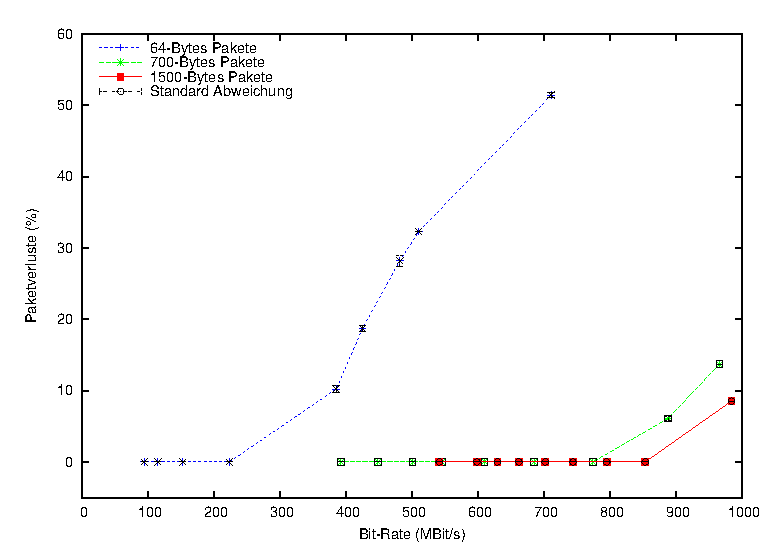
\includegraphics[width=5.5in]{plots/graphs/pktloss_PCI_mbs.eps}
\caption{Paketverluste in Abhängigkeit von der Bit-Rate beim Capturing auf dem Rechner mit dem konventioneller PCI-Bus}
\label{img:plot_pktlos_pci_mbs}
\end{figure}

\begin{figure} 
\centering 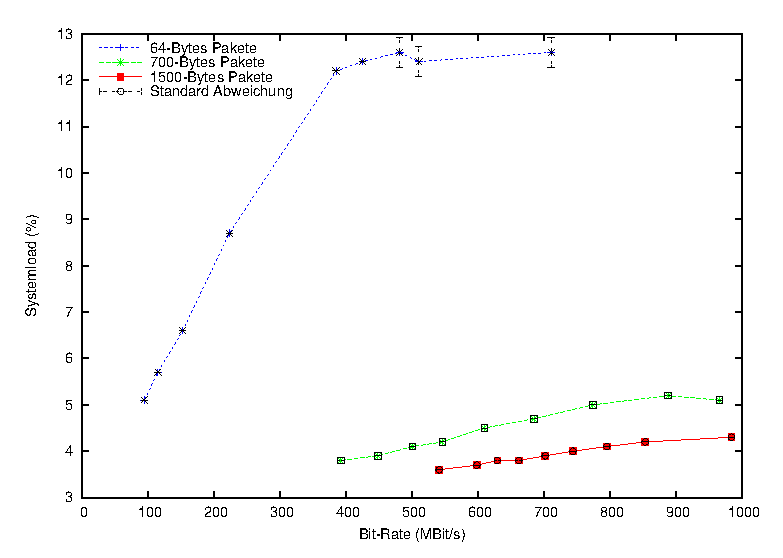
\includegraphics[width=5.5in]{plots/graphs/sysload_PCI_mbs.eps}
\caption{Systemload in Abhängigkeit von Bit-Rate beim Capturing. Konventioneller PCI-Bus}
\label{img:plot_sysload_pci_mbs}
\end{figure}
}
\subsubsection{Vergleich generic- mit ringmap-Paket-Capturing-Stack}\label{sec:erg_verg}
\textbf{Das Ziel} dieses Experiments ist es, die Capturing-Performance von 
\emph{ringmap}-Capturing-Stack mit dem \emph{generic}-Capturing-Stack
zu vergleichen.\\\\
%
Konfiguration auf dem Capturer: 
\begin{itemize}
	\item \textbf{Hardware:} FreeBSD-2 
	\item \textbf{Betriebssystem:} FreeBSD \textbf{7.2}, \textbf{non-SMP Kernel}
	\item \textbf{Treiber:} 
		\begin{itemize}
			\item Paket-Ringpuffer-Größe: 1024 Slots
			\item BPF-Puffer-Größe: 10MB
		\end{itemize}
\end{itemize}
Verkehrsparameter:
\begin{itemize}
	\item Paketlängen: 64-, 200-, 300-Bytes
	\item Paketmengen: 5000000-, 10000000-, 15000000 Pakete 
\end{itemize}

\paragraph*{Paketverluste:}
In Abbildung \ref{img:plot_pktlos_ringmap_vs_generic_mbs} sind die
Paketverluste dargestellt.  Auf der X-Achse wird die generierte Datenrate
dargestellt. Auf der Y-Achse der prozentuelle Anzahl der Paketverluste.  Bei
allen Tests entstanden die Paketverlust bei \emph{generic}-Stack lediglich für
Pakete der Größen 200 und 64 Bytes.  Dabei kann der \emph{generic}-Stack für
die 64-Bytes-Pakete bei der Bit-Rate von 393Mbit/s und höher
(entsprechende Paket-Rate $> 819545$) nur eine konstante Anzahl von Paketen
erfassen, etwa 262147 Pakete, unabhängig von der generierte Paketmenge. 

\paragraph*{Systemload:}
Die Ergebnisse der Systemload-Messung sind in Abbildung
\ref{img:plot_sysload_ringmap_vs_generic} dargestellt. Auf X-Achse wird die
generierte Datenrate dargestellt. Auf der Y-Achse die Systemload.  Bei
Erfassung der Verkehr mit dem \emph{generic}-Stack liegt die Systemload
wesentlich höher als beim \emph{ringmap}-Stack. Dies erklärt sich dadurch, dass
der \emph{generic}-Stack für jedes Paket mehrere Kopie-Operationen im
Kernelspace ausführt und für den Paketzugriff von der Userspace einen
Systemaufruf verwendet. Bei hohen Daten-Raten ist diese Vorgehensweise des
\emph{generic}-Stack nicht mehr effizient.
\begin{figure} 
\centering 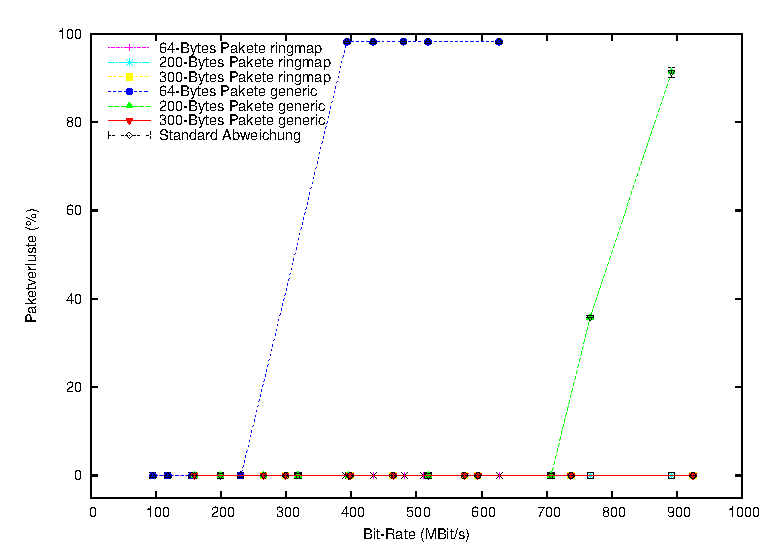
\includegraphics[width=5.5in]{plots/graphs/pktloss_generic_vs_ringmap_mbs.eps}
\caption{Paketverluste in Abhängigkeit von Bit-Rate beim Capturing. Vergleich ringmap- und generic-Packet-Capturing-Stacks}
\label{img:plot_pktlos_ringmap_vs_generic_mbs}
\end{figure}
\begin{figure} 
\centering 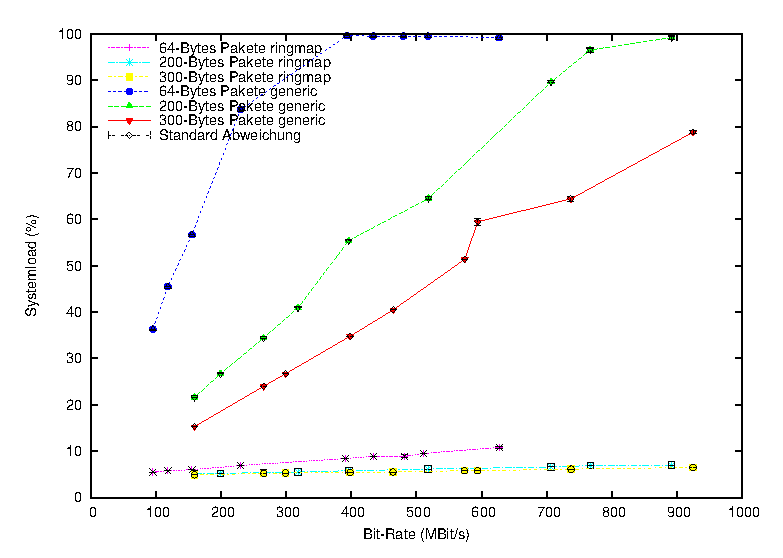
\includegraphics[width=5.5in]{plots/graphs/sysload_generic_vs_ringmap_mbs.eps}
\caption{Systemload in Abhängigkeit von Bit-Rate beim Capturing. Vergleich ringmap- und generic-Packet-Capturing-Stacks}
\label{img:plot_sysload_ringmap_vs_generic}
\end{figure}

\newpage

\section{Zusammenfassung}
Das Ziel dieser Diplomarbeit ist es, die für Capturing relevante Software des
Betriebssystem FreeBSD zu untersuchen, die Probleme, die zur Reduzierung der
Capturing-Performance führen, herauszufinden und aufgrund der gefundenen
Problemen den neuen (ringmap)-FreeBSD-Packet-Capturing-Stack zu erarbeiten,
zu implementieren und auszuwerten. Die neue Lösung basiert auf der für die Diplomarbeit
vorausgesetzte Hardware (siehe Abschnitt \ref{sec:hwsw_voraus}).\\\\
%
Die Diplomarbeit ist in drei Phasen abgelaufen: Einarbeitung, Implementierung
und Testen.  Während der \textbf{Einarbeitungszeit} habe ich viele neue
Kenntnise in Themen, die über das normales Informatiksstudium hinausgehen,
erworben.  Es handelt sich vor allem um Wissen über die Funktionsweise moderner
Netzwerkadapter und Betriebssystemkern- und -Treiber-Programmierung. Unter
Anderem habe ich dabei neue Konzepte über die Hardware-Gegebenheiten und
Software-Implementierung der modernen Interrupt- und DMA-Mechanismen (siehe
Kapitel Grundlagen, Abschnitt \ref{sec:adapter}) gelernt. \\\\
%
Außerdem wurden von mir mehrere Arbeiten~\cite{fabian_da, pcin10gb_paper,
perfev_paper, bpf_paper} über Capturing-Problematik durchgearbeitet mit dem
Ziel, die beim Capturing vorhandene Probleme zu analysieren, um die
Anforderungen für den neuen \emph{ringmap}-Packet-Capturing-Stack zu erstellen.
Für die Capturing-Performance-Probleme wurde in den Arbeiten hauptsachlich die
Anzahl der Paket-Kopie-Operationnen und die hohe Interrupt-Rate bei der
Verkehr-Erfassung als Gründe genannt. Als eine mögliche Lösung zur des
Interrupt-Overhead wird die Verwendung des
\emph{Polling}-Mechanismus~\cite{bsd_polling} vorgeschlagen.  Wegen der
Instabilität der BSD-Polling-Implementierung für
SMP-Kernel~\cite{bsd_devpoll_page} habe ich für den Entwurf des neuen Stacks
allerdings das normale Interrupt-Driven-Modell eingesetzt. Neben der Anzahl der
Kopie-Operationen, wurden im \emph{generic}-Capturing-Stack einige andere
Implementierungsdetails entdeckt, welche die Capturing-Performance bei hohen
Paket-Raten beeinflüssen können. Vor allem die Speicher-Allozierungen welche
der \emph{generic}-Treiber für jedes neue Packet durchführt, beeinflüssen die
Performanz negativ. Mit dem Ziel die herausgefundene
Capturing-Performance-Probleme zu eliminieren wurden die Anforderungen und den
Entwurf der Implementierung des neuen \emph{ringmap}-Packet-Capturing-Stack
erstellt (Kapitel Grundlagen, Abschnitt \ref{sec:aufgstel}).\\\\
%
In der \textbf{Implementierung}-Phase wurde der neue
\emph{ringmap}-Packet-Capturing-Stack für das Betriebssystem FreeBSD
programmiert (siehe Kapitel Implementierung). Dafür wurde der Code für
Adapter-Treiber, Systemaufruf-Funktionen und Libpcap-Library implementiert.
Während der Implementierung  habe ich tiefgehende Kenntnisse und viel
praktische Erfahrung in  Kernel- bzw. Treiberprogramming für
UNIX-artige-Systeme erworben.  \\\\
%
In der \textbf{Test}-Phase wurde der neue \emph{ringmap}-Packet-Capturing-Stack
getestet und mit dem \emph{generic}-Stack in Bezug auf leistungsfähigkeit
vergliechen. Für das Testen des \emph{ringmap}-Stack wurden unterschiedliche
Verkehr-Raten generiert, unterschiedliche Treiber-Parameter eingesetzt und
verschiedene Hardware für den Tets verwendet (siehe Kapitel
Leistungsbewertung). Für die Tests wurden \emph{Shell}-Skripte implementiert
die sowohl alle Testablüfe gesteuert haben als auch die Testergebnisse
ausgewertet und in Form von Tabellen und \emph{gnuplot}-Grafiken gespeichert
haben. 

\subsection{Erreichte Ziele}

\subsubsection{Verbesserung der Capturing-Performance}
Beim Einsatz des im Rahmen der Diplomarbeit implementierten
\emph{ringmap}-Stack wird die Capturing-Performance unter gleichen Bedingungen
höher als beim \emph{generic}-Stack. Die \textbf{Systemload} beim Capturing mit
dem \emph{ringmap}-Stack ist deutlich geringer als mit dem \emph{generic}-Stack.
Bei allen durchgeführten Experimenten war die Systemload beim Capturing mit dem
\emph{ringmap} kleiner als $12\%$. Die Systemload bei der Verwendung von
\emph{generic}-Stack variiert von $13\%$ bis $100\%$. Bezüglich der
Systemload zeigt der \emph{ringmap} einen deutlichen Gewinn.\\\\
%
Anders sieht es mit den \textbf{Paketverlusten} aus. Beide Stacks zeigen
identisch gute ($100\%$) Paketerfassungsrate für den Fall wenn die Paketgröße
über 200 Bytes liegt. Bei Paketen kleiner als 200 Bytes, und daraus
verursachten höheren Paketraten, $> 450000 pkts/sec$, verliert der
\emph{generic}-Stack (mit 10MB BPF-Puffer-Größe) bis zu $100\%$ aller der
generierten Pakete. Selbst bei maximaler Belastung verliert der \emph{ringmap}-Stack 
weniger als $0.02\%$ der Pakete.

\subsubsection{Stabilität und Benutzbarkeit}\label{sec:stab_und_func}
Der \emph{ringmap}-Capturing-Stack hat in der Tests-Phase (insgesamt mehr als
100 000 Tests mit den unterschiedlichen Treiber-Parameter) weder
\emph{Segmentation faults} noch keine \emph{Kernel panics} verursacht. Das
bedeutet, dass die für Kernelspace und Userspace (Libpcap) implementierte
Software sehr stabil ist.\\\\
%
Der \emph{ringmap} ist sehr einfach einzusetzen. Im Verzeichnis 
\verb+scripts/+ befinden sich zwei Shell-Skripts:
\begin{itemize}
	\item \verb+ringmap_build_and_load+: Kompiliert und installiert \emph{ringmap}-Software. 
	\item \verb+generic_build_and_load+: Bringt das System in den generischen Zustand. 
\end{itemize}
Dadurch, dass der Userspace-Code in der Libpcap-Library eingesetzt wurde,
erlaubt es allen Anwendungen, die auf Libpcap basieren, zum Beispiel \emph{tcpdump},
ohne Änderungen  Netzwerk-Pakete mit dem \emph{ringmap}-Stack zu erfassen
(siehe Einschränkungen im nächsten Abschnitt \ref{sec:einschr}).\\\\
%
Zudem lässt sich der \emph{ringmap}-Capturing-Stack, im Fall dass es auf dem 
System mehrere unterschiedliche Intel Gigabit Adapters gibt, durch die 
Eingabe der \emph{PCI-Device-ID} nur für einen ausgewählten Adapter einsetzen, 
sodass der \emph{generic}-\textbf{em}-Treiber die restliche Adapters steuert. 
Die \emph{PCI-Device-ID} des Adapter wird als Makrodefinition \verb+DEV_ID+ in der 
Datei \verb+fiveg_da.h+ eingegeben. Dadurch ist es möglich \emph{ringmap}- und 
\emph{generic}-Software auf einem System gleichzeitig zu benutzen.

\subsection{Einschränkungen des ringmap-Packet-Capturing-Stack}\label{sec:einschr}
Die Benutzung der \emph{ringmap}-Software verursacht auf dem Capturing-System
(bzw. für die Ausgewählte Adapter) folgende Einschränkungen:
\begin{description}
	\item [Kein TCP/IP Protokollstack:] Der \emph{ringmap}-Adapter-Treiber
		besitzt zur Zeit keine Verbindung mit den TCP/IP-Protokoll-Stack-Funktionen.
		Das heißt, dass ein Netzwerk-Interface, das  mit dem
		\emph{ringmap}-Treiber gesteuert wird, zu diesem Zeitpunkt ausschliesslich für
		Paket-Capturing benutzt werden kann. Wenn aber im System mehrere
		Netzwerk-Adapter mit den unterschiedlichen \emph{Device-ID's} vorhanden
		sind, dann ist es möglich den Protokoll-Stack über das andere
		Netzwerkinterface zu benutzen (siehe Abschnitt
		\ref{sec:stab_und_func}).
	\item [Keine Paketfilterung im Userspace:] Die Paket-Filterung mit  BPF
		im Userspace ist derzeit nicht möglich. Das Benutzen von
		BPF-Filter sollte aber keine aufwendige Aufgabe zu sein, denn auch die  Libpcap hat eine 
		Implementierung für BPF. Daher kann Filtern mit den
		Libpcap-Funktionen umgesetzt werden.
	\item [Libpcap Einschränkungen:] Für das Anpassen der Libpcap an den \emph{ringmap}-Stack wurden einige Code-Stücke im
		Libpcap-Quell-Code auskommentiert oder ersetzt. Dadurch ist die
		Funktionalität der neuen \emph{ringmap}-Libpcap ist nicht mit
		der \emph{generic}-Libpcap identisch. Aus der
		\emph{generic}-Libpcap sind die Funktionalität entfernt, welche den
		BPF im Kernelspace anfordern. Außerdem wurde der
		\verb+to_ms+-Parameter~\cite{man_pcap} für die
		\verb+pcap_open_live()+-Funktion deaktiviert, aber aus 
		Kompatibilitätsgründen geblieben. Beim
		Capturing mit dem \emph{ringmap}-Stack blockiert der Userspace-Prozess wenn
		es keine neue Pakete mehr gibt, bis  weitere Pakete ankommen.
\end{description}
Alle genannte Einschränkungen sind  in dem Sinne nicht kritisch, dass 
sie sich eliminieren oder, für bestimmte Anforderungen, anpassen lassen. 
Der Source-Code von \emph{ringmap} ist auf Google-Code veröffentlicht 
und unter dem Namen \emph{ringmap} auf dem Server zu finden. An der  zukünftigen 
Weiterentwicklung des Projektes habe ich großes Interesse und biete meine Hilfe an.

\subsection{Zukünftige Themen}
\subsubsection{Performance-Vergleich mit dem Zero-Copy-BPF-Buffers}
Im Lauf der Test-Phase der Diplomarbeit, war der \emph{Zero-Copy-BPF-Buffers}
Projekt noch im alpha-Stadium und nicht bereit für das Testen (siehe Abschnitt
\ref{sec:verw_bpf}). Inzwischen ist der Zero-Copy-BPF-Buffers in der neusten
FreeBSD-8.0-Version vorhanden und soll stabil sein. Daher soll die Auswertung 
von Zero-Copy-BPF-Buffers der nächste Schritt sein.
\subsubsection{10Gbit Capturing}
Der Source-Code des \textbf{ixgbe}-Adapter-Treibers~\cite{10gbit_adapter_bsd}
für 10-Gigabit-Netzwerkanschlüsse\footnote{\textbf{ixgbe} - Treiber für Intel
10-Gigabit-Netzwerkadapter} hat eine ähnliche Struktur wie der Source-Code des
\textbf{em}-Treiber. Deshalb sollte die \emph{ringmap}-Software einfach für den
10-Gigabit-Treiber anpassbar sein. Dafür muss aber eine Arbeit vom in
FreeBSD-Kernel-Programming kompetenten Spezialisten geleistet werden, denn
beide Treiber sind nicht vollkommen identisch, und deshalb sollte dem
Softwareentwickler alle Details von BSD-Treiber-Programming bekannt werden, um
die Portierung auf 10Gbit zu machen. Auch hierzu biete ich meine Hilfe an.\\\\

\newpage

\newpage
\pagestyle{empty}
\bibliography{main}

\newpage

\lstlistoflistings
\mbox{}
\cleardoublepage
\end{document}
